
% For printing with the A5 format
\documentclass[a4,11pt,twoside,openright,english,italian]{book}% twoside!

% Set paper size
\usepackage[twoside=true]{geometry}

% For printing in a4
\geometry{a4paper,
  margin=3cm,
  top=3.8cm,
  bindingoffset=0.4cm
}

%Uncomment this for final prints: this just enables printing on a4 paper
\usepackage[cam,center,a4,pdflatex,axes]{crop}

\usepackage{phdthesis}

\usepackage{fancyhdr}
\usepackage{color}
\usepackage{array}
\usepackage{mdwmath}
\usepackage{mdwtab}
\usepackage{amsmath,amssymb}
\usepackage{cite}

\usepackage{graphicx}
\graphicspath{{./img/}}

\usepackage{glossaries}
\usepackage{listings}
\usepackage{subfig}
\usepackage{booktabs}
\usepackage{latexsym}
\usepackage{color}
\usepackage{url}
\usepackage{bnf}
\usepackage{rotating}
\usepackage{multirow}
\usepackage{phdtitle}
\usepackage{paralist}
\usepackage{bibentry}
%\usepackage[algochapter]{algorithm2e}
\usepackage[bookmarks=true,pdftex=false,bookmarksopen=true,pdfborder={0,0,0},hidelinks]{hyperref}
\usepackage{lscape}
\usepackage{algorithmic}
\usepackage{algorithm}
\usepackage{longtable}
\usepackage[latin1, utf8x]{inputenc}






\usepackage{indentfirst}

% font sans serif
% \usepackage{arev}
% \usepackage[T1]{fontenc}

% font serif
\usepackage{DejaVuSerif}
\usepackage[T1]{fontenc}


\usepackage{setspace}
\renewcommand{\baselinestretch}{1.5}

\setcounter{tocdepth}{3}
\setcounter{secnumdepth}{3}





%% \hyphenation{} is used to force the 
\hyphenation{}

\newtheorem{Definition}{Definition}[section]

\lstset{tabsize=2,basicstyle=\footnotesize,breaklines=true}

\usepackage[greek,english,italian]{babel}

\usepackage{ulem}
\normalem

\hypersetup{pdftitle={A distributed framework supporting runtime autotuning for HPC applications}, pdfauthor={Cristiano Di Marco}}

\nobibliography*

\department {\normalfont{DIPARTIMENTO DI ELETTRONICA, INFORMAZIONE E BIOINGEGNERIA\\COMPUTER SCIENCE AND ENGINEERING - INGEGNERIA INFORMATICA}} %{Dipartimento di Elettronica, Informatica e Bioingegneria}
\phdprogram{\normalfont{MASTER THESIS}}

\author{Cristiano Di Marco}
\matricola{835911}
\title{A DISTRIBUTED FRAMEWORK\\SUPPORTING RUNTIME AUTOTUNING\\FOR HPC APPLICATIONS} %{A distributed framework supporting runtime autotuning for HPC applications}
\advisor{Cristina Silvano}
\coadOne{Gianluca Palermo}
\coadTwo{Davide Gadioli}
\titleimage{img/logopoli.png}
\phdcycle{Academic year 2016/2017}

%%%%%%%%%%%%%%%%%%%%%%%%%%%%%%%%%%%%%%
% Let's Start The Real Document
%%%%%%%%%%%%%%%%%%%%%%%%%%%%%%%%%%%%%%
\begin{document}
\selectlanguage{english}

\maketitle

\pagestyle{empty}

\cleardoublepage
\newpage

%%%%%%%%%%%%%%%%%%%%%%%%%%%%%%%%%%%%%%
% Dedica
%%%%%%%%%%%%%%%%%%%%%%%%%%%%%%%%%%%%%%
Dedica


\cleardoublepage
\newpage

\pagestyle{fancy}
% change numbering into Roman numbers for the introductory part
\setcounter{page}{1}
\pagenumbering{Roman}

%%%%%%%%%%%%%%%%%%%%%%%%%%%%%%%%%%%%%%
% Abstract and Sommario
%%%%%%%%%%%%%%%%%%%%%%%%%%%%%%%%%%%%%%
\chapter*{Estratto}

\begin{otherlanguage}{italian}

\lettrine{A}{}\textit{pplicazioni} di ricerca avanzata come gli studi sull'universo o sulla microbiologia, stanno proiettando le architetture ad elevate prestazioni di calcolo (\textit{High Performance Computing}) verso il traguardo di un miliardo di miliardi di operazioni effettuate al secondo, atteso nel 2022.

Queste ricerche sono caratterizzate da una enorme quantità di dati in ingresso e dalla presenza di parametri che ne influenzano l'esecuzione. Poichè problematiche inerenti il consumo di potenza e l'efficienza energetica hanno assunto un'importanza rilevante, esistono varie tecniche che tentano di migliorare questi aspetti, mantenendo comunque accettabile il valore dei risultati ottenuti. Strategie di approssimazione (\textit{Ap\-prox\-i\-mate Com\-put\-ing}), applicabili sia a livello hardware sia a livello software, cercano di raggiungere un equilibrio tra la qualità della computazione e lo sforzo richiesto, al fine di adempiere ai vincoli e agli obiettivi dell'applicazione e di massimizzare, al contempo, l'efficienza di calcolo.

Per questo tipo di applicazioni, lo spazio delle possibili configurazioni è molto ampio e, pertanto, non è possibile esplorarlo esaustivamente. Possedere una completa conoscenza riguardo le combinazioni dei parametri e i corrispondenti risultati delle metriche prese in esame (come, ad esempio, il numero di operazioni completate al secondo, il consumo di potenza oppure la precisione dei dati in uscita) è praticamente irrealizzabile e, pertanto, si ricorre a soluzioni approssimate.

Questa tesi ha sviluppato un sistema, \textit{Agorà}, in grado di gestire l'esplorazione di un sottospazio delle possibili configurazioni, con lo scopo di predire, usando tecniche di apprendimento automatico (\textit{Machine Learning}), il modello completo dei programmi in esame; questo risultato è utilizzato da un \textit{autotuner} per sce\-glie\-re dinamicamente la migliore combinazione di parametri che soddisfi vincoli e obiettivi dell'applicazione. I principali benefici apportati da Agorà sono l'eliminazione di ogni fase an\-te\-ce\-den\-te l'esecuzione dei programmi e la capacità di gestire molteplici applicazioni contemporaneamente.

\end{otherlanguage}


\cleardoublepage
\newpage

\chapter*{Abstract}

\lettrine{C}{}\textit{ompute} and data intensive research problems, such as universe or microbiological studies, are pushing High Performance Computing architectures to achieve, in 2022, the Exascale level, that is the capability to process a billion billion calculations per second.

These applications manage huge input datasets and they are characterized by multiple parameters that influence execution. Given that power consumption issues and energy efficiency have become essential, there exist various techniques that try to improve these aspects, keeping on acceptable quality of results. Approximate Computing strategies, both at software and hardware level, balance computation quality and expended effort, in order to achieve application objectives and to maximize overall computational efficiency.

The design space of all possible configurations, for these kind of applications, is very huge and, therefore, it cannot be explored exhaustively. To achieve a full knowledge on both parameter values and corresponding metric of interest (such as throughput, power consumption or output precision) is almost unfeasible and, therefore, we prefer approximate solutions.

This thesis has focused on the development of a framework, \textit{Agora}, that is able to drive online Design Space Exploration through an initial subset of configurations, in order to predict an application complete model through Machine Learning techniques. The result is used by an autotuner to dynamically adapt program execution with the best configuration that fulfills current goals and requirements. Main advantages of Agora are the elimination of any offline phase and design-time knowledge as well as the capability to manage multiple running applications at the same time.


\cleardoublepage
\newpage

%%%%%%%%%%%%%%%%%%%%%%%%%%%%%%%%%%%%%%
% TOC
%%%%%%%%%%%%%%%%%%%%%%%%%%%%%%%%%%%%%%
\renewcommand{\contentsname}{Table of Contents}
\tableofcontents
\cleardoublepage
\newpage

% Now lets go back to normal numbering
\setcounter{page}{1}
\pagenumbering{arabic}

\cleardoublepage
\chapter{Introduction}

\section{Problem and Motivations}

\lettrine{N}{owadays}, increasingly accurate climate forecasts, biomedical researches, business analytics, astrophysics studies or, in general, Big Data related problems require huge computing performance in order to obtain significant results; for these reasons, High Performance Computing technologies have been continuously sped up and, now, their next target is the Exascale level, that is the capability of at least one exaFLOPS, equal to a billion billion FLOPS (FLoating Point Operations Per Second), which is the order of processing power of human brain at neural level, based on H. Markram et al. research study (\cite{markram2011introducing}).

In order to raise computing performances, multicore scaling era has produced, over time, frequency and power increase; it's impossible to follow this trend anymore, due to the beginning of Dark Silicon era (\cite{esmaeilzadeh2011dark}) and the failure of Dennard Scaling (\cite{dennard1974design}): in 1974, Robert H. Dennard provided a more granular view of the famous Moore's Law (\cite{moore1998cramming}) about the doubling of number of transistors, in a dense integrated circuit, approximately every two years; this trend produces faster processors because, as transistors get smaller, their power density is constant, so that power use is proportional with area: as transistors get smaller, so necessarily do voltage and current, giving the possibility to increase frequency. The ability to drop voltage and current, in order to let transistors operate reliably, has broken down; static power (power consumed when transistor is not switching) has increased its contribution in overall power consumption, with an importance similar to dynamic power (power consumed when transistor changes its value), producing serious thermal issues and realistic breakdowns. This scenario implicates the impossibility to power-on all components of a circuit at nominal operating voltage due to Thermal Design Power (TDP) constraints.

Due to these physical problems, system energy efficiency has become essential; even if, every approximately 1.5 years computation per kilowatt-hour have doubled over time (\cite{koomey2011implications}), Subramaniam et al. investigation (\cite{subramaniam2013trends}) suggests that there is the need of an energy efficiency improvement at a higher rate than current trends, in order to reach target consumed power of 20 MW for Exascale systems, established by DARPA report (\cite{bergman2008exascale}).

Efficiency has become very important also for electricity consumption of data centers: in fact, just the US data centers are expected to consume 140 billion kWh in 2020, from 61 billion kWh in 2006 and 91 billion kWh in 2013 (\cite{site:NRDC2015}), since the amount of information managed by worldwide data centers is going to grow 50-fold while the number of total servers is going to increase only 10-fold (\cite{gantz2011extracting}).

It is straightforward, therefore, that green and heterogeneous approaches have to be applied in order to improve general efficiency of High Performance Computing architectures in which, for instance, multiple Central Processing Units (CPUs), General-Purpose computing on Graphics Processing Units (GPGPUs) and Many Integrated Cores accelerators (MICs) coexist and work together in a parallel way; for these reasons, \textit{TOP500 Green Supercomputers} (\cite{site:topGreen500}) demonstrates the large interest in green architectures, ranking and updating world top 500 supercomputers by energy efficiency.

There exist various approaches in order to deal with these problems, from both hardware and software point of view; for instance, Power Consumption Management consists of various techniques such as Dynamic Voltage and Frequency Scaling (DVFS) and Ther\-mal-aware or Ther\-mal-management technologies in order to deal with Dark Silicon issue (\cite{mittal2014power}); another important concept is Approximate Computing (\cite{mittal2016survey}), that focuses on balancing computation quality and expended effort, both at programming level and in different processing units; this thesis deals with this last technique, exploited at software level, oriented to tunable High Performance Computing applications that follow the so called \textit{Autonomic Computing} research project (\cite{kephart2003vision}). The underlying structure on which this theory is based is the Monitor-Analyze-Plan-Execute feedback loop: these systems have the capability to manage themselves, given high-level objectives and application knowledge in terms of possible configurations, made by parameter values (such as, for instance, number of threads or processes involved, possible various kind of compiler optimization levels, application-specific variable values, etc.) and the corresponding metric of interest values (such as, for instance, power consumption, throughput, output error with respect to a target value, etc.); this information assembles application Design Space.

Since, for these kind of programs, the multitude of parameters and their corresponding set of values make Design Space huge and since, in general, computation time is not negligible, an exhaustive search is practically unfeasible, so there exist Design Space Exploration techniques that aim to provide approximated Pareto points, namely those configurations that solve better than others a typical multi-objective optimization problem (for instance, keeping throughput above some value while limiting output error and power consumption within a prearranged interval).

Typically, application knowledge is built at design-time; after that, it is passed to a dynamic autotuner that has the ability to choose, from time to time, the best possible set of parameter values (also called \textit{dynamic knobs}) with respect to current goals and requirements that might change during execution.

One of the leading researches in this area is the ANTAREX project (\cite{silvano2016antarex}) that aspires to express by LARA (\cite{cardoso2012lara, cardoso2014performance}), a Domain Specific Language (DSL), application self-adaptivity and to autotune, at runtime, applications oriented to green and heterogeneous HPC systems, up to the Exascale level.





\section{Objectives}

Main objective of this work is to fulfill application Design Space Exploration at runtime, collecting all information about used parameter values and related performances in terms of associated metrics of interest; through this data and Machine Learning techniques, we aim to predict application complete model, made by the whole possible configuration list; finally, obtained model is used by the dynamic online autotuner, that can finally set up related program execution in the best way, according to current goals and requirements.

Agorà feature is the ability to wisely manage multiple tunable applications that run inside a parallel architecture; we want not only to simultaneously supervise different programs, but also to share Design Space Exploration phase among all nodes that run the same application, hence speeding up this process.

Any kind of prior offline phase and design-time knowledge, that separates applications from their execution in runtime autotuning mode, is therefore avoided; Agorà makes autotuning completely independent from both application type and technical specifications about the machine in which program is executed: Agorà does not have to know this information before it starts and final complete model is suitable regardless autotuner objectives.





\section{Thesis structure}

This thesis is structured as follow: in chapter \ref{back} we focuse on the background of concepts connected to our work, clarifying what is a parallel architecture, the meaning of \textit{Design Space Exploration} and \textit{Design of Experiments}, the concept of \textit{dynamic autotuning} and, finally, we present the MQTT messaging protocol and the Generalized Linear Regression (GLR) approach for application model prediction, used in our framework; chapter \ref{sota} gives an overview of the State-of-the-art about principal methodologies related to \textit{Agorà}, in particular on Design Space Exploration and autotuning current research studies; in chapter \ref{methodology} we address our intent, describing overall context, our suggested proposal, its general description and main strenghts; chapter \ref{agora} shows technical implementation of \textit{Agorà} use cases, related workflow and framework behavior; in chapter \ref{exps} we collect all experimental results we have done, in order to validate our project and to highlight overall produced benefits; finally, chapter \ref{end} summarizes entire work, obtained results and possible future \textit{Agorà} developments.
 % uncomment if you want part I
\chapter{Background}\label{back}

\lettrine{I}{}\textit{n} this Chapter, we explain the main concepts and used tools related to Agora. This work has been thought for HPC applications that run in parallel architectures, so we start clarifying what are these target systems and how they are built. After that, we explain the concepts of Design Space Exploration and Design of Experiments, that represents the kernel of this work, together with the idea of application dynamic online autotuning. Finally, we present the tools used for communications among Agora components and for application complete model prediction, highlighting their principal characteristics and features: the Message Queue Telemetry Transport (MQTT) messaging protocol and the Generalized Linear Regression interface by Apache Spark\textsuperscript{TM} Machine Learning MLlib library.

\section{Target architecture}

High Performance Computing applications have complex and massive tasks to do, so they need huge computing power in order to accomplish their objectives.

Parallel computing (\cite{barney2012introduction}) simultaneously uses multiple re\-sourc\-es in order to solve a computational problem, taking advantage of concurrency, that is the possibility to execute, at the same time, those parts that are independent each other. In figure \ref{fig::pC::serial} we can see an example of serial computation, with a single processor that executes problem instructions sequentially, one after another. Figure \ref{fig::pC::parallel} instead represents a possible parallel computation, where problem is split in four parts that can be executed concurrently on different processors.

\begin{figure}[htb]

    \centering

    \subfloat[][\emph{Serial computation}\label{fig::pC::serial}]
        {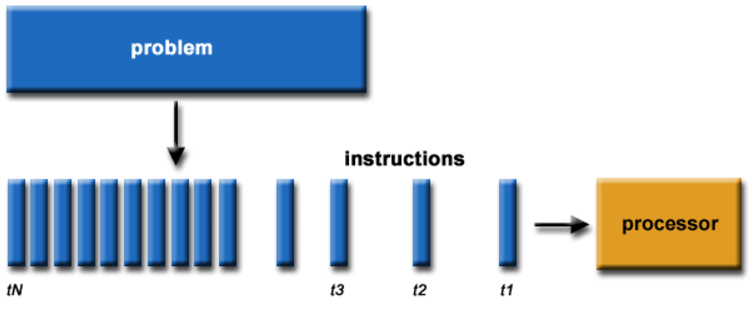
\includegraphics[width = 0.49\textwidth]{ser_prob}}
    \enskip
    \subfloat[][\emph{Parallel computation}\label{fig::pC::parallel}]
        {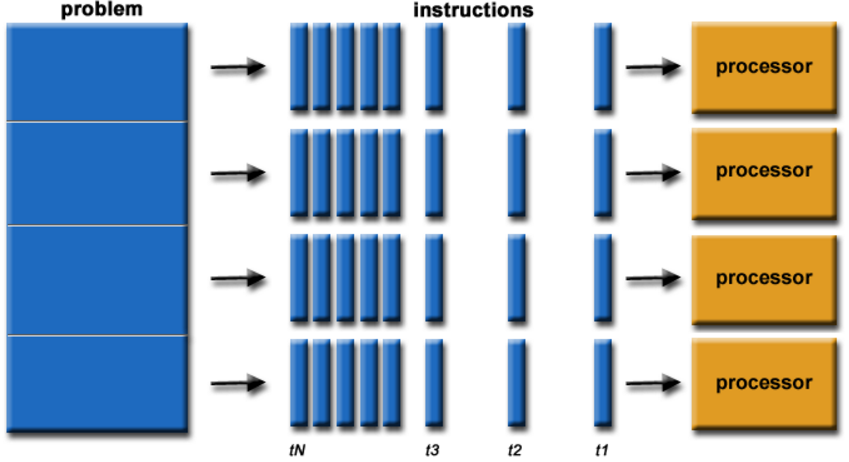
\includegraphics[width = 0.49\textwidth]{par_prob}}
    
    \caption{Serial and parallel computation of a problem}

\end{figure}

A typical parallel architecture is composed by an arbitrary number of computers, called \textit{nodes}, each of them with multiple processors, cores, functional units, ect. connected all together by a network.

\begin{figure}[htb]

    \centering
    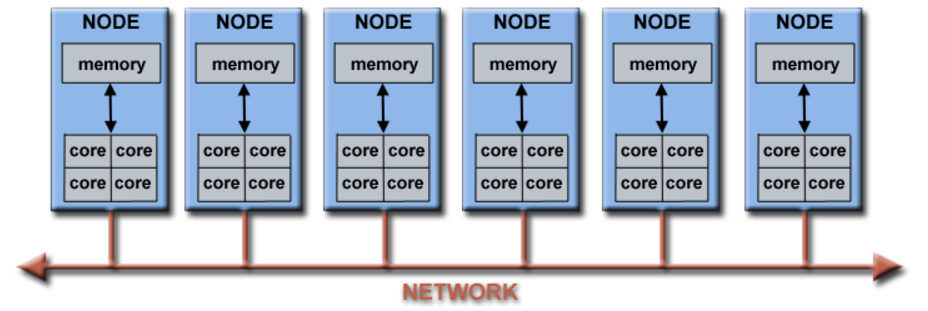
\includegraphics[width = \textwidth]{par_net}
    \caption{Parallel architecture schema}

\end{figure}

Inside a parallel architecture there can be heterogeneous nodes, with different computing techniques and configurations; according to Flynn's classical taxonomy, we can identify four different ways to classify computing architectures: 

\begin{enumerate}

    \item \textit{Single Instruction, Single Data (SISD)}: this is the original kind of computer, in which there is only one instruction stream that is managed by the Central Processing Unit (CPU) during clock cycles. This is serial, so non-parallel, computing;
    
    \item \textit{Single Instruction, Multiple Data (SIMD)}: at any clock cycle, there is one instruction that is executed, but processing units can operate on different data elements of instruction;
    
    \item \textit{Multiple Instruction, Single Data (MISD)}: a single data stream is managed by multiple processing units, that can independently operate on data through separate instruction streams;
    
    \item \textit{Multiple Instruction, Multiple Data (MIMD)}: every processing unit can execute different data and instruction streams.

\end{enumerate}

Nowadays, among introduced alternatives, MIMD architectures are the most used in parallel computing, especially in HPC systems.





\section{Design Space Exploration}

In many engineering problems there are several objectives that have to be obtained, given certain constraints and with the possibility to manage some customizable parameters. Objectives can involve various metrics of interest, for instance connected to application throughput, system consumed power or overall cost.

Automatic Design Space Exploration (DSE) analyzes, in a systematic way, the space of possible parameter combinations that constitute application Design Space, with the objective to find the best design point that fulfills problem goals and requirements.

HPC applications have almost always a lot of parameters and related set of values, making the list of program configurations very long. In these cases, the corresponding Design Space literally explodes, making impossible to analyze it in an exhaustive way.

\subsection{Multi-Objective Optimization (MOO) problem}

When there is more than one objective function, DSE consists of a Multi-Objective Optimization (MOO) problem. Taking \cite{caramia2008multi} as reference, in mathematical terms a MOO problem can be defined as:

\begin{equation}
        min( f_1(x), f_2(x), ..., f_k(x) ), \quad k \ge 2 \qquad s.t. \quad x \in X
\end{equation}

where $k$ denotes the number of objective functions and $X$ represents the feasible region, defined by some constraints functions (for instance, in an embedded architecture, the total area should not exceed a predetermined value). If some of the objective functions have to be maximized, they can be attributed to minimizing its negation.

Multi-Objective Optimization problem has a lot of analogies into a wide variety of situations and domains, even the most common ones. Formerly the ancients, given a set of seeds and a plot of land, had to choose what, how and how much farm, in order to maximize harvest profit and to minimize required effort, simultaneously not exceeding a cost limit. Airline companies want to augment the number of passengers on their airplanes, to increase safety, to enlarge autonomy of their vehicles by means of various technical, strategic and commercial choices. An undergraduate student would minimize his/her university career duration and maximize his/her exam average, with a predetermined time limit and with the possibility to choose some coursers than others.

Since some objectives are in contrast with other objectives, a unique solution does not exist. For instance, in a microcontroller, an objective focused on performance would definitely confront against a goal related to power consumption: best solution for one of them would be the worst for the other and conversely. Therefore, the aim of Design Space Exploration is almost always to search for a trade off, among goals and requirements, that fulfills overall problem.

Since the concept of unique optimal solution can't be applied, it is useful to introduce the notion of Pareto optimality. Pareto optimal solutions are, essentially, those ones that can't be improved without degrading at least one objective function. So, a solution \textit{x\textsuperscript{1}} is said to \textit{(Pareto) dominate} a solution \textit{x\textsuperscript{2}} if:

\begin{equation}
\begin{cases}
        f_i(x^1) \le f_i(x^2) \quad \forall i \in \{1, 2, ..., k\} \\
        f_j(x^1) < f_j(x^2) \quad \textit{for at least one } j \in \{1, 2, ..., k\}
\end{cases}
\end{equation}

The set of Pareto optimal solutions is often called Pareto front, Pareto frontier or Pareto boundary.





\section{Design of Experiments}\label{doe}

When a Design Space of an application is huge and, consequently, there is no possibility to do an exhaustive analysis of all possible configurations, there is the need to take a subset of points of interest that represent as closely as possible system behavior. Therefore, on one hand there is the quality of representation, that should be reliable enough; on the other side, the number of simulations to do, that should be small.

Taking \cite{natrella2013nist} as reference, among various DoE techniques that generate initial set of design points to be analyzed, we can mention:

\begin{itemize}

    \item \textit{Full-Factorial DoE}: it is given by all possible combinations among parameter values, so all possible application configurations are picked up;
 
    \item \textit{2-Level Full-Factorial DoE}: suitable for designs with two or more parameters, this DoE picks up all possible combinations among the extreme values of all parameters.
    
    If, for instance, there are three tunable parameters:
    
    \begin{enumerate}
    
        \item Number of Processors $\in$ \{ 2, 4, 8, 16, 32 \};
        
        \item Number of Threads $\in$ \{ 1, 2, 3, 4, 5, 6, 7, 8 \};
        
        \item Cache size $\in$ \{ 2K, 4K, 8K, 16K, 32K \}.
    
    \end{enumerate}
    
    design points will be: \hbox{$\langle$ \#processors, \#threads, cache size $\rangle$} $\in$
    
    \{ $\langle$ 2, 1, 2K $\rangle$, $\langle$ 32, 1, 2K $\rangle$, $\langle$ 2, 8, 2K $\rangle$, $\langle$ 32, 8, 2K $\rangle$, \hbox{$\langle$ 2, 1, 32K $\rangle$}, \hbox{$\langle$ 32, 1, 32K $\rangle$}, $\langle$ 2, 8, 32K $\rangle$, $\langle$ 32, 8, 32K $\rangle$ \};

    \item \textit{Face Centered Central Composite DoE with one Center Point}: also this DoE is appropriate for designs with two or more parameters. Design point list can be split in three sets:
    
     \begin{enumerate}
    
        \item A 2-Level Full-Factorial Design set;
        
        \item A Center Point, in which each value is the median value of corresponding parameter;
        
        \item An Axial Point set, in which all median and extreme values of each parameter are combined.
    
    \end{enumerate}
    
    Considering the example in previous DoE, final design point list would be: $\langle$ \#processors, \#threads, cache size $\rangle$ $\in$
    
    \{ $\langle$ 2, 1, 2K $\rangle$, $\langle$ 32, 1, 2K $\rangle$, $\langle$ 2, 8, 2K $\rangle$, $\langle$ 32, 8, 2K $\rangle$, \hbox{$\langle$ 2, 1, 32K $\rangle$}, \hbox{$\langle$ 32, 1, 32K $\rangle$}, $\langle$ 2, 8, 32K $\rangle$, $\langle$ 32, 8, 32K $\rangle$ \} $\cup$ 
    
    \{ $\langle$ 8, 4, 8K $\rangle$ \} $\cup$
    
    \{ $\langle$ 2, 4, 8K $\rangle$, $\langle$ 32, 4, 8K $\rangle$, $\langle$ 8, 1, 8K $\rangle$, $\langle$ 8, 8, 8K $\rangle$, $\langle$ 8, 4, 2K $\rangle$, \hbox{$\langle$ 8, 4, 32K $\rangle$} \};
    
    \item \textit{Plackett-Burman DoE}: it might be useful to analyze, more eonomically, a larger number of parameters. This DoE reduces the number of potential factors, constructing very economical designs with number of points multiple of 4 (rather than power of 2, as in the 2-Level Full-Factorial DoE).
    
    Concerning the example above, in this case final design point list would be: $\langle$ \#processors, \#threads, cache size $\rangle$ $\in$
    
    \{ $\langle$ 2, 1, 32K $\rangle$, $\langle$ 32, 1, 2K $\rangle$, $\langle$ 2, 8, 2K $\rangle$, $\langle$ 32, 8, 32K $\rangle$ \};
    
    \item \textit{Latin-Hypercube DoE}: this DoE randomly chooses parameter values for each design point. The number of final configurations can be set up in advance.

\end{itemize}





\section{Dynamic Autotuning}

When applications expose some configurable parameters (a.k.a. \textit{dynamic knobs}), the concept of Dynamic Autotuning is defined as the capability to find the best set of knob values, in an automatic and systematic way, that satisfies application goals and requirements at runtime, properly reacting to possible objective function change. For instance, a web video streaming application would be able to manage video quality according to the overload of its servers. In some situations, it could set up itself for the best possible resolution. Sometimes, it should reduce the quality in order to make still available its services to all connected clients.

IBM research studies on \textit{Autonomic Computing} (\cite{kephart2003vision}, \cite{computing2006architectural}) made a breakthrough on the concept of self-adapting systems that are able to manage themselves and to dynamically optimize their execution configuration at runtime. \textit{Autonomic Computing} is based of the MAPE-K control loop, showed in Figure \ref{fig::mape-k}.

\begin{figure}[htb]

    \centering
    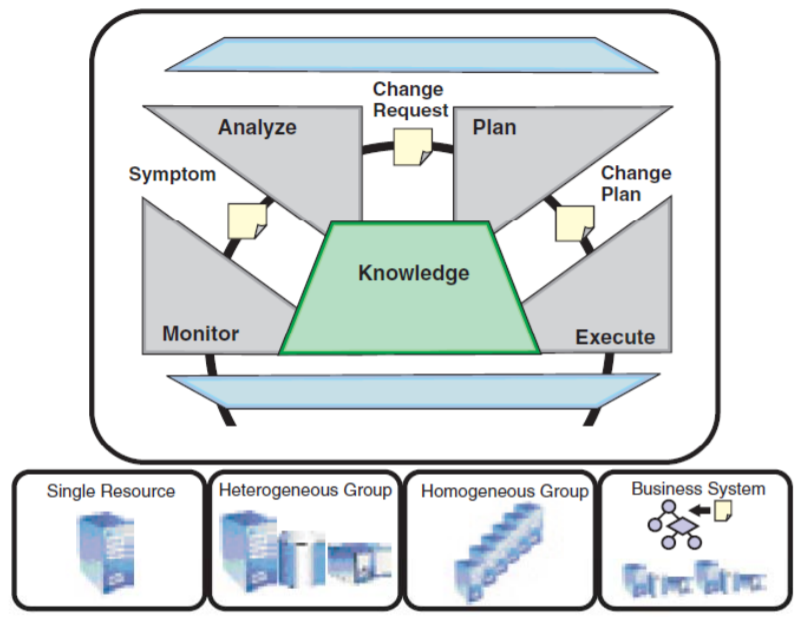
\includegraphics[width = \textwidth]{MAPE-K}
    \caption{MAPE-K control loop design}
    \label{fig::mape-k}

\end{figure}

In this control loop we can identify four principal functions:

\begin{itemize}

    \item \textit{Monitor}: it gathers application information about knob setting and associated metric of interest values as, for instance, throughput and consumed power;
    
    \item \textit{Analyze}: it performs data analysis and reasoning on information provided by the monitor function;
    
    \item \textit{Plan}: it reacts to a possible application objective change during execution and it structures the actions needed to achieve this new state;
    
    \item \textit{Execute}: it modifies the behavior of managed resource, according to actions recommended by the plan function.

\end{itemize}

Finally, \textit{Knowledge} source is composed of all data that is used by the four functions; it includes information such as, for instance, topology structure, historical logs, metrics and policies.

Online autotuning, therefore, entrusts system management from people to technology, achieving self-configuration and self-op\-ti\-mi\-za\-tion objectives. Application requirements may change during execution and the overall system is able to properly react and to re-adapt itself.





\section{MQTT messaging protocol}\label{mqtt}

MQTT (Message Queue Telemetry Transport, \cite{banks2014mqtt}) is a light\-weight messaging protocol that gives the possibility to establish remote communications among subjects. Its main characteristics are the minimization of network bandwidth and devices requirements. This features make MQTT ideal for machine-to-machine (M2M) or Internet of Things (IoT) world of connected devices, but in general this protocol have a large use in different projects; for instance, famous Facebook Messenger is built on top of it (\cite{zhang2011building}).

MQTT uses a client server publish\slash{}subscribe pattern. A client has the possibility to subscribe to topics and to publish messages on them (both topics and messages are strings). Another component, called \textit{broker} server, deals with the dispatch of messages to only clients that have subscribed to corresponding topic. Therefore, publishers (clients that sends messages) and subscribers (clients that receive messages) don't know about the existence of one another: the broker, which is known by every client, distribute messages accordingly. Figure \ref{fig::mqtt_example} shows a possible MQTT scenario with a sensor and two devices.

\begin{figure}[htb]

    \centering
    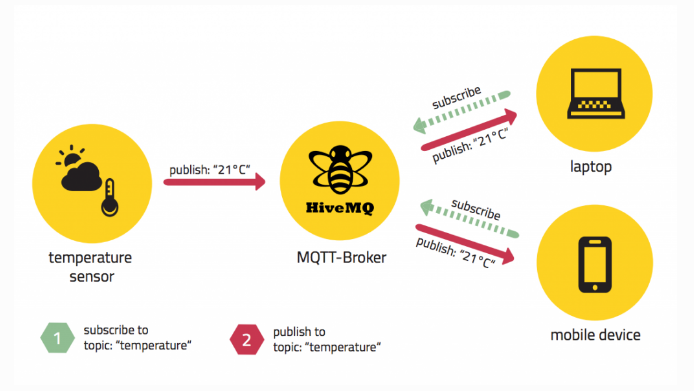
\includegraphics[width = \textwidth]{mqtt}
    \caption{MQTT publish/subscribe example, taken from \cite{site:hivemq}}
    \label{fig::mqtt_example}

\end{figure}

Topics are used by the broker to filter messages and to manage them in a correct way; they are made up of one or more levels, separated by a forward slash, as shown in Figure \ref{fig::topic}.

\begin{figure}[hb]

    \centering
    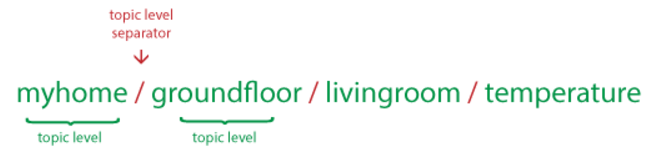
\includegraphics[width = \textwidth]{mqtt_toplevs}
    \caption{A MQTT topic, taken from \cite{site:hivemq}}
    \label{fig::topic}

\end{figure}

There is the possibility to subscribe to more topics at once through the use of wildcards: the single-level one (denoted with the symbol \textit{+}) and the multi-level one (indicated with the symbol \textit{\#}).

Single-level wildcard substitutes an arbitrary level in a topic, so all topics that matches the same structure are associated to the one with single-level wildcard.
For instance,\\
\centerline{\textit{myhome\slash{}groundfloor\slash{}kitchen\slash{}temperature}}\\
\centerline{and}\\
\centerline{\textit{myhome\slash{}groundfloor\slash{}livingroom\slash{}temperature}}\\
match topic in Figure \ref{fig:mqtt_singlew}, while\\
\centerline{\textit{myhome\slash{}groundfloor\slash{}kitchen\slash{}humidity}}\\
don't.

\begin{figure}[htb]

    \centering
    
\includegraphics[width = 0.8\textwidth]{mqtt_singlew}
    \caption{A MQTT topic with single-level wildcard, taken from \cite{site:hivemq}}
    \label{fig:mqtt_singlew}

\end{figure}

Multi-level wildcard is placed at the end of a topic and it covers an arbitrary number of topic levels.
In this case, for instance,\\
\centerline{\textit{myhome\slash{}groundfloor\slash{}kitchen\slash{}tem\-per\-a\-ture}}\\
\centerline{and}\\
\centerline{\textit{myhome\slash{}groundfloor\slash{}kitchen\slash{}humidity}}\\
match topic in Figure \ref{fig:mqtt_mulw}, while\\
\centerline{\textit{myhome\slash{}firstfloor\slash{}livingroom\slash{}temperature}}\\
don't.

\begin{figure}[htb]

    \centering
    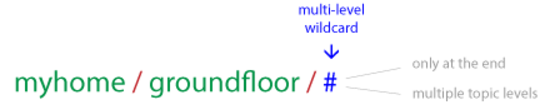
\includegraphics[width = 0.8\textwidth]{mqtt_mulw}
    \caption{A MQTT topic with multi-level wildcard, taken from \cite{site:hivemq}}
    \label{fig:mqtt_mulw}

\end{figure}

Another interesting MQTT feature is the Last Will and Testament (LWT). Each client can specify a normal MQTT message with topic and payload. When it connects to the broker, this message is stored; if client abruptly disconnects, broker sends corresponding LWT to all subscribed clients on related topic, notifying occurred disconnection.





\section{Apache Spark\texorpdfstring{$^{TM}\;$}MMLlib library}

Agora takes advantage of the Machine Learning MLlib library by Apache Spark\textsuperscript{TM} (\cite{spark2015apache}) in order to predict complete model of running applications; in particular, we focuse on the Generalized Linear Regression interface.


\subsection{(Generalized) Linear Regression}\label{glr}

Taking \cite{site:caltechML2012} as reference, Linear Regression tries to model the relationship between a variable $y$ and one or more variables $x_1,x_2,...x_n,n\ge1$. More rigorously, given a set of statistical units $\{y_i,x_{i1},x_{i2},...,x_{ip}\}_{i = 1}^n$, in which $y_i$ is the variable that depends on the p-vector $[x_{i1}, x_{i2}, ..., x_{ip}]$, linear regression assumes that this relationship is linear:

\begin{equation}
    y_i = \beta_0\boldsymbol{1} + \beta_1x_{i1} + \beta_2x_{i2} + ... +  \beta_px_{ip} + \epsilon_i, \quad i = 1, 2, ... n
\end{equation}

$y_i$ is the \textit{response variable} or \textit{regressand};

$x_{i1}, x_{i2}, ..., x_{ip}$ are called \textit{independent variables} or \textit{regressors};

$\beta_0, \beta_1, ..., \beta_p$ are the \textit{regression coefficients}, whose values establish the relationship among regressand and regressors; $\beta_0$ is also called \textit{intercept}. Linear regression mainly focuses on the estimation of these parameters;

$\epsilon_i$ is called the \textit{error term}. It represents all other factors that influence $y_i$ other than the independent variables.

Linear Regression assumes that the response variable follows a Gaussian distribution. Generalized Linear Regression (GLR) gives the possibility to specify other distributions taken from the exponential family. It is useful for several kinds of prediction problems, including Linear Regression, Poisson Regression (for count data) and Logistic Regression (for binary data). Moreover, GLR gives the possibility to specify the link function \textit{g} that relates the mean of regressand to the independent variables. In case of Gaussian distribution for Linear Regression, the link function can be equal to \textit{Identity}, \textit{Log} and \textit{Inverse}, with explicit meaning.


\subsection{Regressor transformations}\label{regrTransforms}

In order to use Linear Regression even if the relationship among response variable and independent variables is not linear, there is the necessity to modify input variables. Agora implements two possible independent variable transformations:

\begin{enumerate}

    \item it transforms parameter values with inverse, square root and natural logarithmic functions. In union with the unaltered predictor variables, it tries to find the best model combining these transformations and available link functions. We refer to this strategy as \textit{"transformations by functions"};
    
    \item it transforms parameter values through polynomial combinations of degree 2: their cross-products and square values are added to the set of regressors, evaluating the best model with available link functions. We refer to this strategy as \textit{"polynomial combinations of degree 2"}.

\end{enumerate}

Agora chooses the model with the smallest Akaike Information Criterion (AIC) value, that is a measure of the quality, in terms of lost information, of statistical models for a given set of data. At the same AIC value, chosen model is the one with the smallest mean of the sum of coefficient standard errors, that measure how precisely predicted model has estimated regression coefficients with the given training set of data.

\chapter{State of The Art}\label{sota}

\lettrine{W}{e} introduce all those works that have been a starting point for the design and implementation of tesiCris; we divide them in two subcategories: the former is oriented to Design Space Exploration, the latter on autotuning.

\section{Design Space Exploration related works}

ReSPIR (\cite{palermo2009respir}) proposes a DSE methodology for application-specific multiprocessor systems-on-chip (MPSoCs). First, a Design of Experiments phase is used to capture an initial plan of experiments that represent the entire target Design Space to be explored by simulations; after that, Response Surface Methodology techniques (\cite{khuri2010response}) identify the feasible solution area with respect to the system-level constraints, in order to refine the Pareto configurations until a predetermined criterion is satisfied.

MULTICUBE Explorer (\cite{silvano2011multicube}) is an open source, portable, automatic Multi-Objective Design Space Exploration framework for tuning multi-core architectures; a designer, through an existing executable model (use case simulator) and a Design Space definition XML file, can easily explore his parametric architecture.

$\epsilon$-Pareto Active Learning ($\epsilon$-PAL, \cite{zuluaga2016e}) aims at efficiently localize an $\epsilon$-accurate Pareto frontier in Multi-Objective Optimization problems; it models objectives as Gaussian process models, in order to guide the iterative design evaluation and, therefore, to maximize progress on those configurations that are likely to be Pareto optimal.

ReSPIR and MULTICUBE are researches oriented on application-specific architectures design, while $\epsilon$-PAL deals with the MOO problem in a general way; all these three works aims to obtain a Pareto front and their execution is done offline; tesiCris uses the concept of Design Space Exploration but it is focused on Approximate Computing software strategies in executing applications; tesiCris doesn't calculate Pareto frontier, but its goal is to provide complete applications model through Machine Learning techniques; moreover, with respect to ReSPIR, MULTICUBE and $\epsilon$-PAL, we want to avoid any offline DSE phase, driving it during programs execution.

Furthermore, at the best of our knowledge, tesiCris is the first framework that is able to fulfill application Design Space Exploration in a shared way, among simultaneously running applications; with this improvement, DSE executing time is considerably reduced. 

\section{Autotuning related works}

SiblingRivalry (\cite{ansel2012siblingrivalry}) proposes an always online autotuning framework that uses evolutionary tuning techniques (\cite{coello2007evolutionary}) in order to adapt parallel programs. It eliminates the offline learning step: it divides available processor resources in half and it selects two configurations, a "safe" one and an "experimental" one, according to an internal fitness function value; after that, the online learner handles the identical current request in parallel on each half and, according to the candidate that finishes first and meets target goals and requirements, it updates its internal knowledge about configurations just used. This technique is used until a convergence is reached or when the context changes and, therefore, new objectives have to be achieved. When objectives change, SiblingRivalry restarts its procedure until new result is obtained; tesiCris doesn't ground its worklow on predetermined objectives: it is completely uninteresting about application goals and requirements, since it predicts the complete model for all metrics under examination; furthermore, computational power of the machine in which the tunable program is executed is not kept busy by tesiCris, since application information gathering and model prediction are done remotely, on a different computer.

Capri framework (\cite{sui2016proactive}) focuses on control problem for tunable applications which mostly use Approximate Computing (\cite{mittal2016survey}) as improvement technique; given an acceptable output error, it tries to minimize computational costs, such as running time or energy consumption. There are two main phases: training, done offline, estimates error function and cost function, using machine learning techniques with a training set of inputs; the control algorithm, done online, finds the best knobs setting that fulfills objectives. Also tesiCris is oriented in tuning applications based on Approximate Computing techniques; it is focused on everything that precedes the control phase, supplying, to the dynamic online autotuner, metrics of interest estimations for each possible application configuration; tesiCris wants to eliminate any offline phase, giving the possibility to simply run an application, driving its execution in order to collect a training set for model prediction; finally, the result is transmitted to application autotuner, that is in charge of managing the control phase.

mARGOt (\cite{gadioli2015application}) proposes a lightweight approach to application runtime autotuning for multicore architectures; it is based on the Monitor-Analyze-Plan-Execute (MAPE) feedback loop (\cite{kephart2003vision}), made up of a complex and varied monitors infrastructure and an Application-Specific RunTime Manager (AS-RTM), based on Barbeque work (\cite{bellasi2012rtrm}): the first captures runtime information that is used by the latter in order to tune application knobs, together with design-time knowledge and application multi-objective requirements. The user has to provide XML configuration files in which a list of mARGOt Operating Points, desired monitors and application objectives are expressed; the AS-RTM module, starting from this design-time knowledge and evaluating runtime information, has the task of choosing, from time to time, the best application configuration that satisfies application goals and requirements as best as possible. This work has been the starting point for the conception of tesiCris framework; mARGOt has to have the list of program configurations before execution: we want to produce this information while applications are running, removing to users the burden to make an offline step before taking advantage of autotuner capabilities.

There are other different autotuning frameworks in HPC context, yet based on design-time knowledge: OpenTuner (\cite{ansel2014opentuner}) is able to build up domain-specific program autotuners in which users can specify multiple objectives; ATune-IL (\cite{schaefer2009atune}) is an offline autotuner that gives the possibility to specify a wide range of tunable parameters for a general-purpose parallel program; PetaBricks (\cite{ansel2009petabricks}) is oriented on the definition of multiple algorithms implementations to solve a problem; \cite{tiwari2009scalable} proposes a scalable and general-purpose framework for autotuning compiler-generated code, combining Active Harmony's parallel search backend (\cite{chung2004using}) and the CHiLL compiler transformation framework (\cite{chen2008chill}); Green (\cite{baek2010green}) is focused on the energy-conscious programming using controlled approximation; PowerDial (\cite{hoffmann2011dynamic}) is a system that transforms static configuration parameters into dynamic knobs in order to adapt applications behavior with respect to the accuracy of computation and the amount of resources. tesiCris main difference is the absence of any kind of prior information about application features and the indifference on quality and quantity of metrics and objectives, in contrast with the last two mentioned works (\cite{baek2010green} and \cite{hoffmann2011dynamic}), focused on energy and accuracy goals.

Finally, among libraries for specific tasks, OSKI (\cite{vuduc2005oski}) provides a collection of low-level primitives that automatically tunes computational kernels on sparse matrices; SPIRAL (\cite{puschel2004spiral}) generates fast software implementations of linear signal processing transforms; ATLAS (\cite{whaley1998automatically}) builds up a methodology for the automatic generation of highly efficient basic linear algebra operations, focusing on matrix multiplications. tesiCris aims to generalize autotuning process.

\chapter{Proposed Methodology}\label{methodology}

\lettrine{T}{}\textit{unable} applications are characterized by the presence of specific parameters, also known as \textit{knobs}, that influence program execution; their change generates different application results in terms of metric of interest values, as, for instance, throughput or power consumption. Figure \ref{fig::appDef} shows a typical parallel architecture with three nodes (node 1, 2 and 3) that are executing three tunable applications (application X, Y and Z respectively):

\begin{figure}[H]

    \centering
    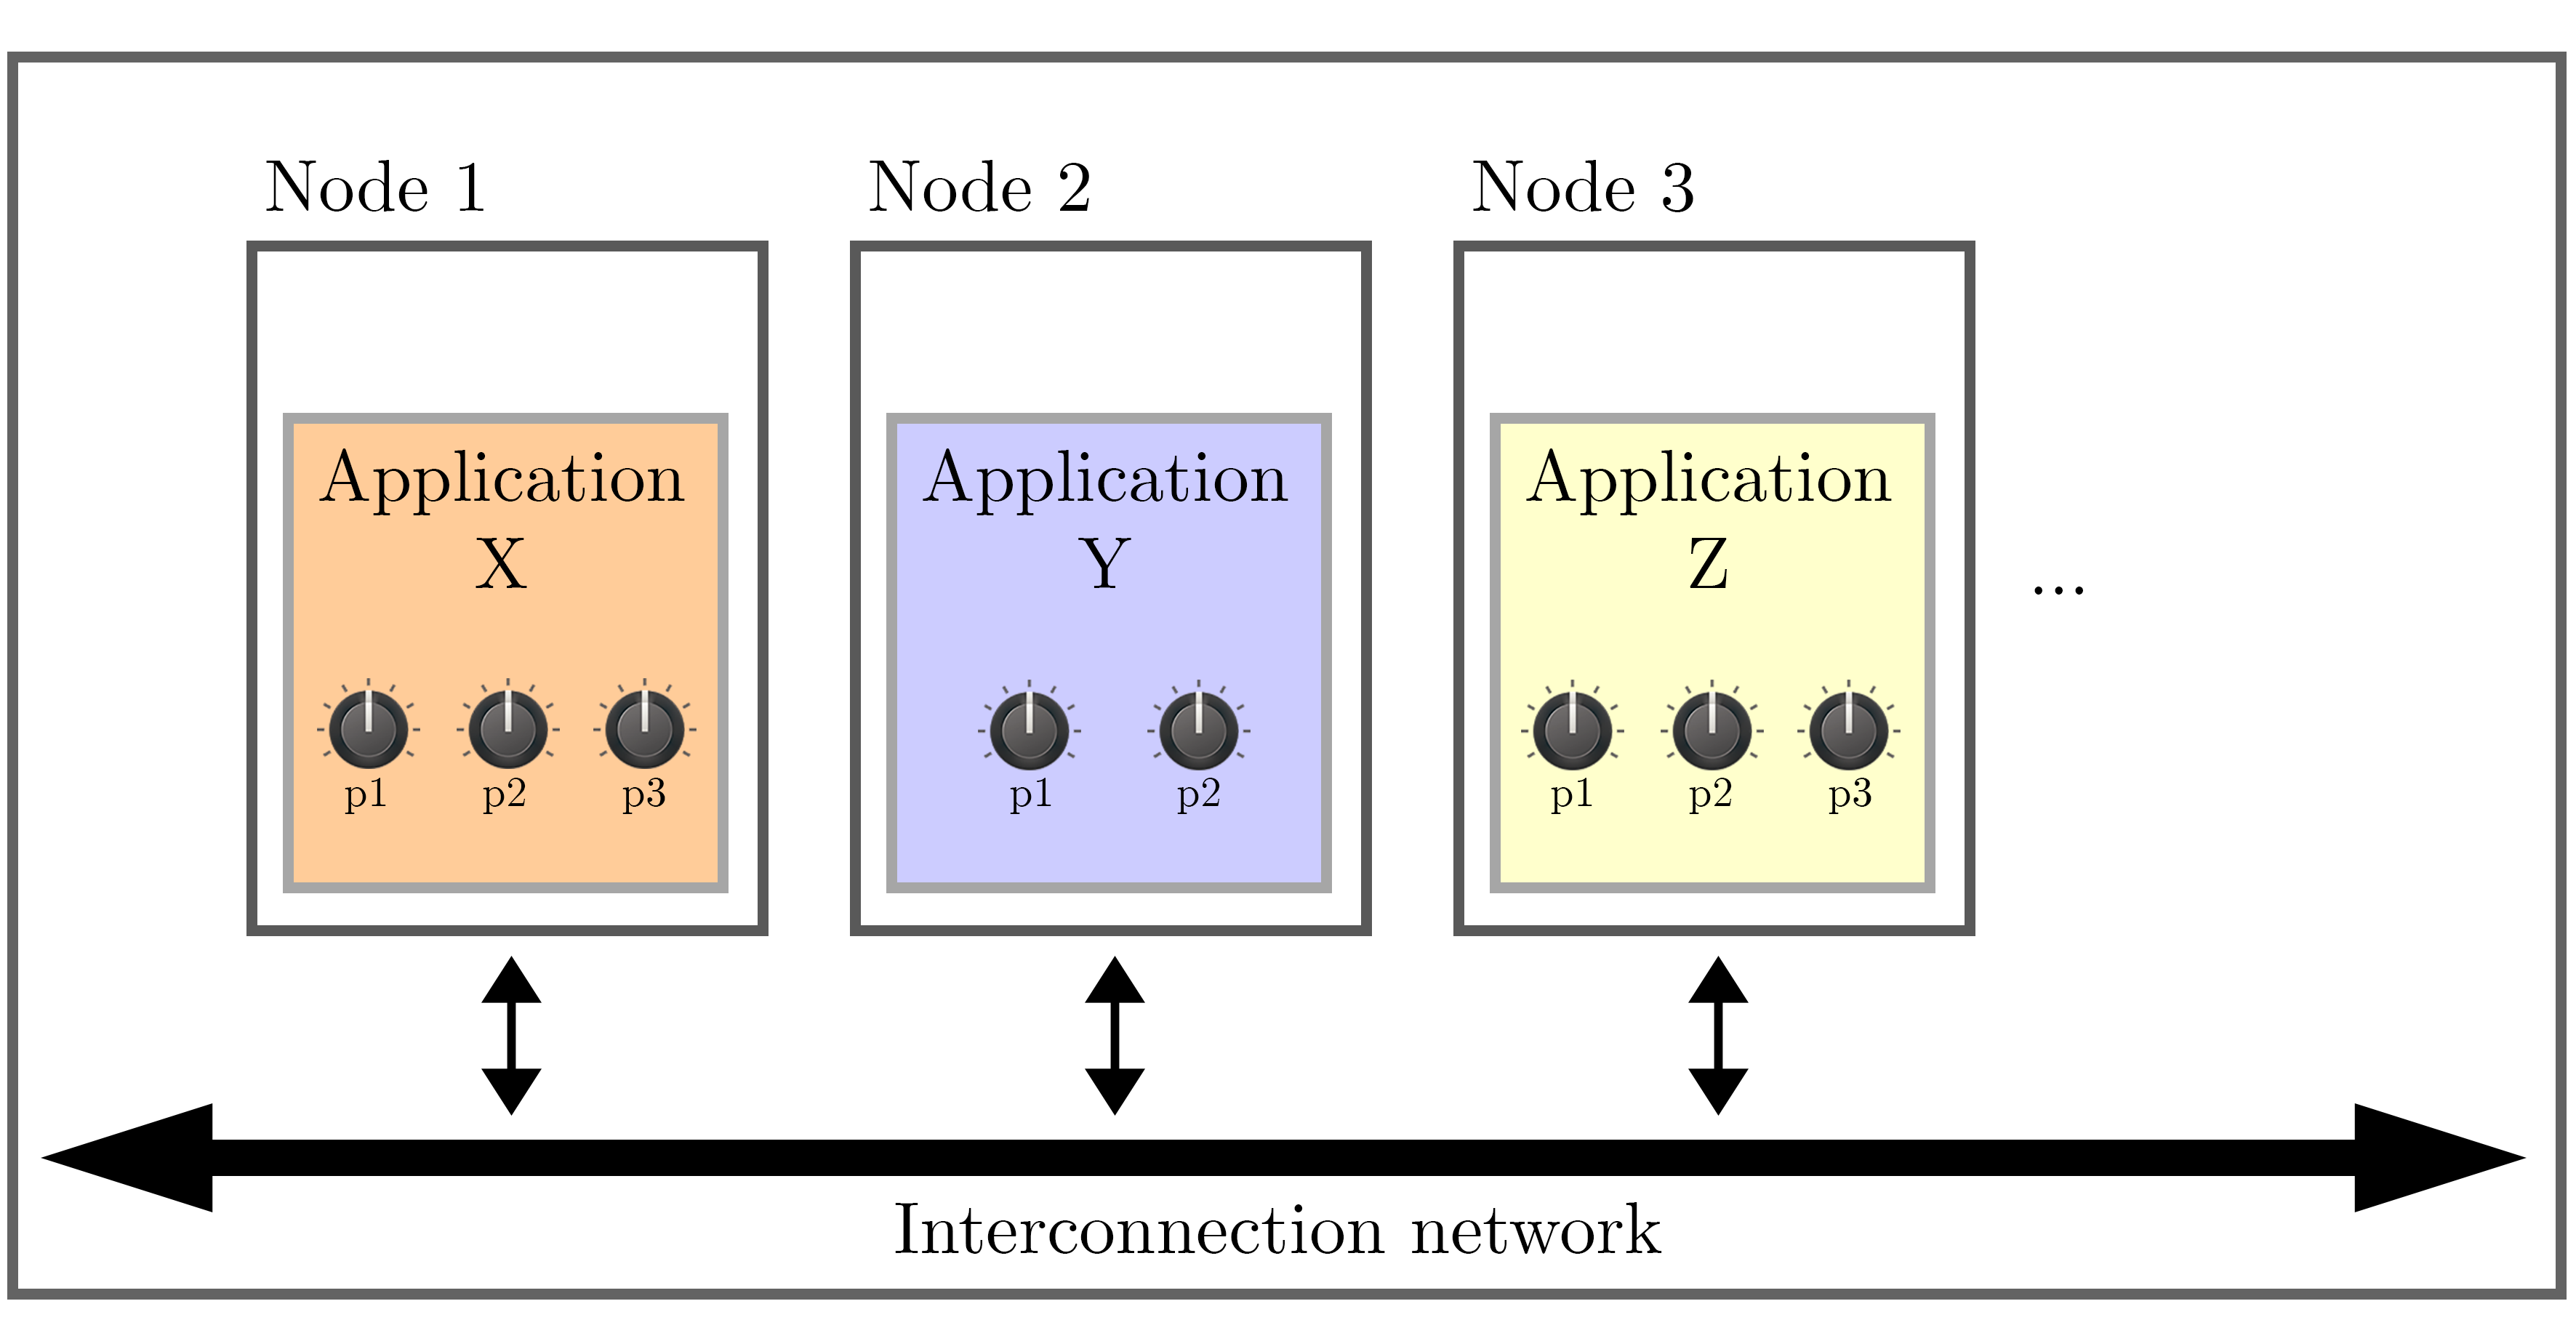
\includegraphics[width = \textwidth]{Apps}
    \caption[Parallel architecture with tunable applications example]{An example of a parallel architecture with three executing tunable applications: application X on node 1 and application Z on node 3 have three knobs, while application Y on node 2 has two knobs}
    \label{fig::appDef}
    
\end{figure}

Very often, High Performance Computing applications expose a large set of parameters, making related Design Space huge and, consequently, unrealistic to explore it in an exhaustive way. In order to choose, from time to time, best program setting with the aim to improve energy efficiency with respect to power consumption and current input data, the concept of Runtime Autotuning is used: a class of online autotuners is able to choose, from time to time, best possible parameter values that fulfill application goals and requirements, starting from a design-time knowledge that gives information about parameter values and corresponding metric of interest values, built off-line. Figure \ref{fig::appAut} shows application Z interconnected with mARGOt \cite{gadioli2015application}, a dynamic autotuner developed by PoliMi research group.

\begin{figure}[H]

    \centering
    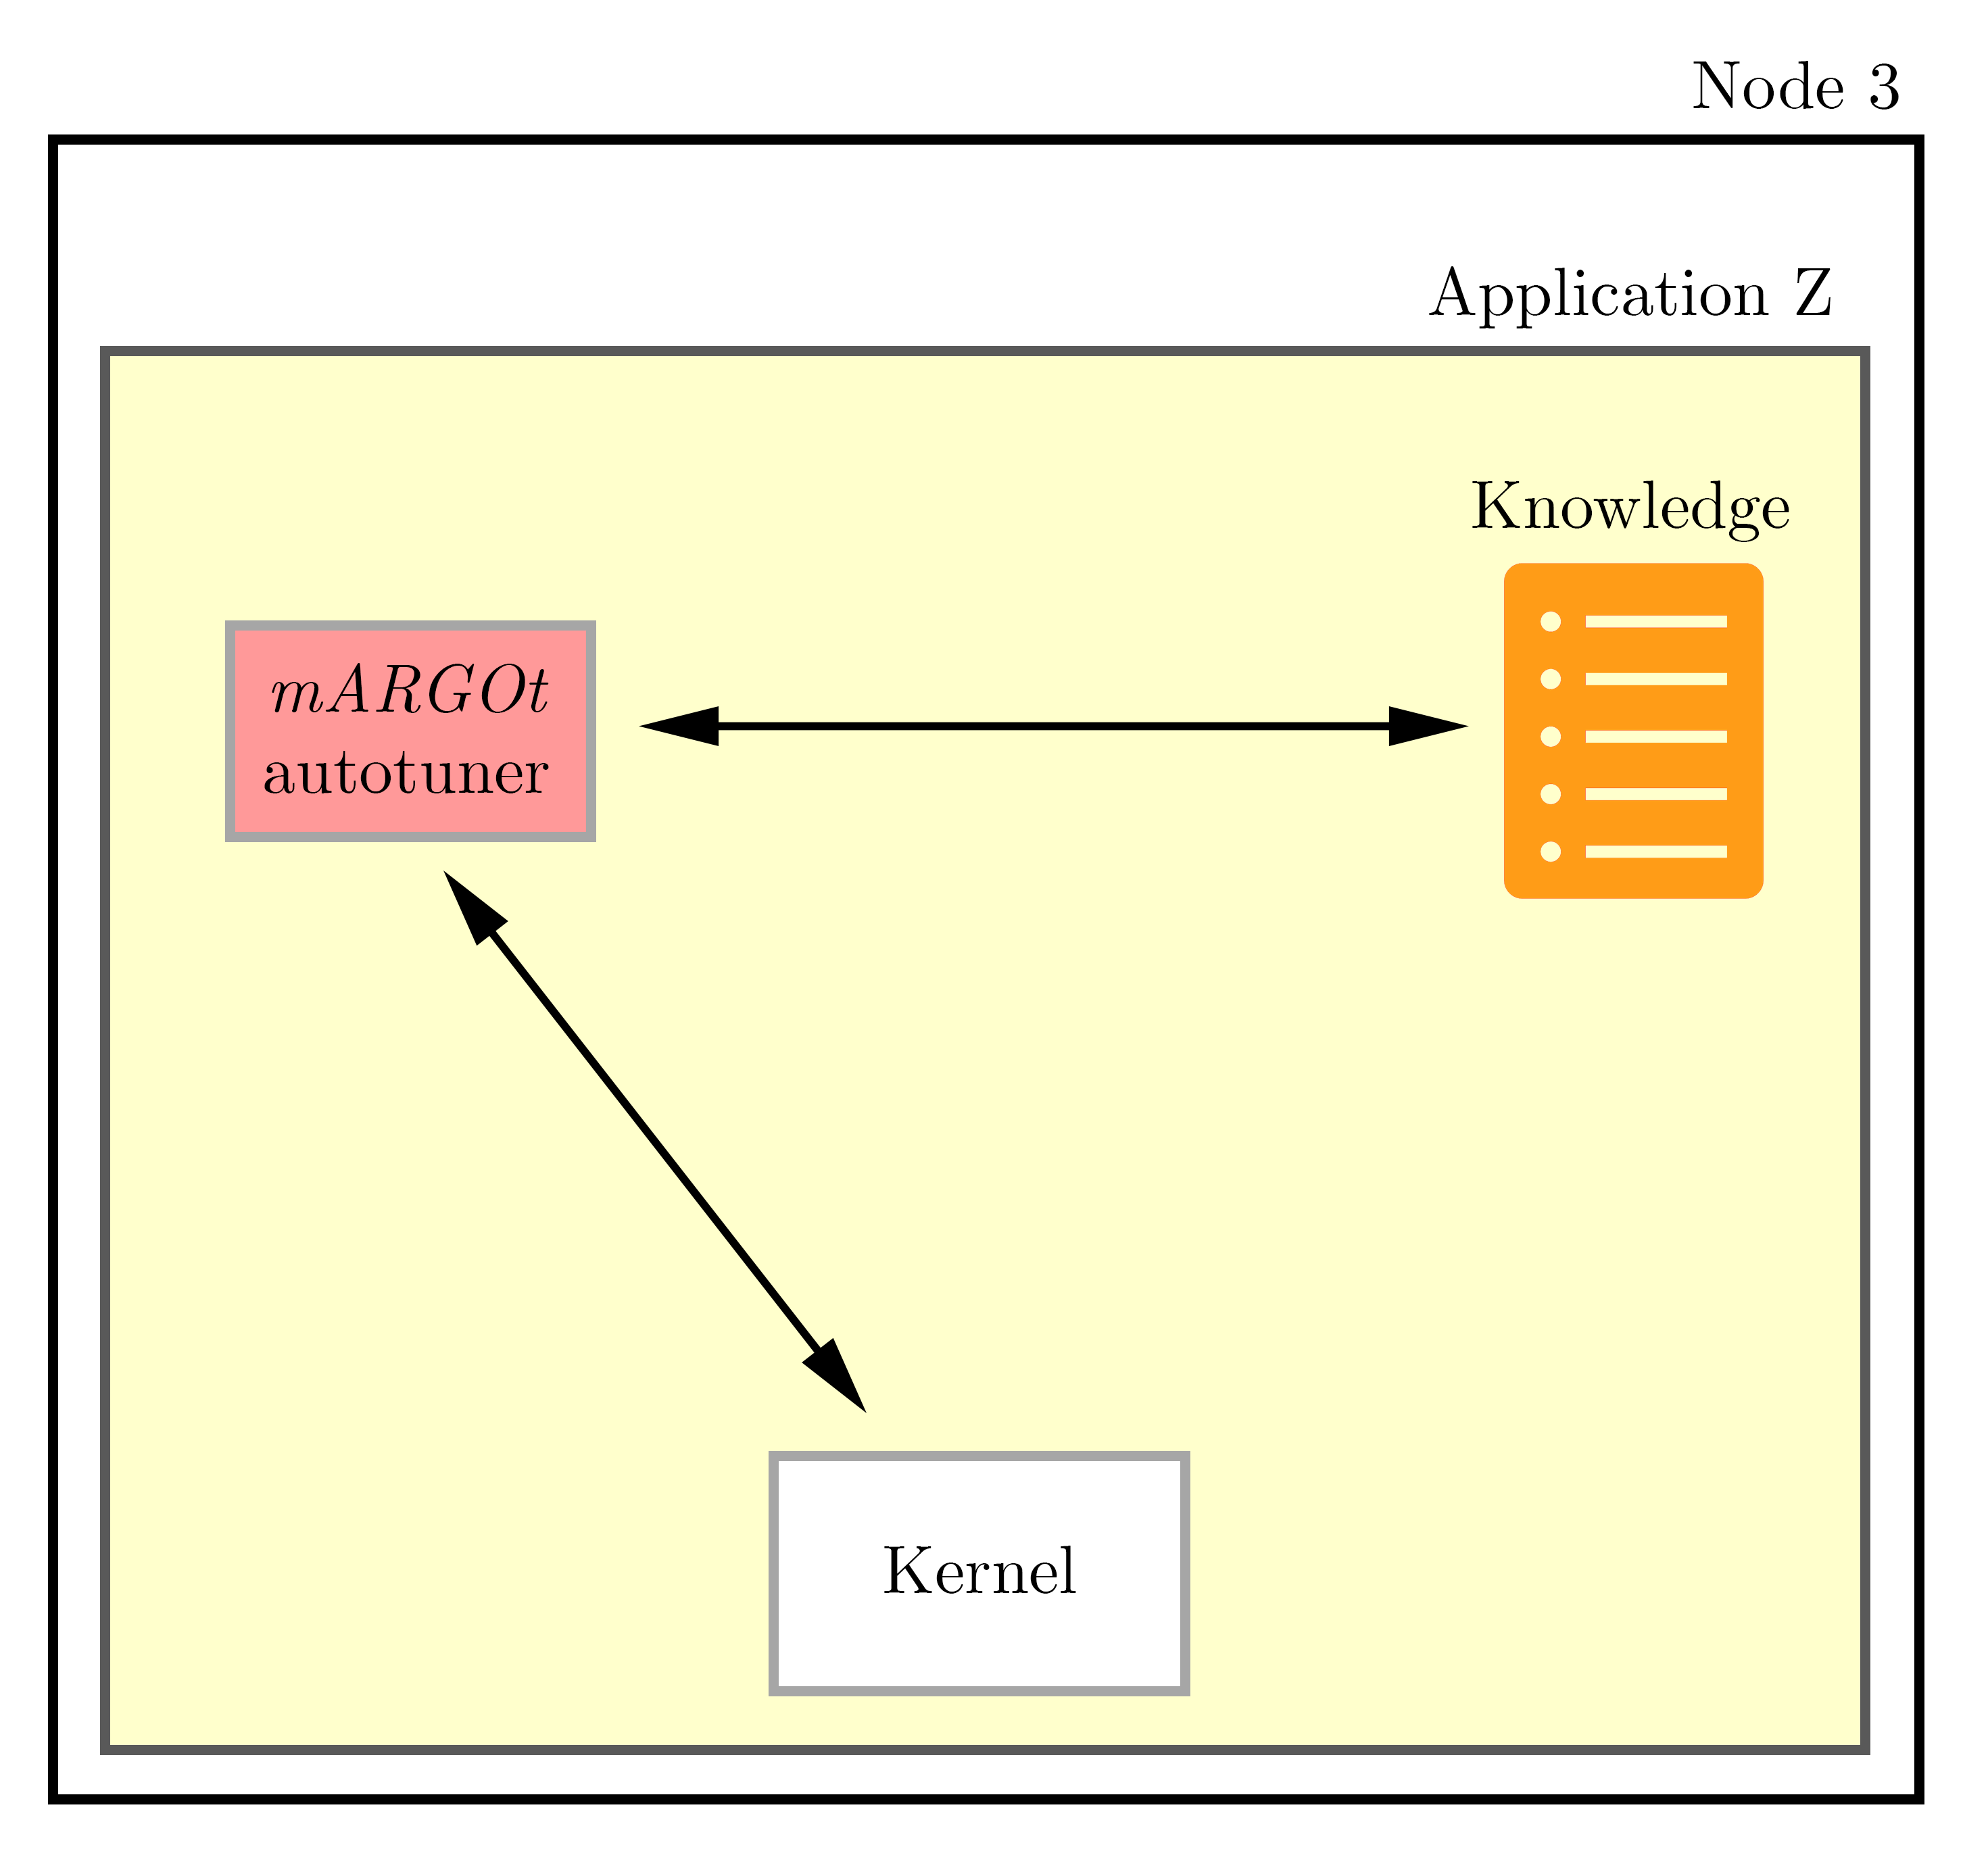
\includegraphics[width = \textwidth]{App_mARGOt}
    \caption{A tunable application Z with the assistance of mARGOt autotuner}
    \label{fig::appAut}
    
\end{figure}

The autotuner needs application knowledge, so there have to be a preceding offline phase (before program start of computation) for profiling. This thesis contributes to avoid this offline step by building, managing and updating application knowledge during execution itself. A local module mainly takes care of properly setting application knowledge, while a remote one manages collected information during execution, in order to predict complete application model. Figure \ref{fig::appAGORA} shows application Z interconnected with Agora and mARGOt autotuner.

\begin{figure}[H]

    \centering
    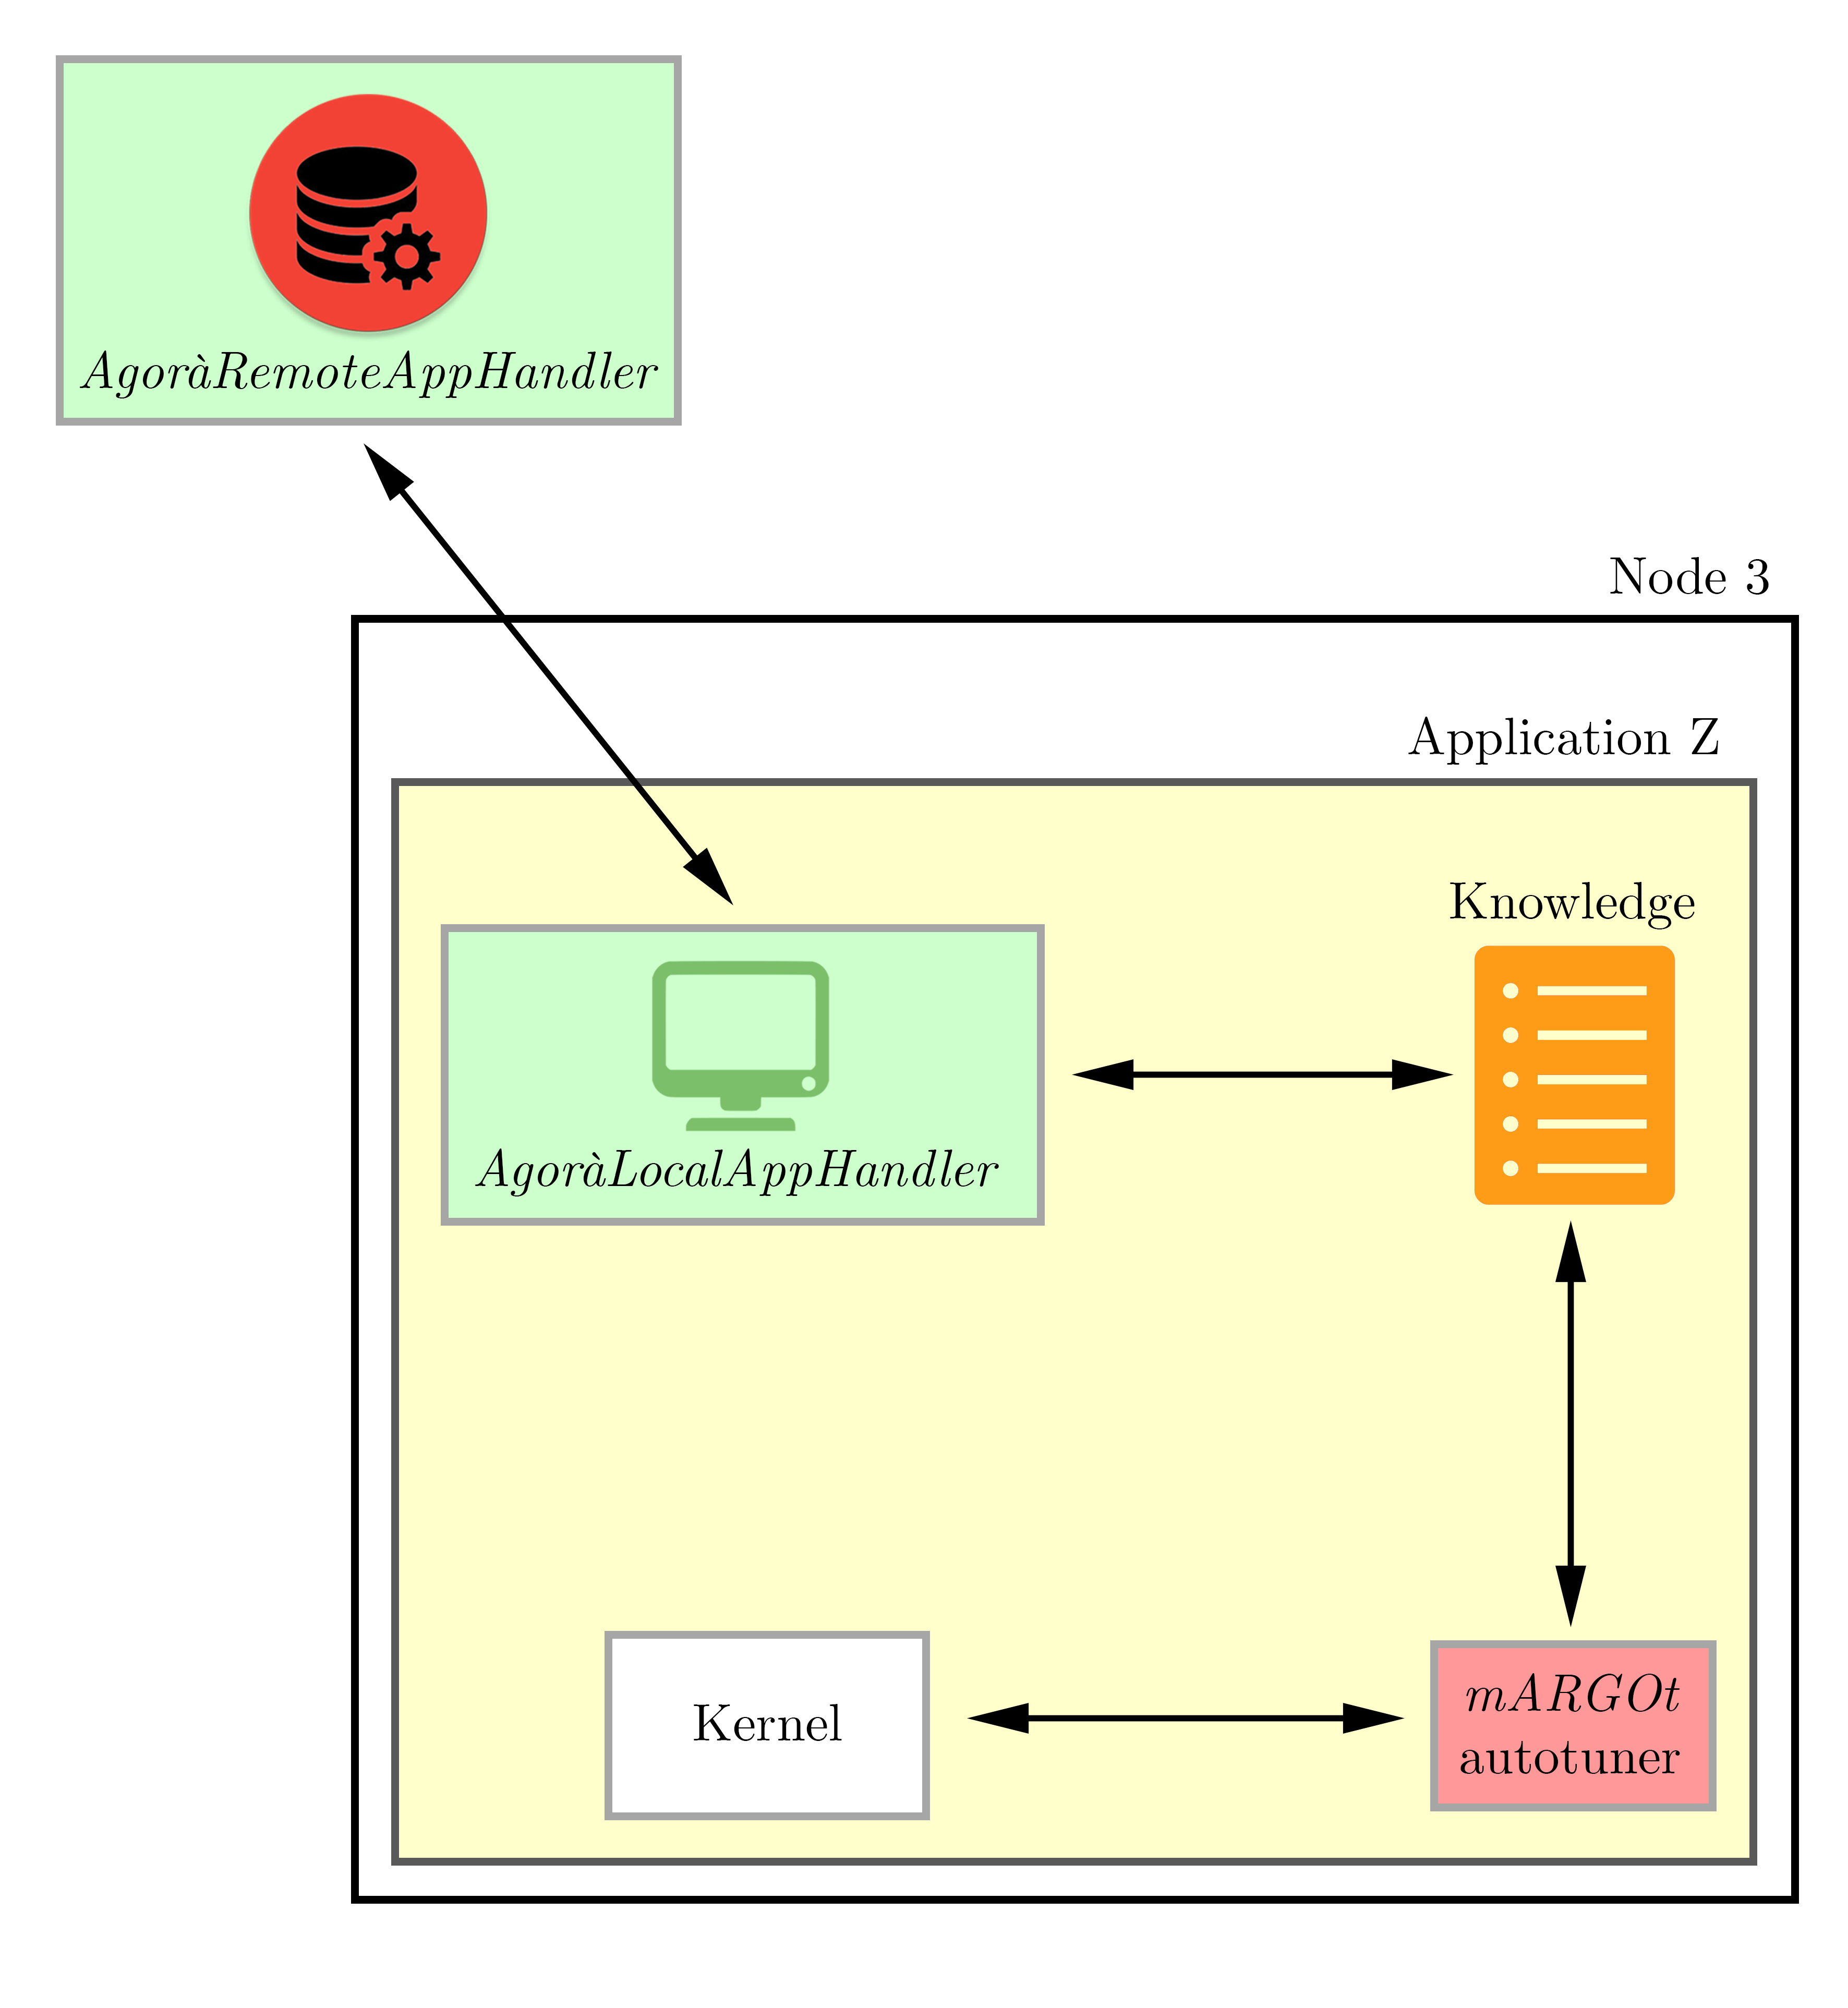
\includegraphics[width = \textwidth]{App_Agora_mARGOt}
    \caption{A tunable application Z with the assistance of Agora and mARGOt autotuner}
    \label{fig::appAGORA}
    
\end{figure}

This thesis focuses on the problem of managing concurrent executed by parallel architecture. Main objective of this work is to initially drive program execution with a subset of parameter configurations taken from their Design Space, in order to gather all metric of interest values associated to them. This list composes the training set for the prediction of application complete model through Machine Learning techniques. Agora can also correctly manage possible features, where a feature is a particular application element than cannot be set up like software knobs, but it contributes to the estimation of complete model. During the DSE phase, feature values are observed like metric values while, during model prediction, they are considered as parameters, so their observations take part to the estimation of metric of interest values.

The typical architecture in which Agora works is parallel, where there are multiple nodes, potentially heterogeneous, that execute applications; the main Agora features are the following:

\begin{enumerate}
    
    \item to drive Design Space Exploration in a distributed way, among all nodes that are running the same program, in order to considerably reduce DSE phase and to speed up overall workflow;
    
    \item to manage multiple kinds of applications, each of them separately organized by a dedicated Agora module that is in charge of all nodes that execute the same program;
    
    \item the out-of-band activity from parallel architecture data streams: computation of Design of Experiments configurations, collection of associated metric of interest values and complete model prediction are done in a separate node with respect to the ones that run applications inside the architecture, while the exchange of information is done using the lightweight MQTT protocol (discussed in Chapter \ref{mqtt});
    
    \item the persistence of generated knowledge: once application complete model is predicted, it is stored so, at any time, it can be reloaded and it is sent to new nodes that start running the same application, without repeating all the workflow through which the complete model has been previously predicted;
    
    \item to recover the cases where a running node crash and to recover the interruption of remote Agora module that has the objective to predict application complete model: if the former situation happens, Agora has to properly handle remaining running nodes; if the latter situation happens, running nodes inside the parallel architecture does not have to stop their execution but they react properly, according to the internal state of their related local Agora module at that moment.

\end{enumerate}

\begin{figure}[H]

    \centering
    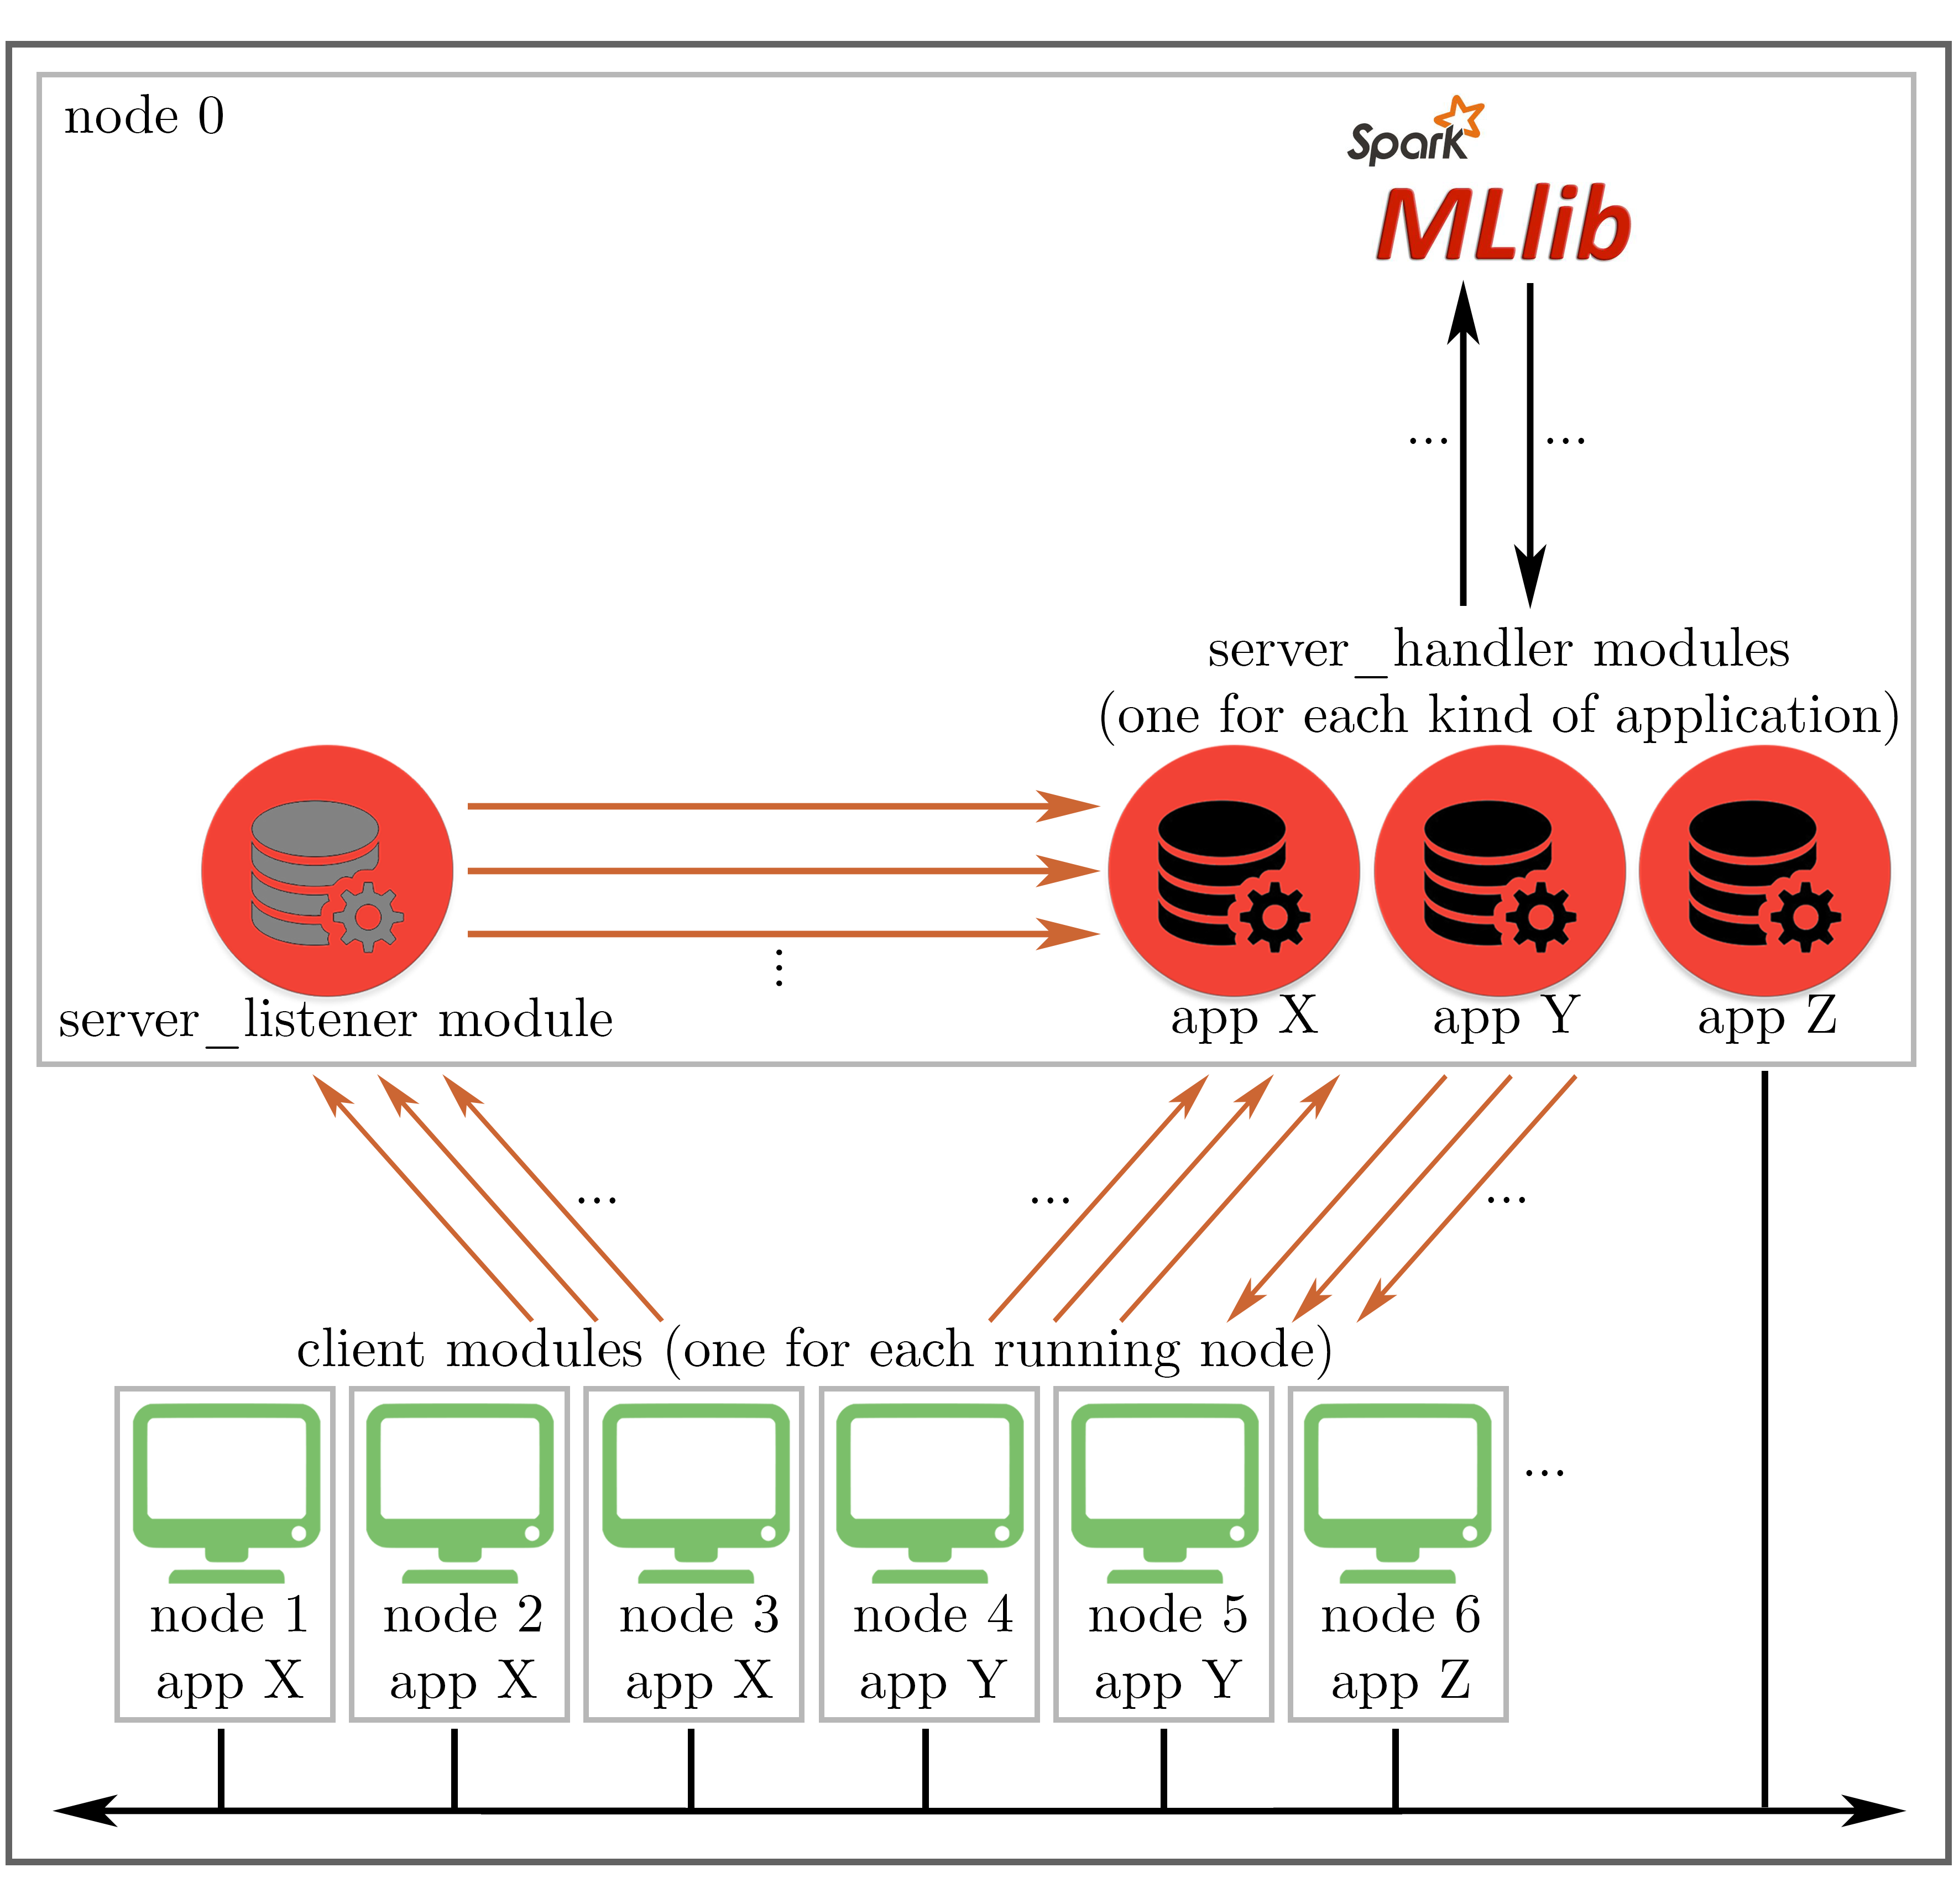
\includegraphics[width = \textwidth]{tesiCris_overall}
    \caption{Agora overview in a parallel architecture}
    \label{fig::tesiCris_overview}
    
\end{figure}

Figure \ref{fig::tesiCris_overview} shows all Agora components and a possible scenario with a parallel architecture in which six nodes are running three different types of tunable applications; for each type of application there exists a dedicated AgoraRemoteAppHandler module that manages it. The orange arrows represent the possible communications among modules, made possible through MQTT subscriptions and publications on predetermined topics.

The main modules of Agora are:

\begin{enumerate}

    \item the \textit{AgoraDispatcher} module, written in Python: it keeps waiting for program arrival, in order to properly manage them;
    
    \item the \textit{AgoraRemoteAppHandler} module, written in Python:
	\begin{itemize}	
		\item [--] it is created by the AgoraDispatcher for each type of application;

		\item [--] it asks for application information such as, for instance, all parameter name and values;

		\item [--] it computes application configurations that compose the Design of Experiments;

		\item [--] it drives Design Space Exploration phase, distributing DoE configurations among all nodes it manages;

		\item [--] it collects parameter values and the observed metrics of interest sent by running programs;

		\item [--] it makes use of Machine Learning techniques in order to build application complete model; finally it sends result to connected nodes.
	\end{itemize}
    
    \item the \textit{AgoraLocalAppHandler} module, written in C++:
	\begin{itemize}
		\item [--] it is set up in every executing program;

		\item [--] it communicates with the autotuner that manages application behavior;

		\item [--] it notifies the existence of related running machine to the AgoraDispatcher module;

		\item [--] it replies to possible information request made by the related AgoraRemoteAppHandler;

		\item [--] during Design Space Exploration phase, it receives configurations from the AgoraRemoteAppHandler module, it sets up program knowledge with this information and, after the application has done computation, it sends back all obtained information, regarding parameter values and associated metric of interest values;

		\item [--] it saves predicted complete model received from the AgoraRemoteAppHandler module, in order to properly update application knowledge with this data.
	\end{itemize}

\end{enumerate}



\section{Workflow}

Principal phases that define framework workflow and the interaction among components are the following:

\begin{enumerate}

    \item application start of execution: when programs start running, related AgoraLocalAppHandler module notifies their existence to the AgoraDispatcher module; if the application is unknown, AgoraDispatcher creates a dedicated AgoraRemoteAppHandler module that is in charge of managing it, otherwise it communicates new node to the corresponding existing AgoraRemoteAppHandler module;
    
    \item Design of Experiments computation: AgoraRemoteAppHandler module computes the subset of configurations, from the entire application Design Space, that compose the Design of Experiments; after that, it is ready to drive Design Space Exploration phase, distributing these configurations to requesting nodes;
    
    \item configuration reception: AgoraLocalAppHandler module updates application knowledge with all the configurations that, from time to time, are sent by the AgoraRemoteAppHandler module; every time program computation is finished, it sends back to the AgoraRemoteAppHandler module a list of values, made by the configuration just used with the observed metrics of interest;
    
    \item application configuration and related metric value collection: A\-go\-ra\-Remote\-App\-Handler module collects all the information it receives from running nodes; when it has all necessary data, it uses Machine Learning techniques in order to predict application complete model, made by all possible configurations associated with predicted metric values;
    
    \item predicted model dispatch: application complete model is sent by AgoraRemoteAppHandler to associated running nodes; related AgoraLocalAppHandler modules update program knowledge with this information, so the dynamic autotuner can set up application knobs with the best configuration that fulfills current goals and requirements.

\end{enumerate}

The interactions among Agora components are implemented in an asynchronous way: program executions are independent from MQTT message exchange and all modules properly react to these events, in order to not condition application workflow and to not steal execution time, making all process as flowing as possible.

\chapter{Agora: proposed framework}\label{agora}

\lettrine{T}{}\textit{his} Chapter shows technical implementation of Agora framework, going into detail of all possible use cases. In the last part, a sketch application explains how AgoraLocalAppHandler module is integrated and how it works.


\section{Introduction}

Agora makes use of the MQTT protocol (\cite{banks2014mqtt}) for the communications among components: it uses Eclipse Paho MQTT Python Client and Eclipse Paho MQTT C Client for managing message exchange (\cite{o2014paho}), while it uses Eclipse Mos\-quitto as broker (\cite{light2013mosquitto}). We take addvantage of the Machine Learning library MLlib by Apache Spark\textsuperscript{TM} (\cite{spark2015apache}) in order to predict application complete models.

Next technical use case implementation makes use of application \textit{Swaptions} as reference, taken from the PARSEC benchmark suite (\cite{bienia2008parsec}). This application is a workload which prices a portfolio of swaptions through Monte Carlo simulations; it has two tunable parameters, the number of threads (variable \textit{num\_threads}, from 1 to 8) and the number of trials for the simulation (variable \textit{num\_trials}, from 100.000 to 1.000.000 with a step of 100.000); observed metrics of interest are: throughput (variable $avg\_throughput$) as the number of priced swaptions per second and error (variable $avg\_error$), computed as:

\[
avg\_error = \dfrac{\sum_{s \in pricedSwaptions} \left\vert StandDevRef(s) - StandDev(s) \right\vert}{\left\vert pricedSwaptions \right\vert}
\]

where $StandDevRef(s)$ is the reference standard deviation for swaption $s$, $StandDev(s)$ is the evaluated one and $pricedSwaptions$ represents the set of swaptions that are priced at each computing cycle; so, metric $avg\_error$ stands for the average of differences between standard deviation of priced swaptions using evaluated configuration with respect to the reference one (standard deviation for 1.000.000 trials).

Agora has been interconnected to mARGOt autotuner (\cite{gadioli2015application}), that exploits design-time knowledge to dynamically adapt application behavior during execution; mARGOt represents this information as a list of Operating Points (OPs): an OP is made by a set of parameter values, also called software knobs, in union with the associated performance (metric of interest values), profiled at design-time; Agora improvement is to build application knowledge at runtime, with an online distributed Design Space Exploration phase in which a subset of OPs are collected, in order to predict the complete model, made by the entire Operating Point list.

Agora could work in union with other autotuners that, using application knowledge in terms of configurations and associated performance, have the capability to dynamically adapt application behavior during execution.










\section{Use case implementation}





\subsection{AgoraRemoteDispatcher module creation}

The starting point is the creation of the AgoraRemoteDispatcher module, that is in charge of managing the arrival of applications; it connects to the MQTT broker and it subscribes to topic "agora/apps" (Figure \ref{fig::dispSub}).

\begin{figure}[ht]

    \centering
    
\includegraphics[width = \textwidth]{server_listener_subscription}
    \caption{AgoraRemoteDispatcher subscription}

    \label{fig::dispSub}
    
\end{figure}





\subsection{Application arrival}

An application can be already known by the Agora\-Remote\-Dis\-patch\-er module or a program is executed by a machine for the first time. We define \textit{known} application a program that is already supervised by an AgoraRemoteAppHandler module, while \textit{unknown} application a program that does not have a dedicated AgoraRemoteAppHandler module.

\subsubsection{Unknown application}

A node starts running a program; the related AgoraLocalAppHandler module notifies this event, publishing on topic "agora\slash{}apps" a string composed of application name and machine hostname plus Process IDentifier (PID), with format "\textit{[appName] [hostname]\_[PID]}", so that AgoraLocalAppHandler module can be univocally recognized in the future; the message is received by Agora\-Remote\-Dispatcher, that creates a dedicated AgoraRemoteAppHandler module for this application (Figure \ref{fig::unk}).

\begin{figure}[hb]

    \centering
    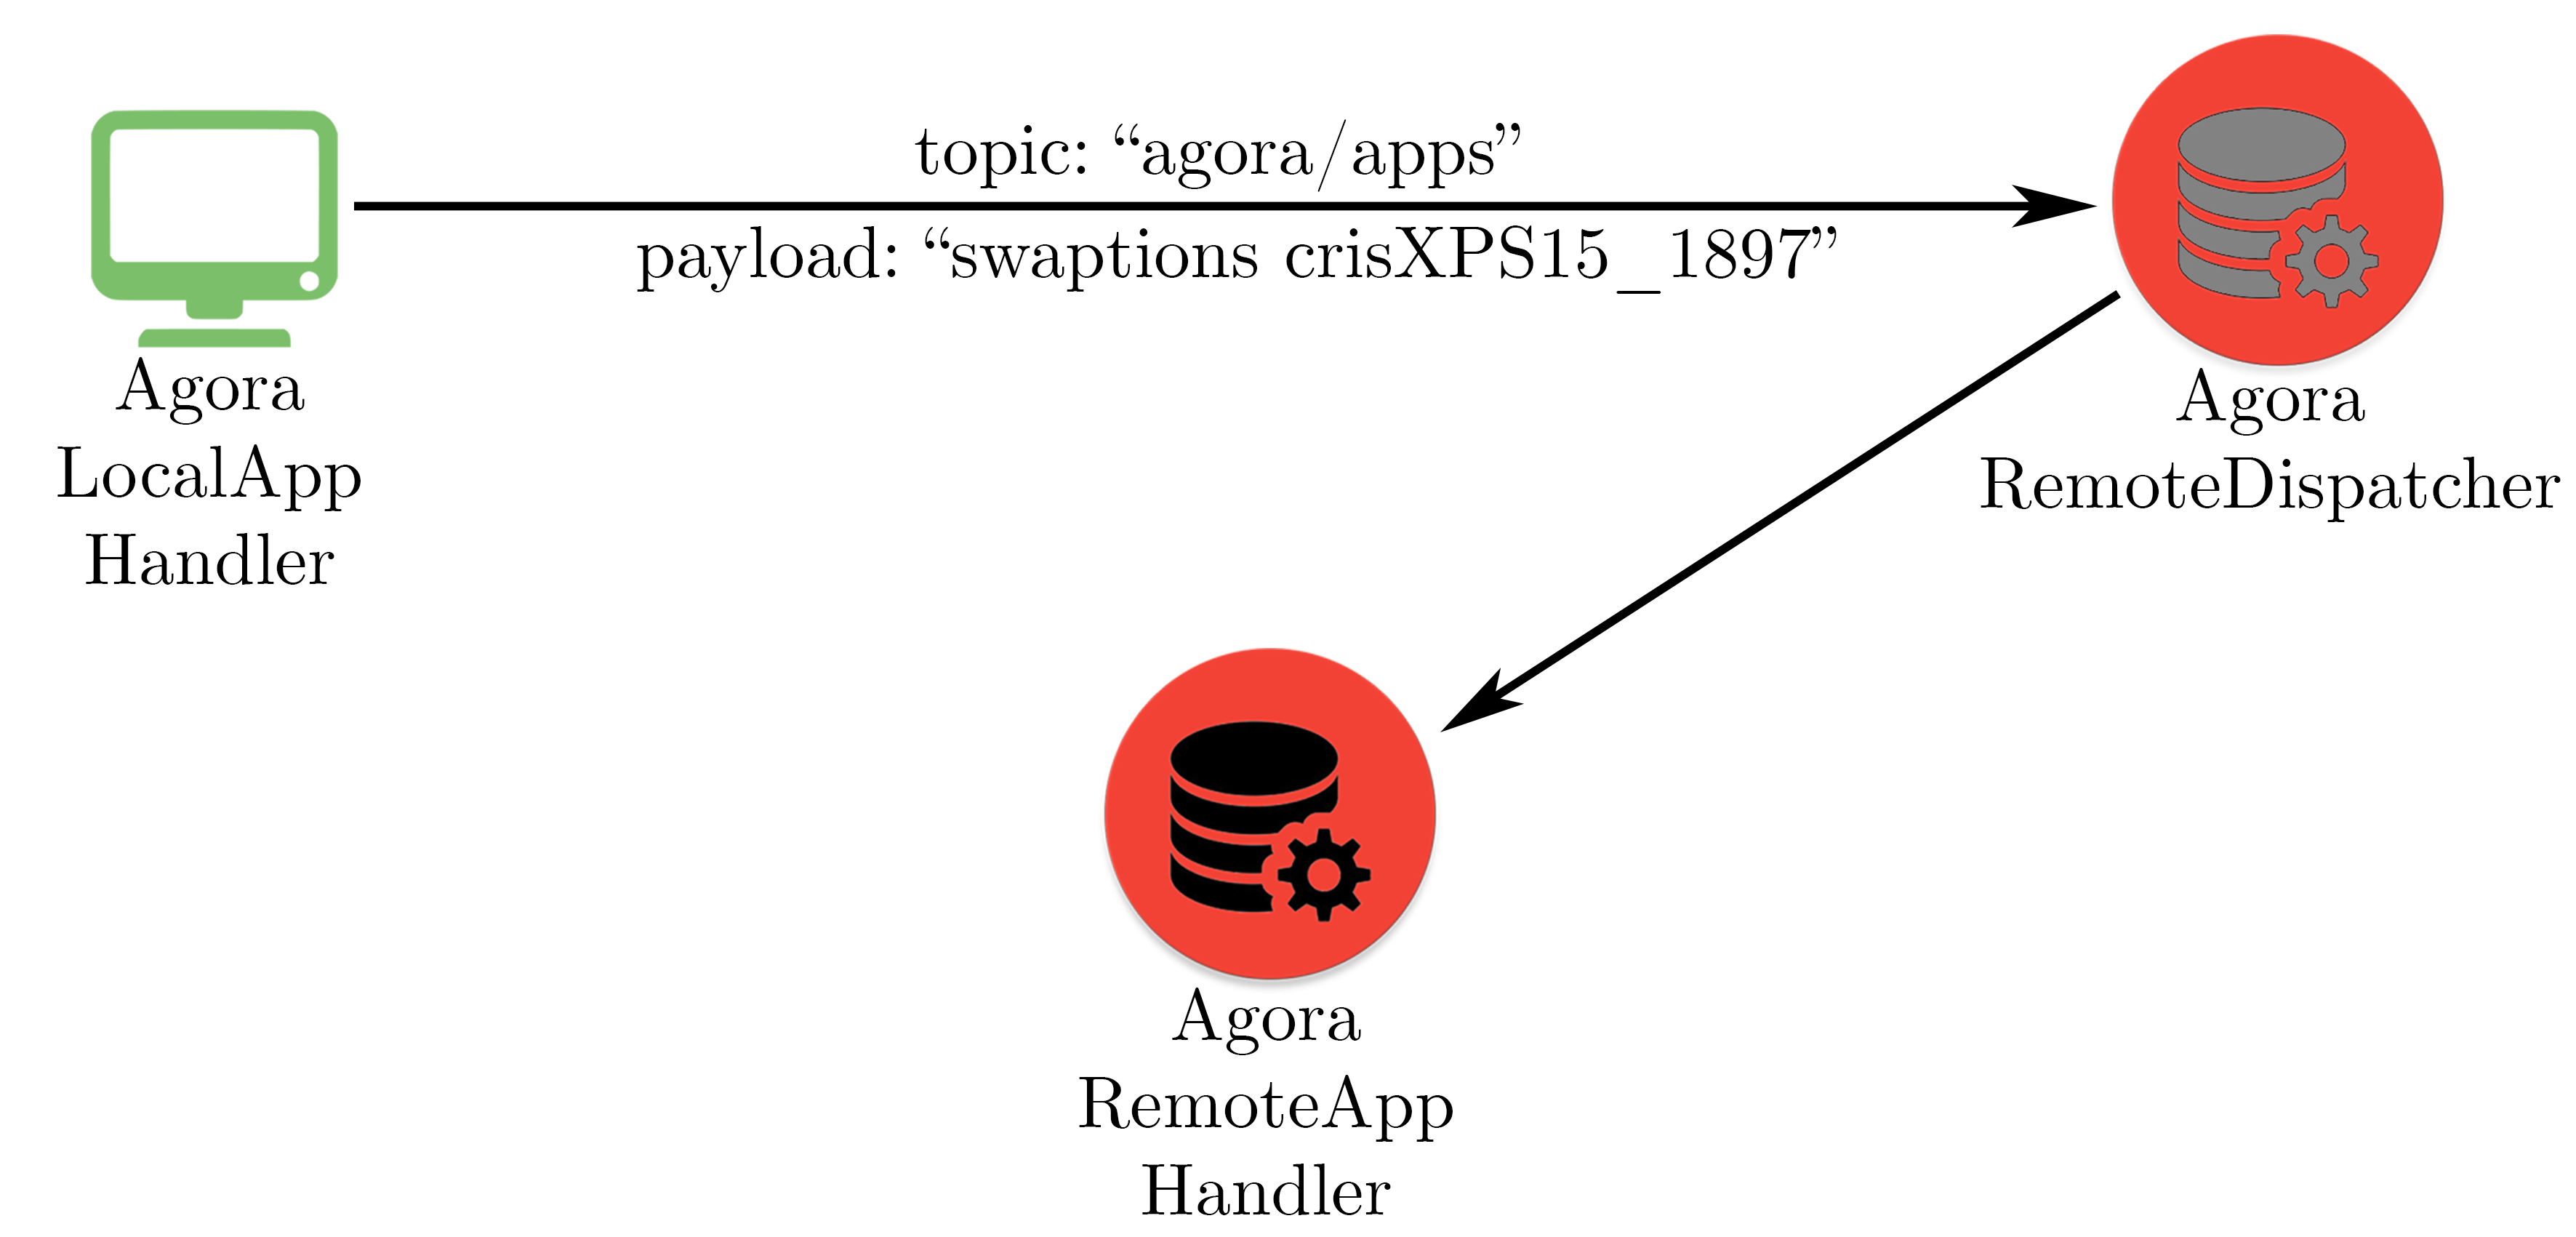
\includegraphics[width = \textwidth]{new_unknown}
    \caption[New unknown application arrival example]{New unknown application arrival example; a dedicated AgoraRemoteAppHandler module is created by AgoraRemoteDispatcher}

    \label{fig::unk}
    
\end{figure}

At the beginning, the Agora\-Local\-App\-Handler module subscribes to some topics that are needed to receive communications from the related Agora\-Remote\-App\-Handler (Figure \ref{fig::localSubs}):

\begin{enumerate}

    \item "agora/\textit{[appName]}", in order to understand if AgoraRemoteAppHandler has asked application information and, therefore, to reply (see \ref{req_info}); this topic is also used to understand if Agora\-Remote\-App\-Handler has crashed and, so, to react properly (see \ref{handler_disc});
    
    \item "agora/\textit{[appName]}/\textit{[hostname]\_[PID]}/conf", in order to receive configurations from AgoraRemoteAppHandler during Design Space Exploration phase (see \ref{dse_conf});
    
    \item "agora/\textit{[appName]}/\textit{[hostname]\_[PID]}/model", in order to receive a partial OP list (see \ref{DoEModelSend}) and the complete predicted model from AgoraRemoteAppHandler (see \ref{modelSend}).

\end{enumerate}

\begin{figure}[t]

    \centering
    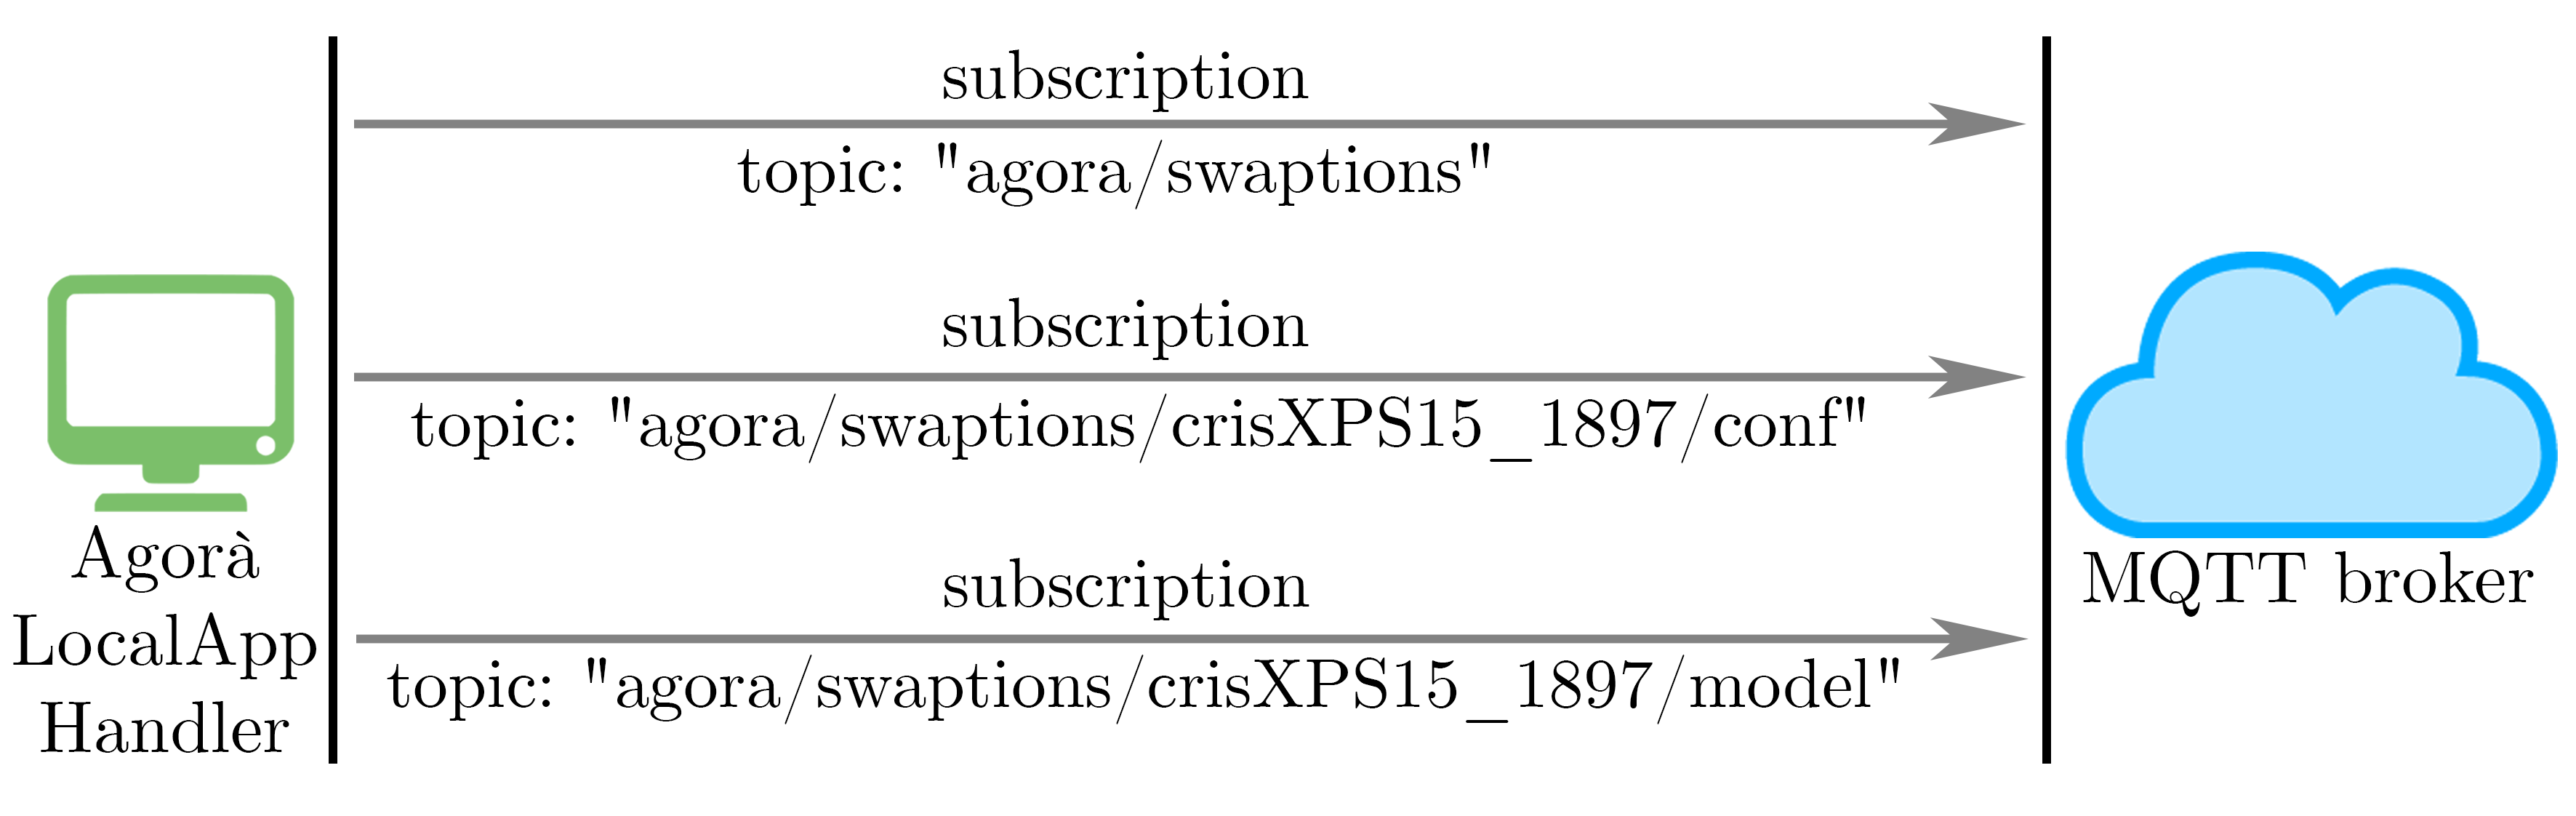
\includegraphics[width = \textwidth]{client_subs}
    \caption{AgoraLocalAppHandler MQTT subscriptions example}

    \label{fig::localSubs}
    
\end{figure}

The AgoraRemoteAppHandler module subscribes to some topics in order to manage correctly all various situations that happens (Figure \ref{fig::remotSubs}):

\begin{enumerate}

    \item "agora/\textit{[appName]}/newHostpid", in order to manage the hypothetical notification of other AgoraLocalAppHandler modules that are supervising the same application (see \ref{knownApp});
    
    \item "agora/\textit{[appName]}/req", in order to manage all the requests made by AgoraLocalAppHandler modules during program execution (see \ref{clientReq});
    
    \item "agora/\textit{[appName]}/info/\#", in order to receive all available application information, such as parameter name and values (see \ref{client_info}); real topic is "agora\slash{}\textit{[appName]}\slash{}info\slash{}\textit{[host\-name]\_ [PID]}" (see MQTT multi-level wildcard, \ref{mqtt}), therefore Agora\-Remote\-App\-Handler can store the ID of the node that is sending application information, in order to react properly to node possible crash during this phase (see \ref{client_disc});
    
    \item "agora/\textit{[appName]}/disconnection", in order to correctly react to a possible node disconnection (see \ref{client_disc});
    
    \item "agora/\textit{[appName]}/OPs", in order to receive Operating Points from AgoraLocalAppHandler modules during Design Space Exploration phase (see \ref{opSend}).

\end{enumerate}

\begin{figure}[t]

    \centering
    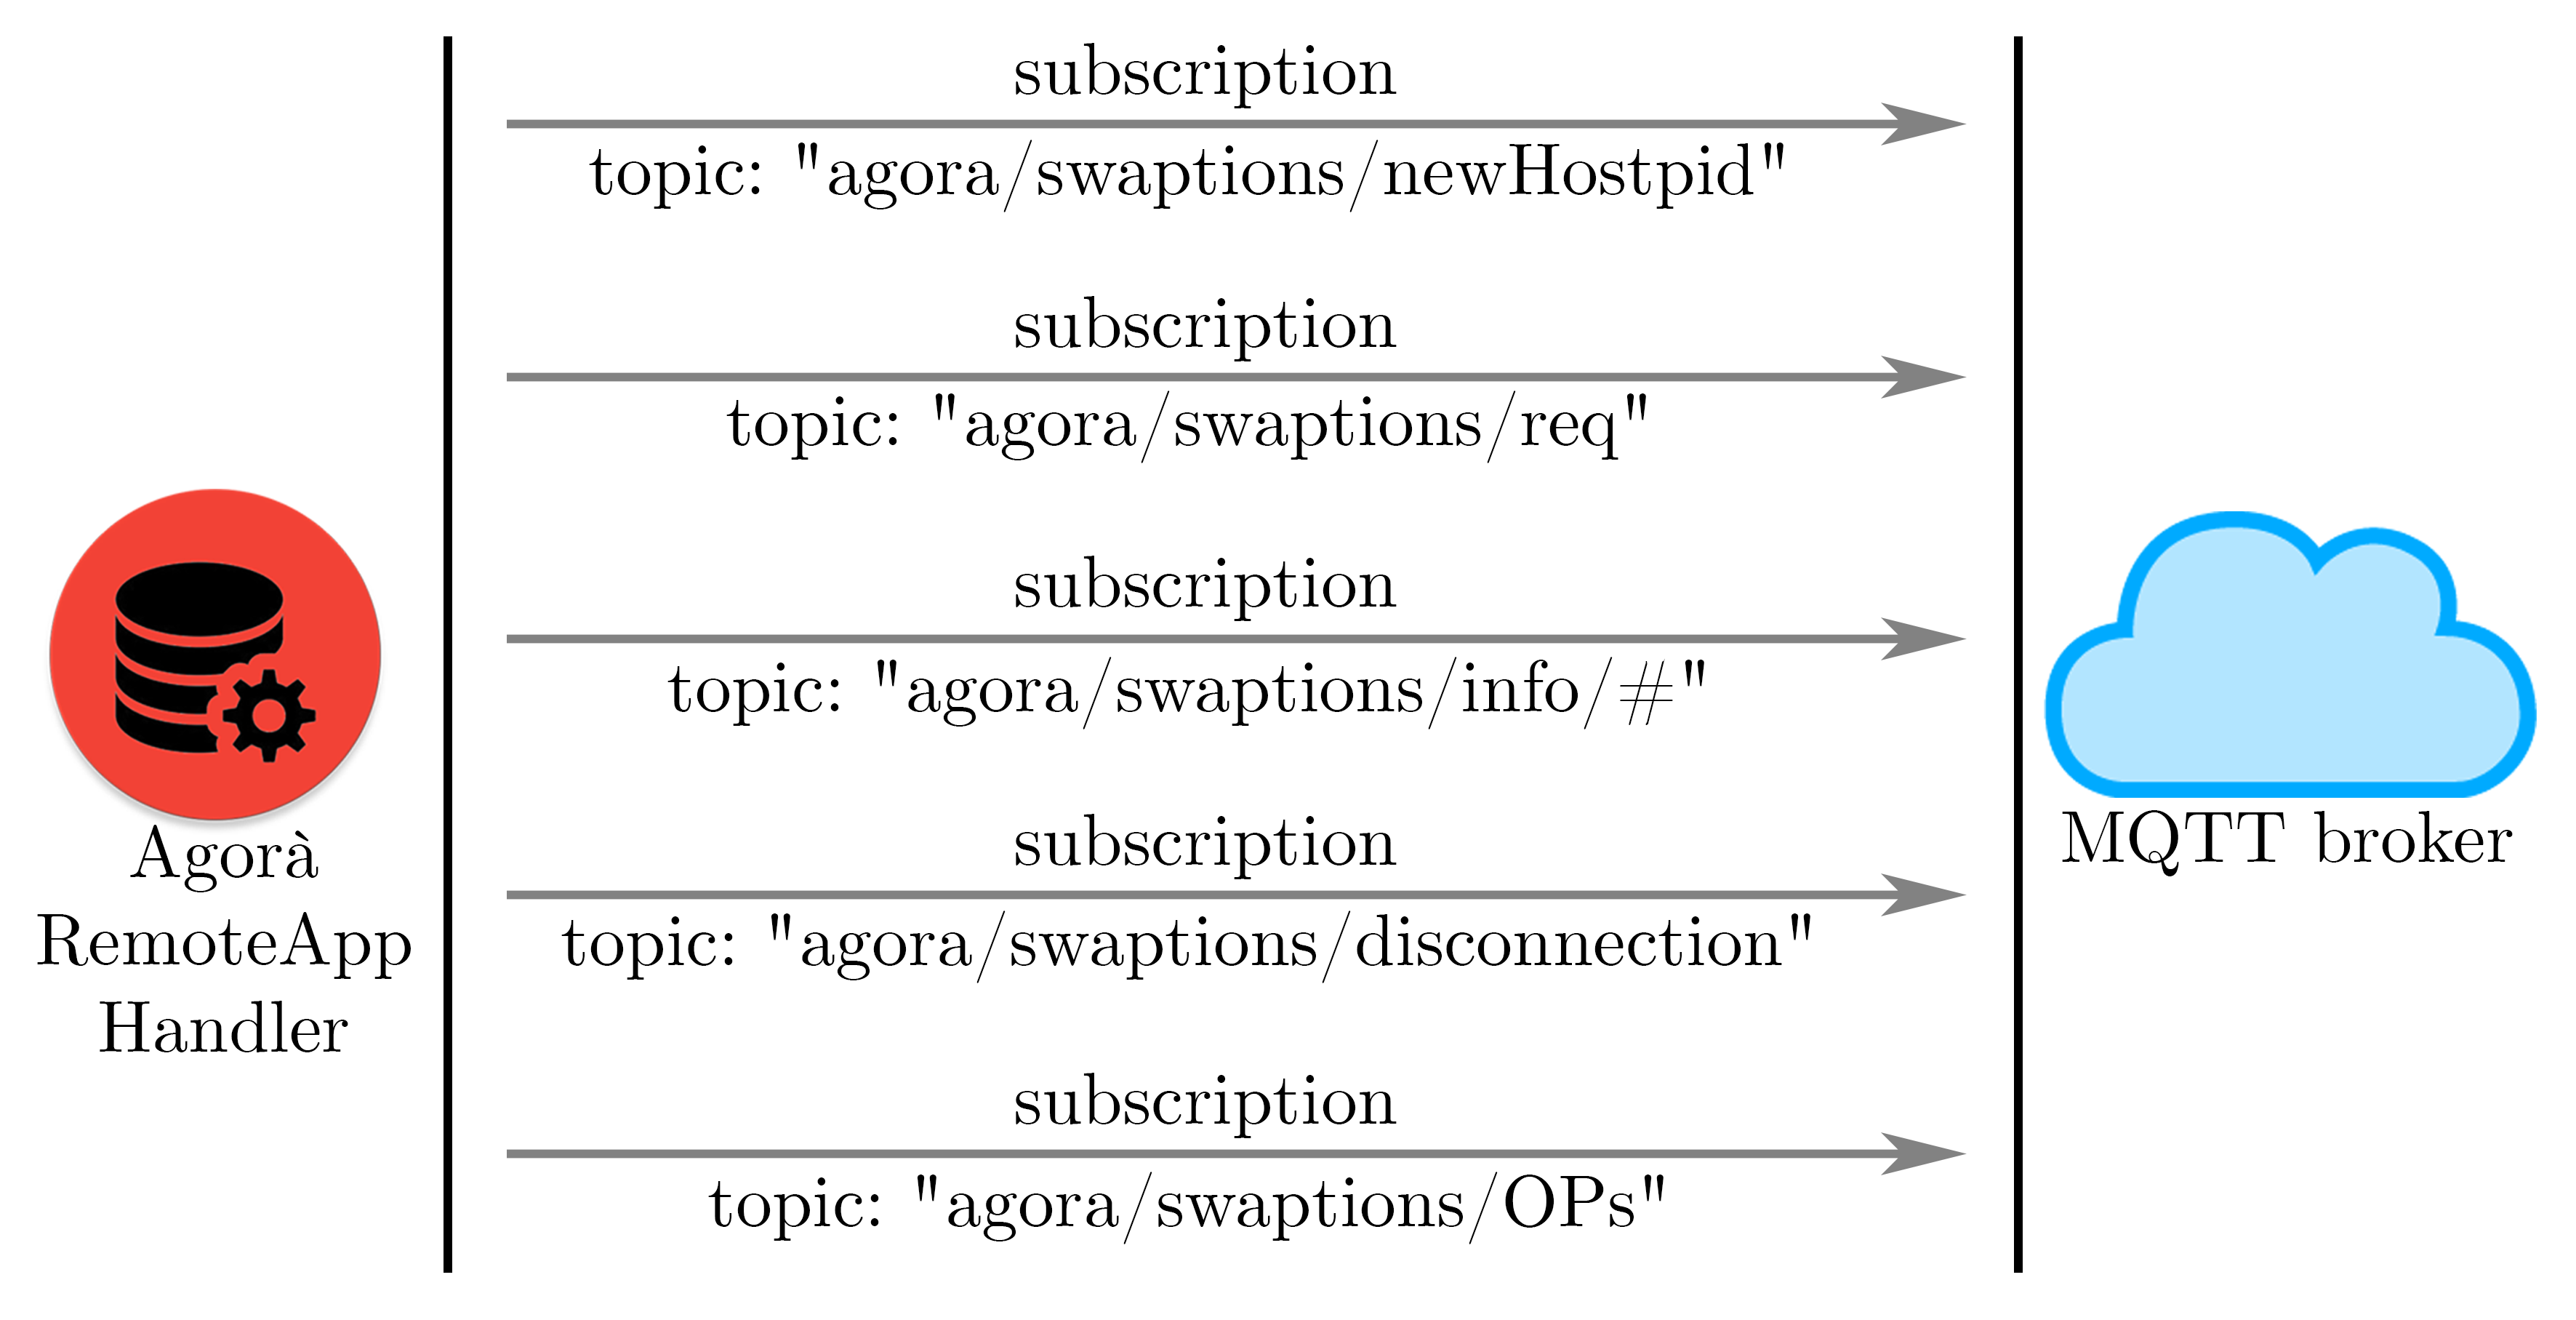
\includegraphics[width = \textwidth]{handler_subs}
    \caption{AgoraRemoteAppHandler MQTT subscriptions example}

    \label{fig::remotSubs}
    
\end{figure}


\subsubsection{Known application}\label{knownApp}

When the AgoraRemoteDispatcher module is informed that a new node has started running an application but there exist already an AgoraRemoteAppHandler that is managing that program, it publishes on topic "agora\slash{}\textit{[app\-Name]}\slash{}newHostpid" the new machine hostname plus PID, so that the corresponding Agora\-Remote\-App\-Handler module can add the node to the pool of machines that are running the application it is supervising (Figure \ref{fig::knownApp}).

\begin{figure}[ht]

    \centering
    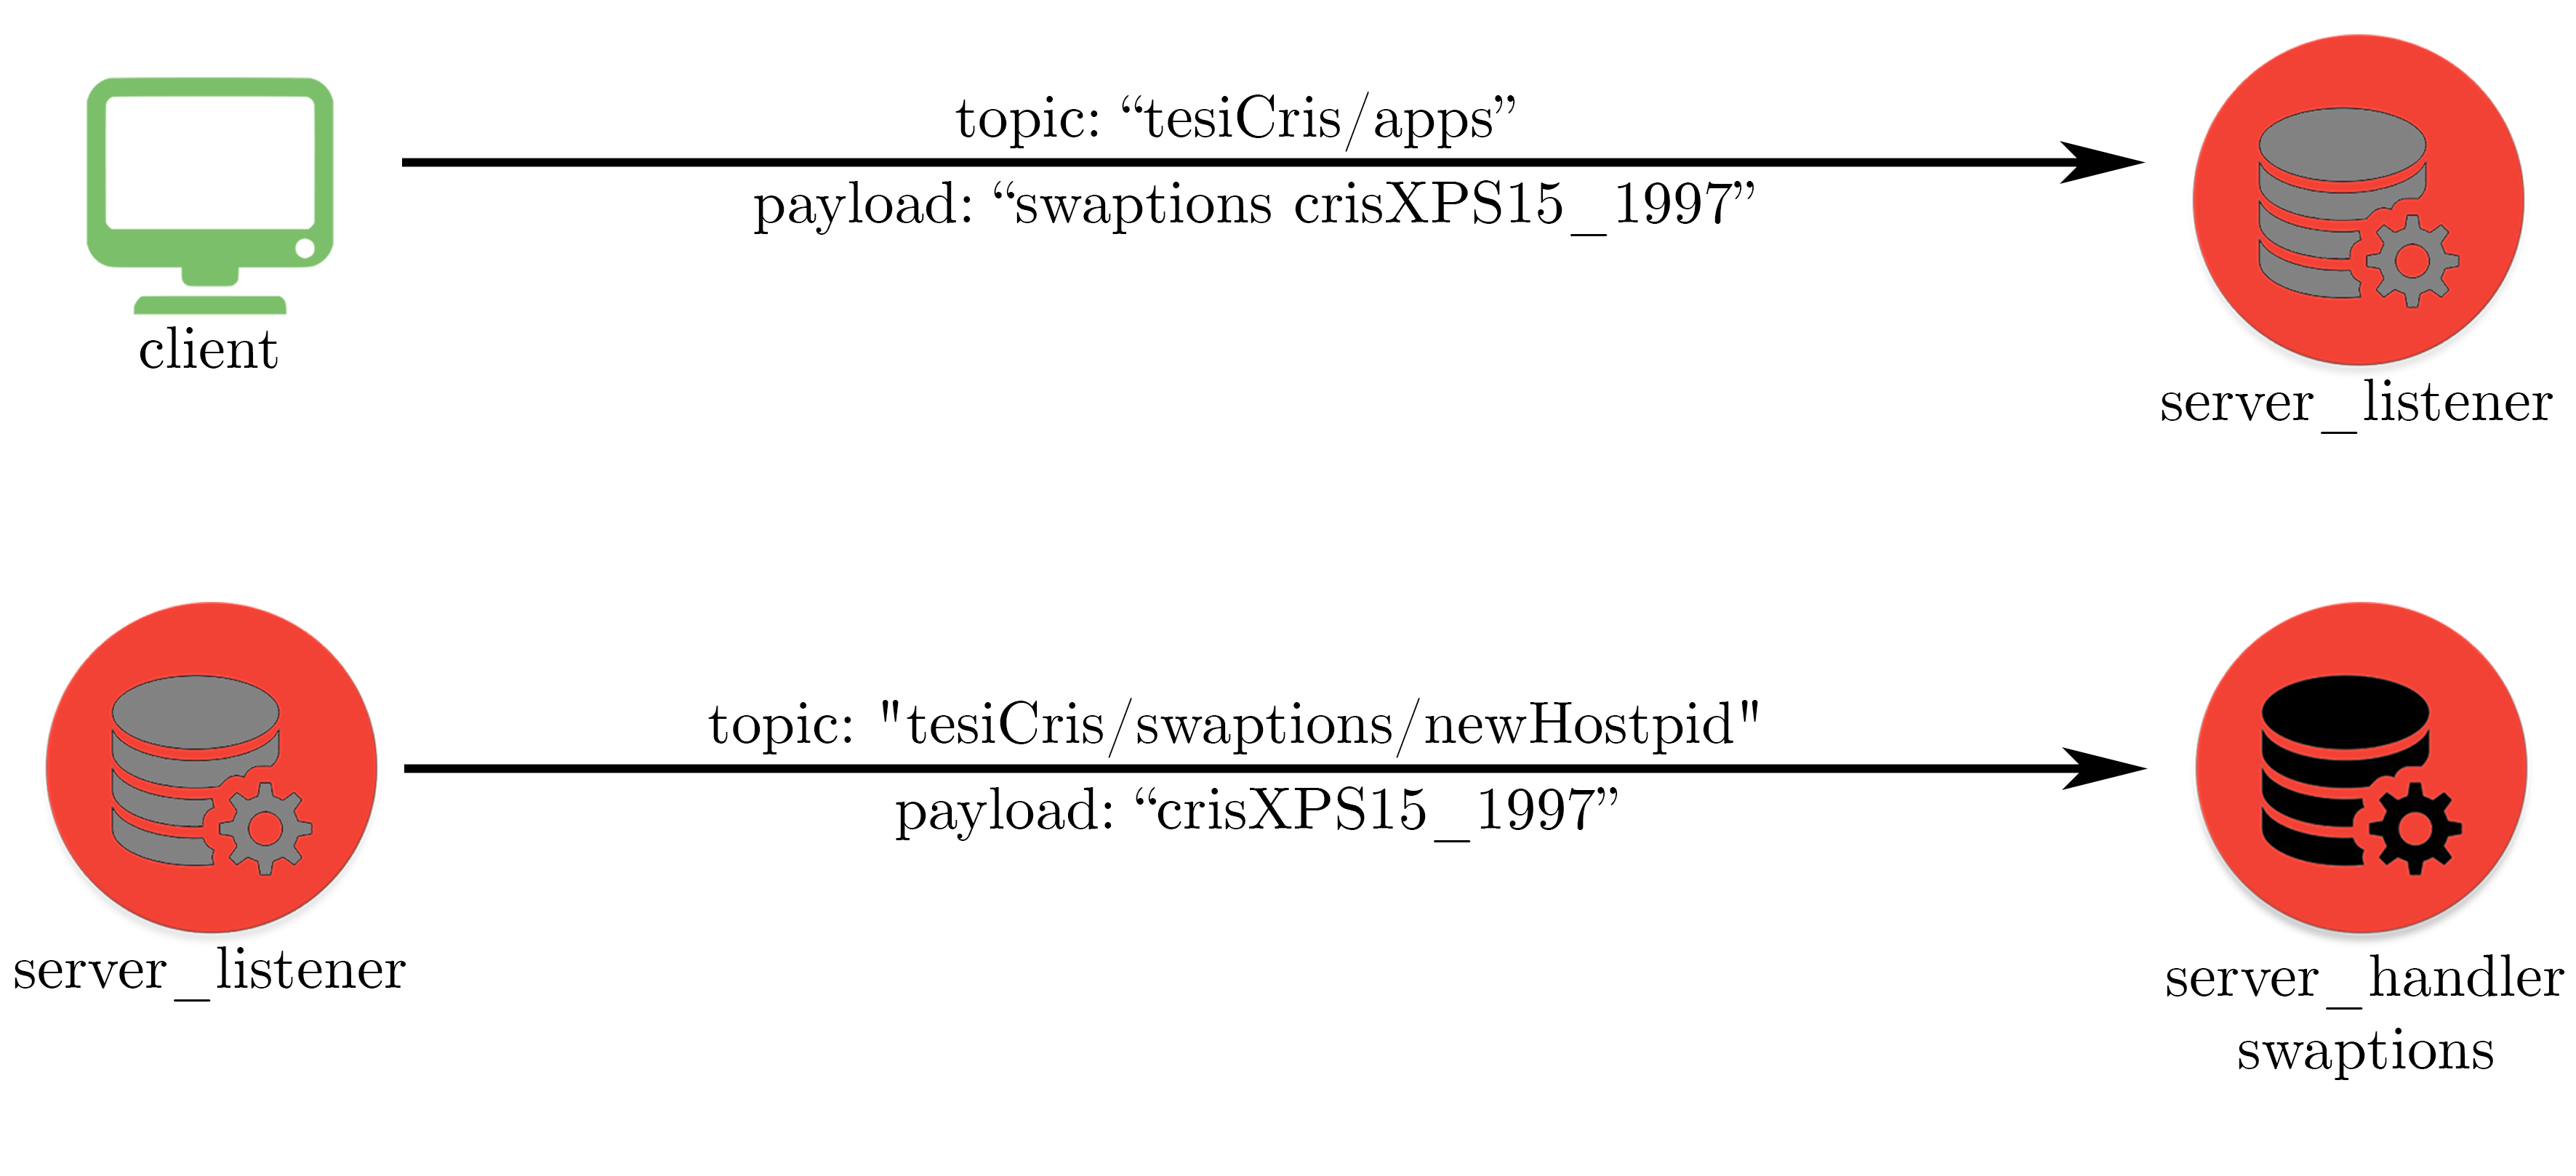
\includegraphics[width = \textwidth]{new_known}
    \caption[New known application arrival example]{New known application arrival example; node ID is sent by AgoraRemoteDispatcher to the corresponding AgoraRemoteAppHandler module}

    \label{fig::knownApp}
    
\end{figure}





\subsection{AgoraLocalAppHandler request}\label{clientReq}

At each predetermined time interval, AgoraLocalAppHandler modules make a request to the related AgoraRemoteAppHandler, publishing their hostname plus PID on topic "agora/\textit{[appName]}/req" (Figure \ref{fig::localReq}).

\begin{figure}[hb]

    \centering
    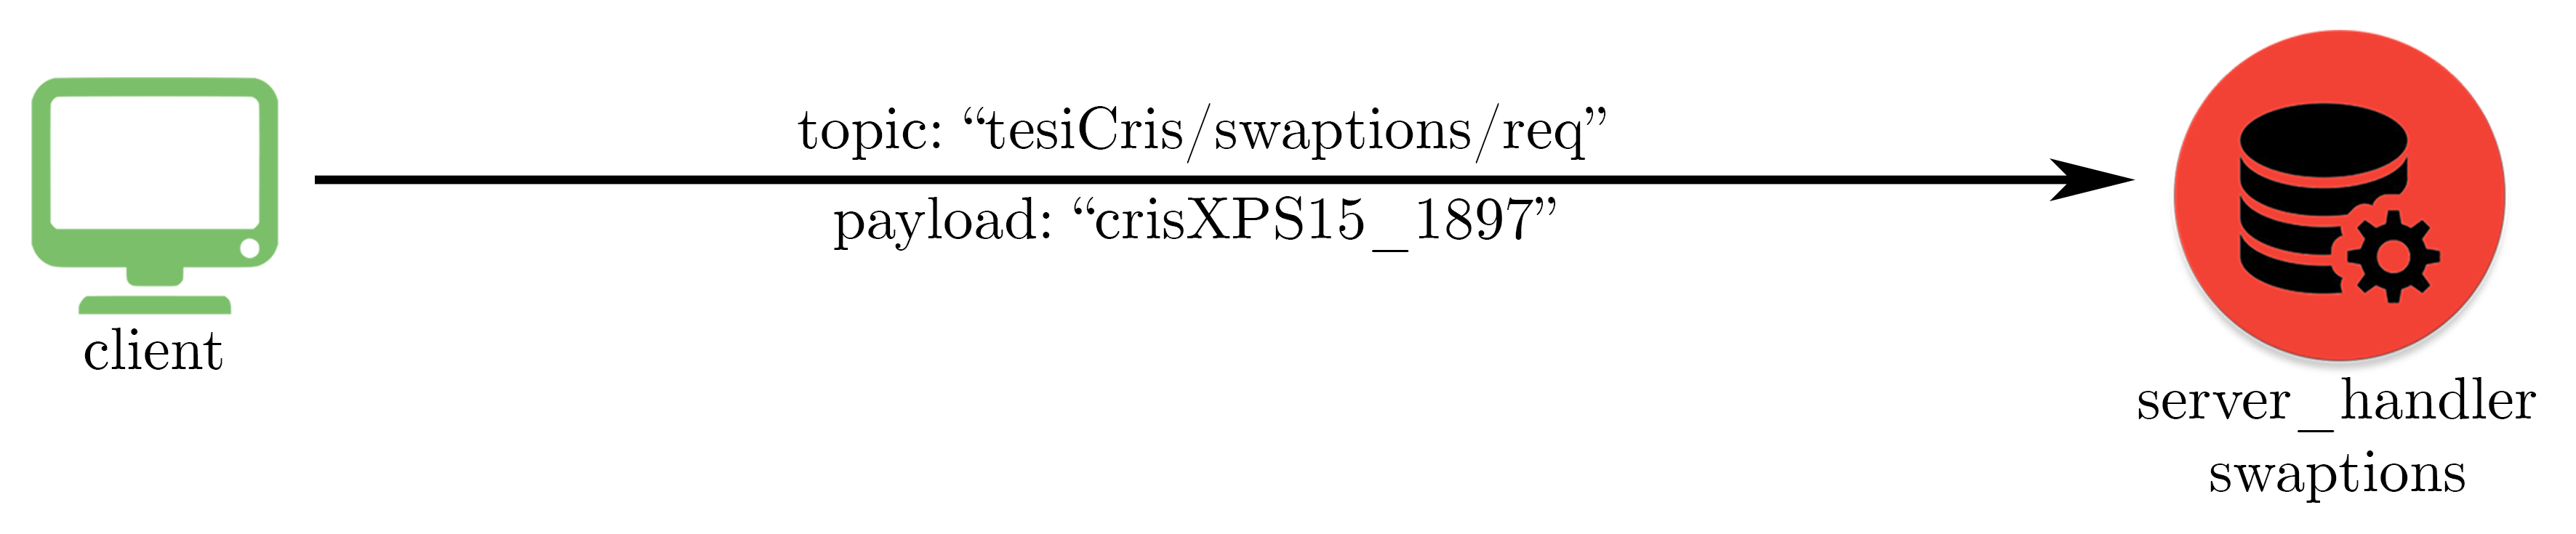
\includegraphics[width = \textwidth]{req}
    \caption{AgoraLocalAppHandler request example}

    \label{fig::localReq}
    
\end{figure}

This kind of publication is repeated until the node receives the predicted complete Operating Point list; AgoraRemoteAppHandler replies to these requests according to its internal state, that can be one of the following:

\begin{enumerate}

    \item \textit{unknown};

    \item \textit{receivingInfo};

    \item \textit{buildingDoE};

    \item \textit{DSE};

    \item \textit{buildingTheModel};

    \item \textit{autotuning}.

\end{enumerate}


\subsubsection{AgoraRemoteAppHandler internal state equal to \textit{unknown}}\label{req_info}

AgoraRemoteAppHandler doesn't know anything about the application it is managing, except its name; it asks to AgoraLocalAppHandler modules all available information, making a publication with payload "info" on topic "agora/\textit{[appName]}" (Figure \ref{fig::remotInfoReq}).

\begin{figure}[ht]

    \centering
    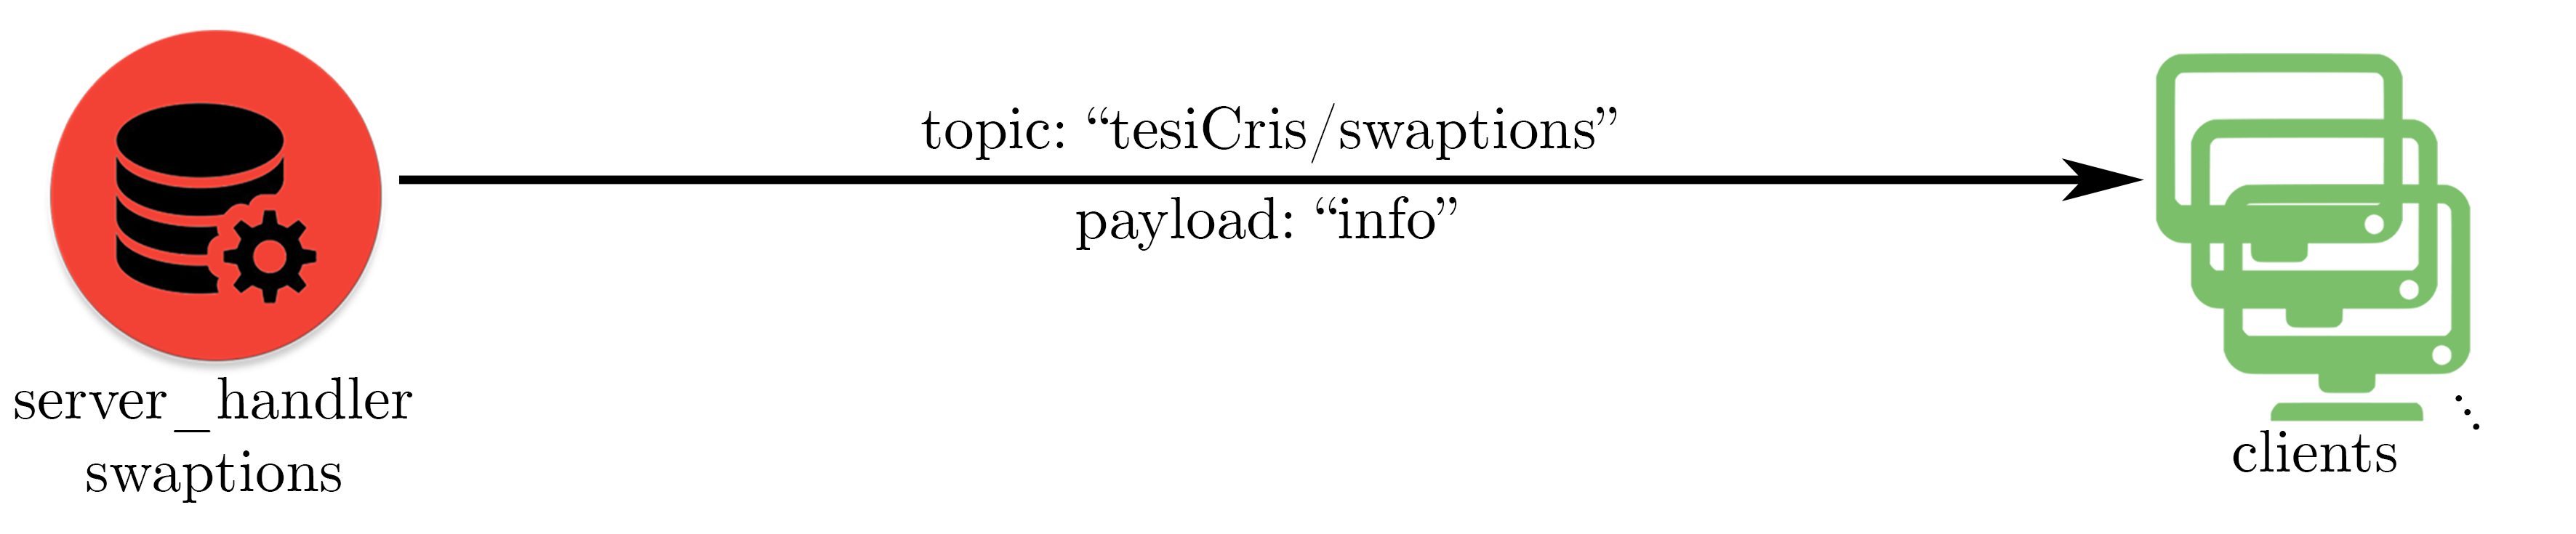
\includegraphics[width = \textwidth]{info_req}
    \caption{Application information request by \textit{AgoraRemoteAppHandler} example}

    \label{fig::remotInfoReq}
    
\end{figure}


\subsubsection{AgoraRemoteAppHandler internal state equal to \textit{receivingInfo}}

The AgoraRemoteAppHandler module is receiving application information, so in this case it discards all possible requests made by AgoraLocalAppHandler modules.


\subsubsection{AgoraRemoteAppHandler internal state equal to \textit{buildingDoE}}

AgoraRemoteAppHandler, according to the received Design of Experiments type (see \ref{client_info}), is building the set of configurations that are going to be distributed to AgoraLocalAppHandler modules during Design Space Exploration phase; also in this case it discards all possible AgoraLocalAppHandler module requests.


\subsubsection{AgoraRemoteAppHandler internal state equal to \textit{DSE}}\label{dse_conf}

The AgoraRemoteAppHandler module has computed DoE configurations, so it is driving Design Space Exploration phase; it picks up the first element on top of the available configuration list and it sends, in lexicographic order, the associated software knob values on topic "agora\slash{}\textit{[appName]}\slash{}\textit{[hostname]\_[PID]}\slash{}conf", relative to the AgoraLocalAppHandler module that made the request (Figure \ref{fig:conf}). The configuration just sent is reinserted at the end of the mentioned list.

\begin{figure}[ht]

    \centering
    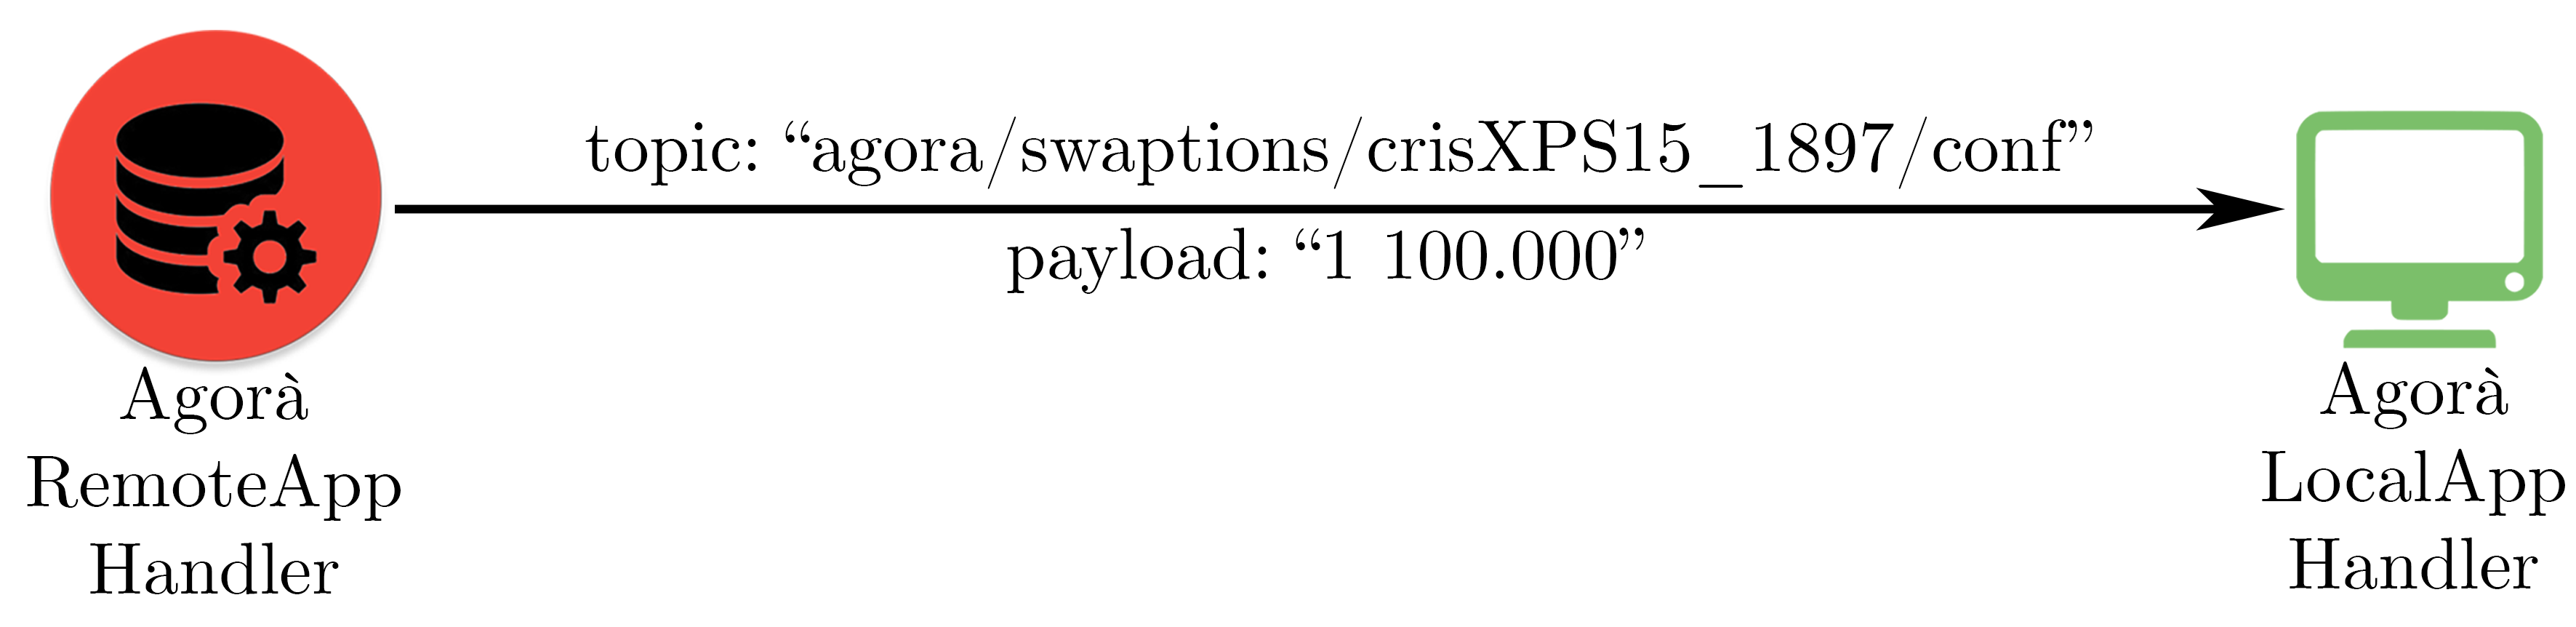
\includegraphics[width = \textwidth]{conf}
    \caption{Configuration dispatch by \textit{AgoraRemoteAppHandler} example}
    \label{fig:conf}
    
\end{figure}

As shown in Figure \ref{fig:conf}, AgoraLocalAppHandler receives a configuration with $num\_threads = 1$ and $num\_trials = 100.000$; next computation is going to be done with these parameter values.


\subsubsection{AgoraRemoteAppHandler internal state equal to \textit{building\-The\-Model}}\label{DoEModelSend}

AgoraRemoteAppHandler has gathered all needed OPs related to DoE configurations and it is computing complete Operating Point list through Machine Learning techniques; from gathered Operating Points, a partial model is built, assembling to every DoE configuration the mean of metric values, taken from the corresponding Operating Points; this partial model in sent to the Agora\-Local\-App\-Handler module that made the request: each obtained OP is published on topic "agora\slash{}\textit{[appName]}\slash{}\textit{[hostname]\_[PID]}\slash{}mod\-el" with format "\textit{[configuration] [metric values]}"; both configuration and metric values follow lexicographic order; finally, AgoraRemoteAppHandler makes a final publication on same topic with payload "DoEModelDone" (Figure \ref{fig:doe_model}).

\begin{figure}[hb]

    \centering
    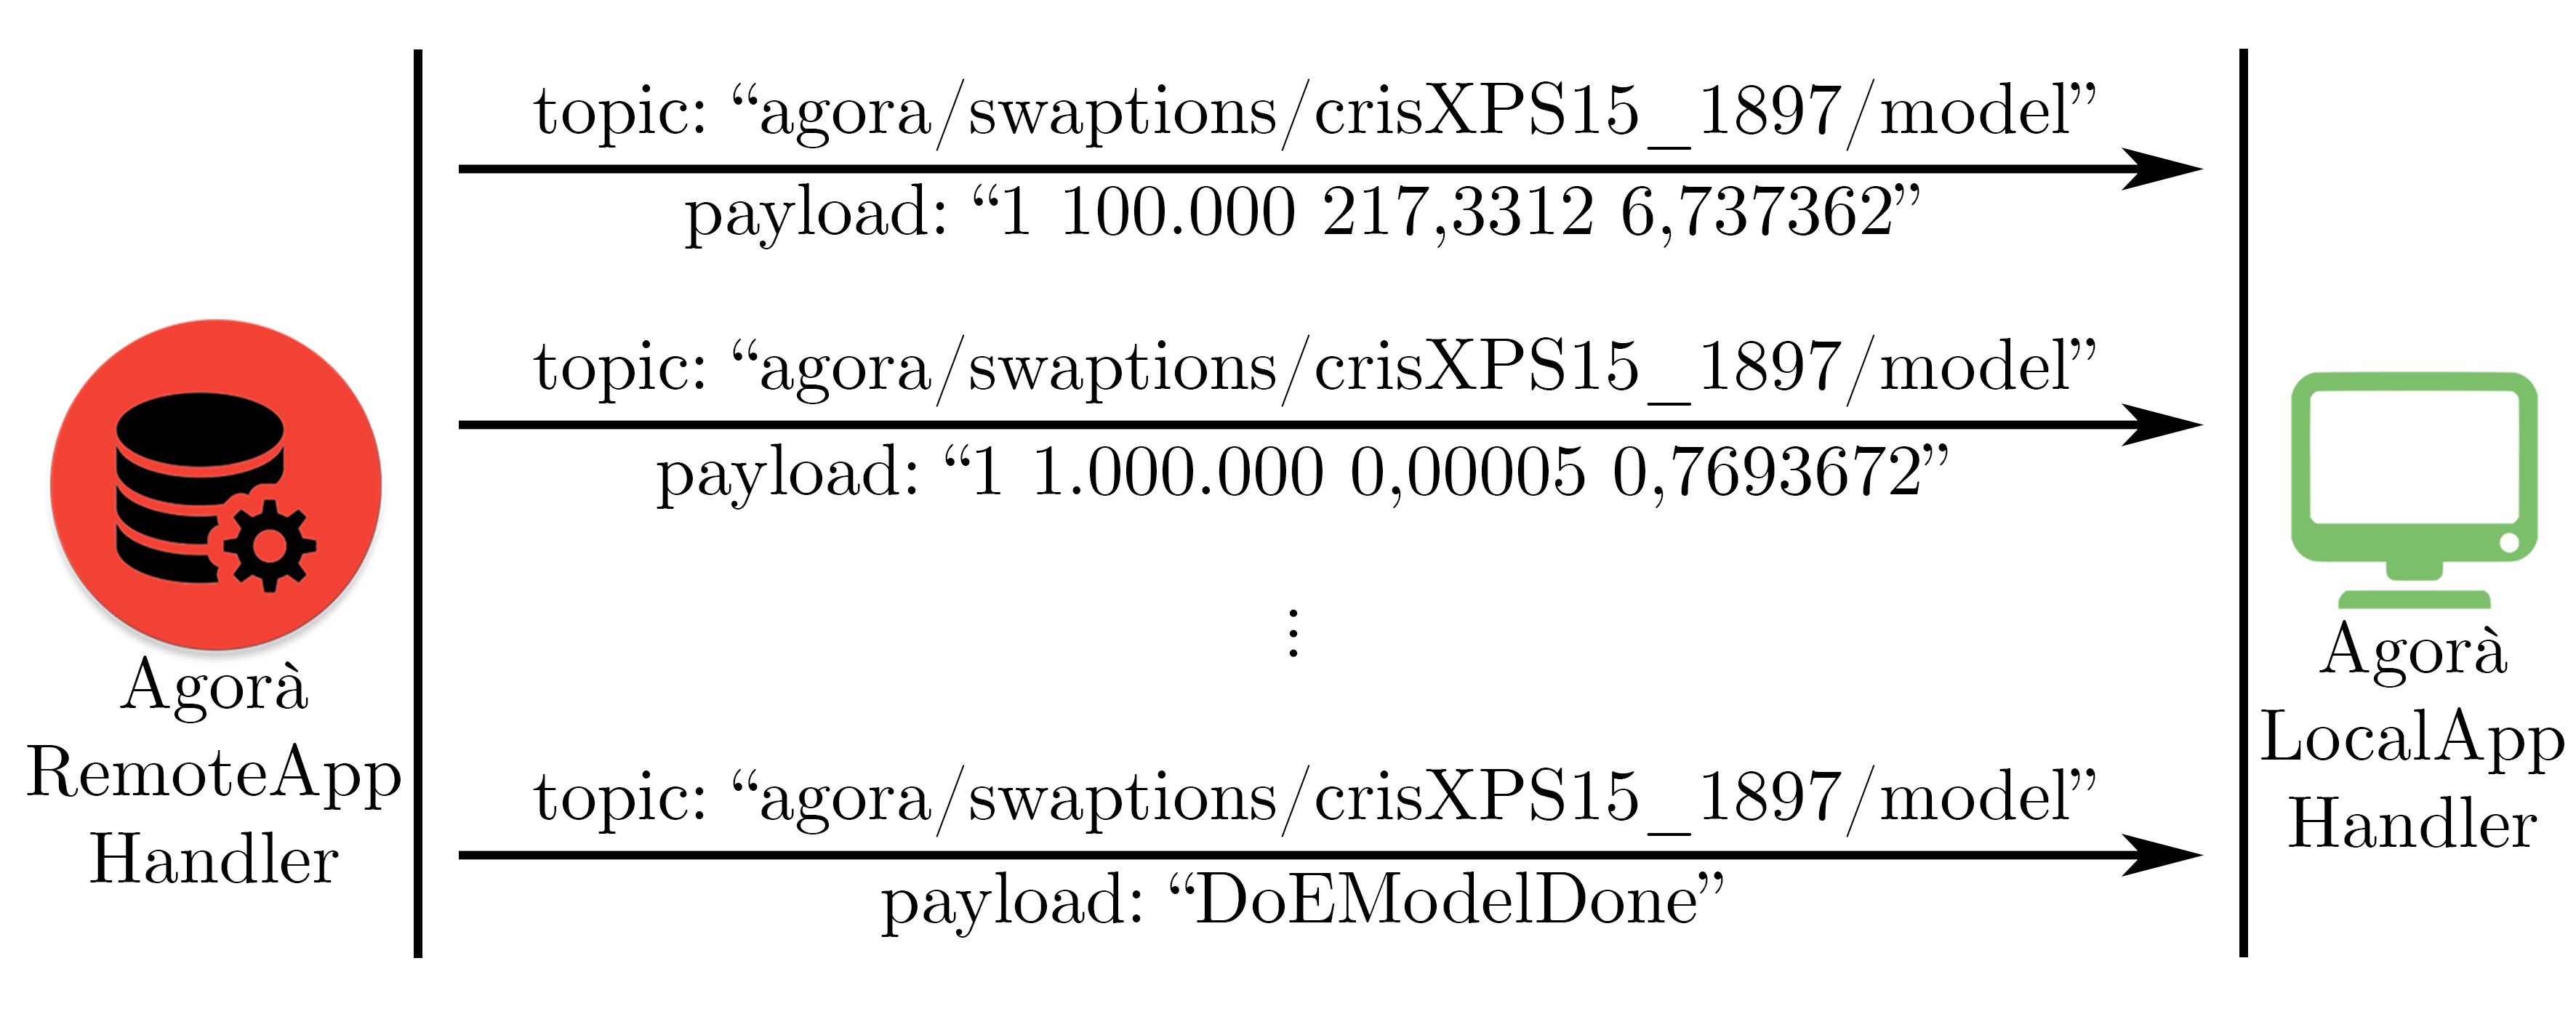
\includegraphics[width = \textwidth]{doe_model}
    \caption{Partial model dispatch by \textit{AgoraRemoteAppHandler} example}
    \label{fig:doe_model}
    
\end{figure}

Taking Figure \ref{fig:doe_model} as reference, the first sent OP has parameters\linebreak $num\_threads = 1$ and $num\_trials = 100.000$, with metrics $avg\_error = 217,3312$ and $avg\_throughput = 6,737362$; the AgoraLocalAppHandler module sets up mARGOt autotuner with this OP list, so the application is executed with the best Operating Point that fulfills current goals and requirements.


\subsubsection{AgoraRemoteAppHandler internal state equal to \textit{autotuning}}\label{modelSend}

The AgoraRemoteAppHandler module owns the complete OP list, obtained through the Generalized Linear Regression interface by A\-pach\-e Spark\textsuperscript{TM} MLlib library; similarly to the previous case (\ref{DoEModelSend}), every Operating Point is sent to AgoraLocalAppHandler on topic "agora\slash{}\textit{[app\-Name]}\slash{}\textit{[host\-name]\_[PID]}\slash{}model" with format "\textit{[configuration] [metrics values]}", respecting lexicographic order for both parameter and metric values; the final publication has payload "modelDone" (Figure \ref{fig:model}).

\begin{figure}[hb]

    \centering
    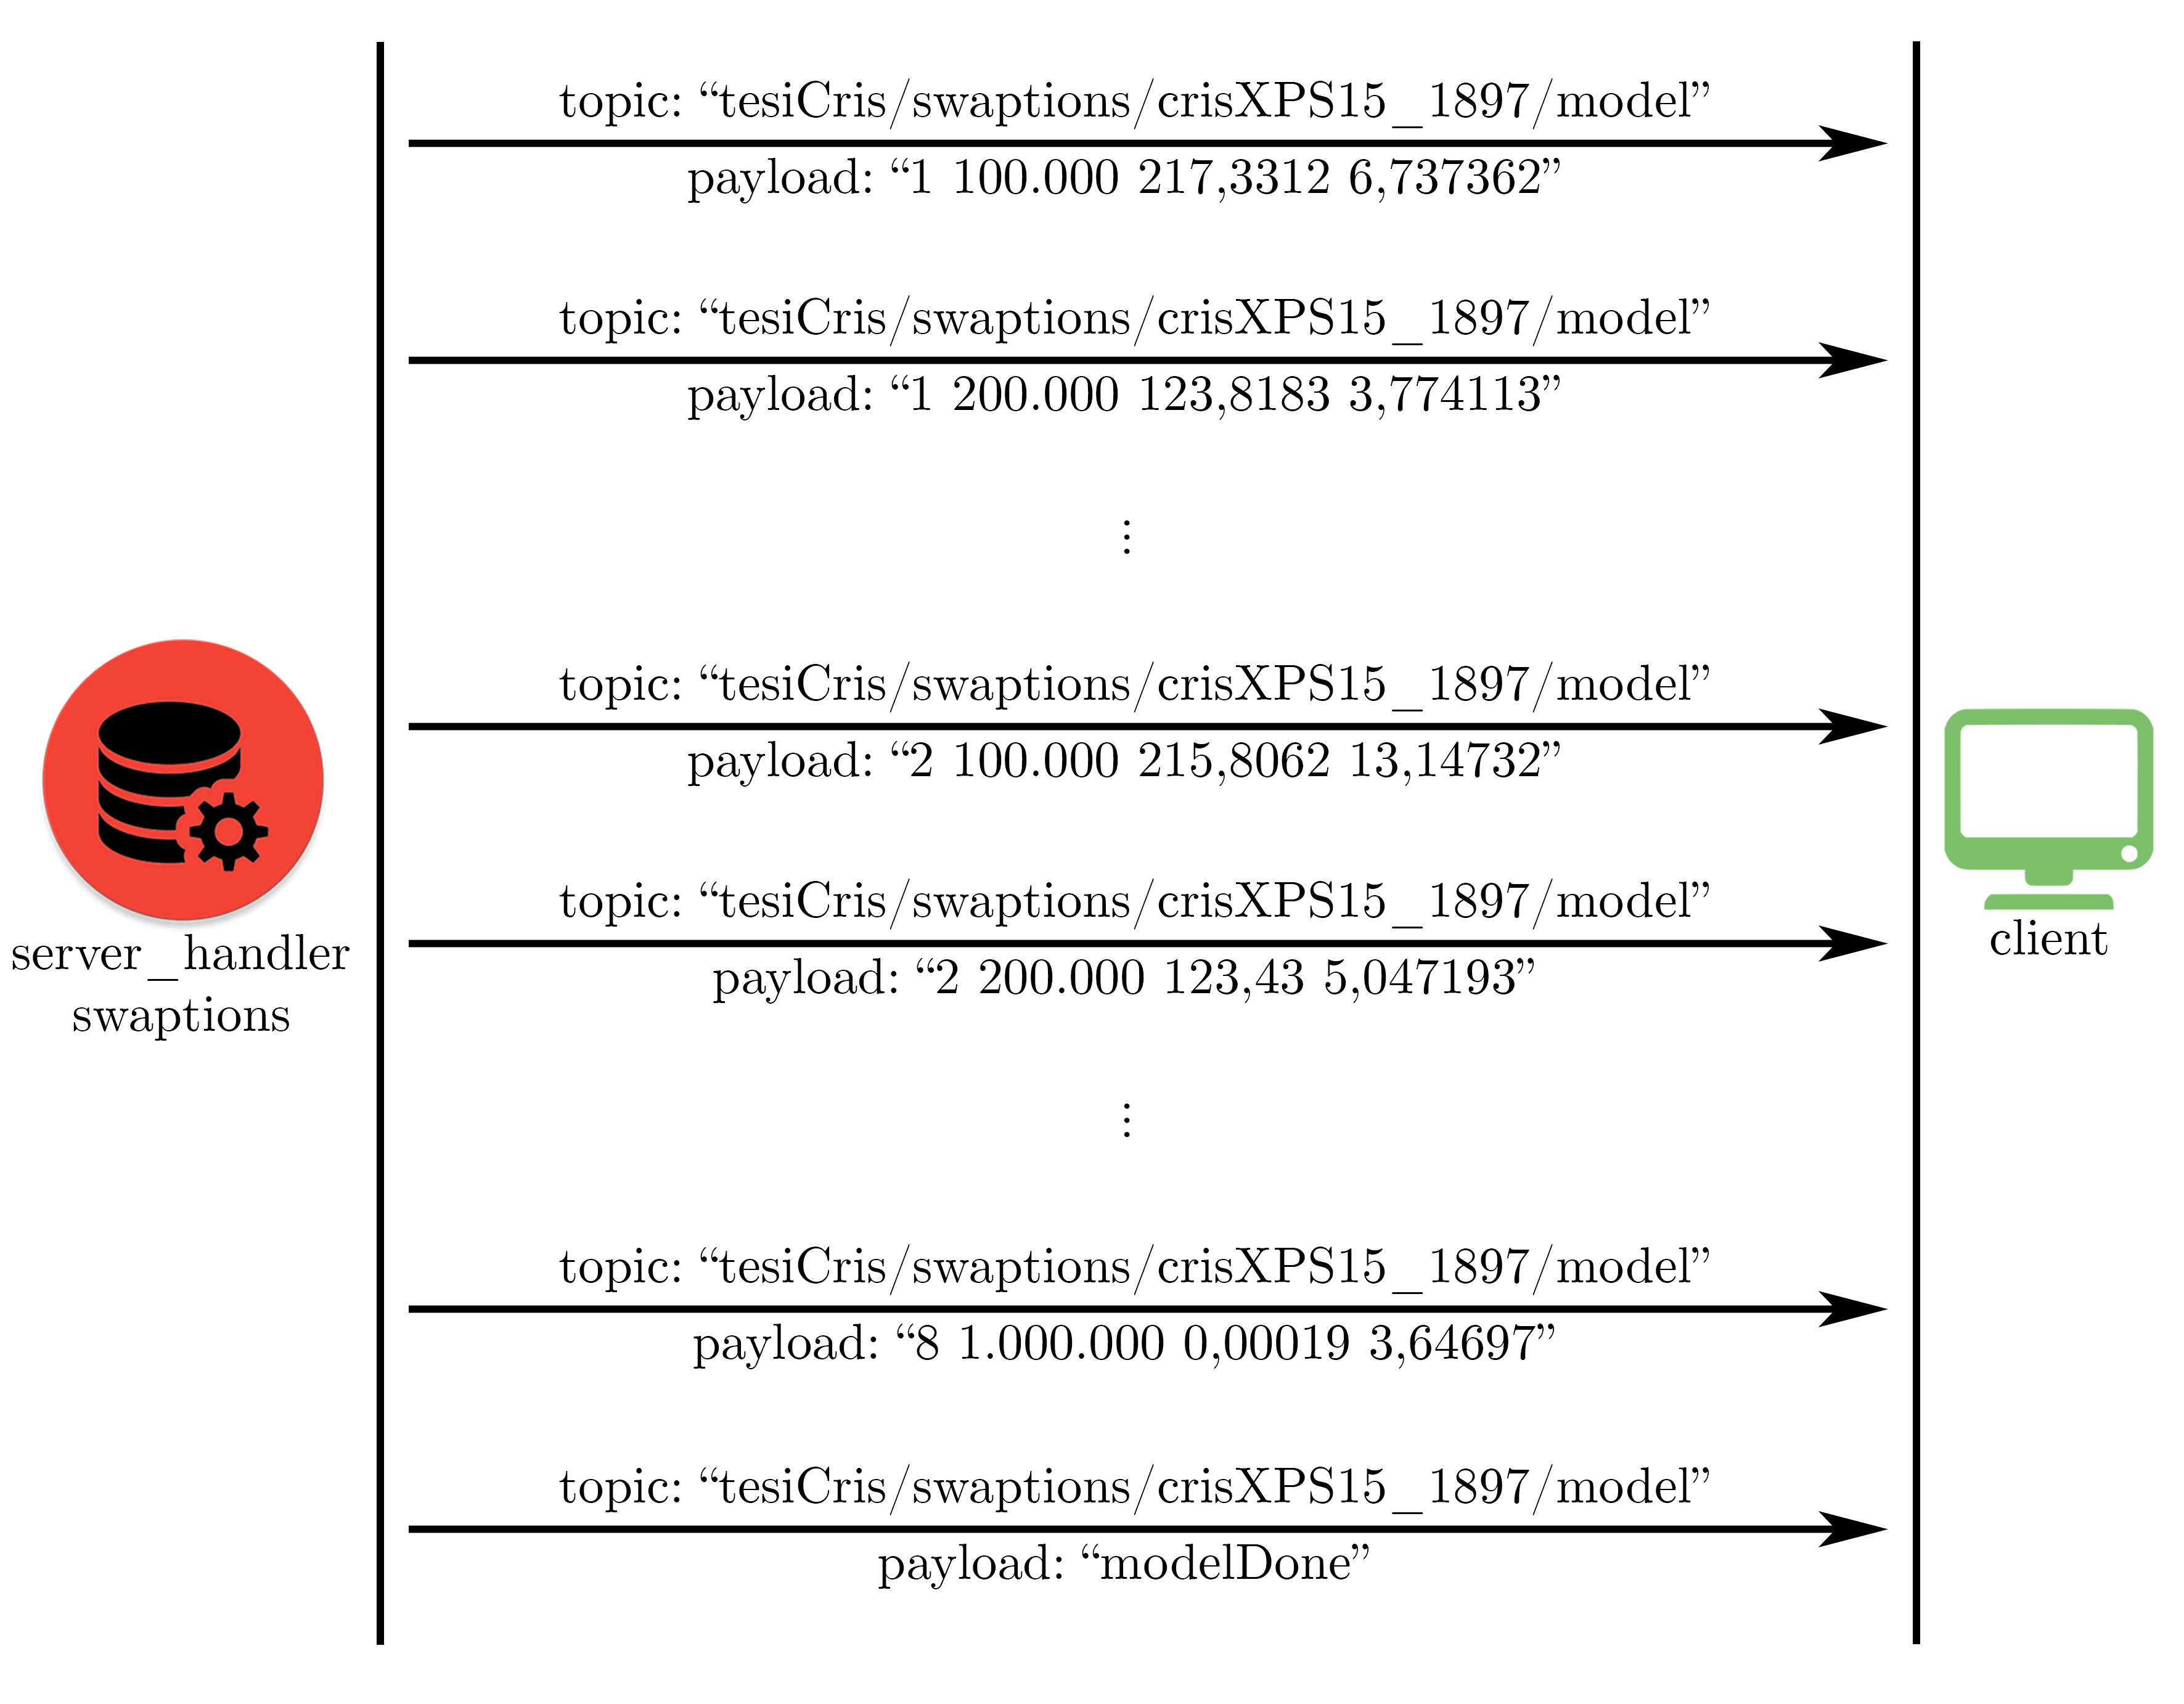
\includegraphics[width = \textwidth]{model}
    \caption{Complete model dispatch by \textit{AgoraRemoteAppHandler} example}
    \label{fig:model}
    
\end{figure}

In Swaptions application, parameter $num\_threads$ can assume 8 different values, while parameter $num\_trials$ 10 ones, so the complete model is composed by all the 80 OPs; after mARGOt autotuner has received all the predicted Operating Points, it can set up application knobs according to current objectives.

From this point on, AgoraLocalAppHandler stops making requests to the AgoraRemoteAppHandler module.





\subsection{Application information dispatch by AgoraLocalAppHandler}\label{client_info}

It has been shown that, if an AgoraRemoteAppHandler module receives a request from a node but its internal state is \textit{unknown}, it requests application information (see \ref{req_info}); AgoraRemoteAppHandler saves both the identifier of the first AgoraLocalAppHandler module that replies and all data it receives; other possible replies from other AgoraLocalAppHandler modules are discarded.

Mandatory information AgoraLocalAppHandler modules have to send is:

\begin{enumerate}

    \item metrics under examination: the keyword is \textit{metric}, followed by metric name; there is a publication for each metric; publications have to be in lexicographic order with respect to metric name;
    
    e.g. payload: "metric avg\_throughput"
    
    \item application parameters: the keyword is \textit{param}, followed by parameter name, the way in which it is transmitted and corresponding values; there is a publication for each parameter; also in this case, publications must follow lexicographic order with respect to parameter name; Agora makes available two ways to send values:
    
    \begin{enumerate}
    
        \item by list: the keyword is \textit{enum} and, in this case, all possible values are listed;
        
        \item by extreme values and step: the keyword is \textit{range} and, in this case, minimum value, maximum value and step are sent; AgoraRemoteAppHandler module, from this information, computes all possible parameter values.
    
    \end{enumerate}
    
    e.g. payload: "param num\_threads enum 1 2 3 4 5 6 7 8"
    
    e.g. payload: "param num\_trials range 100.000 1.000.000 100.000"

\end{enumerate}

There are some optional information that AgoraLocalAppHandler modules can send to the AgoraRemoteAppHandler:

\begin{enumerate}

    \item number of required repetitions for each Operating Point: the keyword is \textit{numReps}, followed by a number; this value represents the number of Operating Points that the AgoraRemoteAppHandler has to gather for each Design of Experiments configuration, during Design Space Exploration phase;
    
    e.g. payload: "numReps 5"
    
    \item Design of Experiments type: the keyword is \textit{DoE}, followed by the term that indicates the kind of Design of Experiments that has to be used; it can be:
    
    \begin{enumerate}
    
        \item \textit{fcccd}: it corresponds to the Face Centered Central Composite DoE with one Center Point;
        
        \item \textit{ff2l}: it corresponds to the 2-Level Full-Factorial DoE;
        
        \item \textit{pbd}: it corresponds to the Plackett-Burman DoE;
        
        \item \textit{lhd}: it corresponds to the Latin-Hypercube DoE; in this case, there is another optional information that can be sent to the AgoraRemoteAppHandler module: the number of configurations that have to be produced, with the word \textit{lhdSamples} followed by the desired value; if this information is not sent, the number of random configurations is equal to the number of application parameters;
        
        \item \textit{fcccdExtra}: it corresponds to the Face Centered Central Composite DoE with one Center Point plus the addition of other configurations through the Latin-Hypercube DoE; as in the previous case, the optional keyword \textit{lhdSamples} is used to express the number of extra configurations, otherwise they are equal to the number of parameters;
        
        \item \textit{fullFact}: it corresponds to the Full-Factorial DoE.
    
    \end{enumerate}
    
    We refer to Chapter \ref{doe} for Design of Experiments detailed information.
    
    e.g. payload: "DoE fcccdExtra"
    
    e.g. payload: "lhdSamples 6"
    
    \item Response Surface Modeling technique: the keyword is \textit{RSM}, followed by the term that indicates the Machine Learning technique that has to be used in order to predict application complete OP list; Agora implements two versions of the Apache Spark\textsuperscript{TM} Generalized Linear Regression, explained in detail in \ref{regrTransforms}:
    
    \begin{enumerate}
    
        \item the 1st version ("\textit{transformations by functions}"), that uses parameter values transformations, with associated word \textit{sparkGenLinRegrTransforms};
        
        \item the 2nd version ("\textit{polynomial combinations of degree 2}"), that uses parameter polynomial combinations of degree 2, with associated word \textit{sparkGenLinRegrPolyComb2}.
    
    \end{enumerate}
    
    e.g. payload: "RSM sparkGenLinRegrPolyComb2"
    
    \item parameter value transformations for the 1st implemented version of Apache Spark\textsuperscript{TM} Generalized Linear Regression RSM: the keyword is \textit{paramsTransforms}, followed by the involved metric name and the terms that indicate the kind of parameter transformations, the family distribution and the link function. Transformations must follow the same order of parameter information dispatch; they can be:
    
    \begin{enumerate}
    
        \item \textit{inv}: in this case, to the corresponding parameter values in the OPs, the inverse function is applied;
        
        \item \textit{ln}: in this case, to the corresponding parameter values in the OPs, the natural logarithmic function is applied;
        
        \item \textit{sqrt}: in this case, to the corresponding parameter values in the OPs, the square root function is applied;
        
        \item \textit{id}: in this case, the corresponding parameter values in the OPs are not transformed.
    
    \end{enumerate}
    
    Agora focuses on the prediction of continuous functions with normal distribution: corresponding family is the Gaussian one, indicated with word \textit{gaussian}. For Gaussian family, link function can be:
    
    \begin{enumerate}
    
        \item \textit{identity};
        
        \item \textit{log};
        
        \item \textit{inverse}.
    
    \end{enumerate}
    
    If this kind of information is available, it must exist for each metric of interest. We refer to Chapter \ref{glr} for more detailed information about family and link function.
    
    e.g. payload: "paramsTransforms avg\_error id sqrt gaussian log"
    
    \item number of application features: the keyword is \textit{numFeats}, followed by the corresponding number; in this case, a minimum number $n$ of feature value observations can be specified through the keyword \textit{minNumObsFeatValues}, followed by $n$: only those feature values that are observed at least $n$ times, during Design Space Exploration phase, contribute to the prediction of application complete OP list; if no feature value reaches $n$ observations, $n$ becomes the number of observations of the most observed feature value; if this last information is missing, $n = 1$.
    
    e.g. payload: "numFeats 1"
    
    e.g. payload: "minNumObsFeatValues 5"

\end{enumerate}

If not specified, default Design of Experiments type is Face Centered Central Composite DoE with one Center Point, default number of repetitions for each OP is 1, default number of program features is 0 and default RSM technique is the \textit{"polynomial combinations of degree 2"} version of the Apache Spark\textsuperscript{TM} Generalized Linear Regression. If the chosen RSM technique is the \textit{"transformations by functions"} GLR version but there is no information about parameter value transformations, Agora tries every possible combination in union with all possible link functions, choosing the best result according to Akaike Information Criterion measure and the mean of the sum of coefficient standard errors (see \ref{regrTransforms}).

All information is sent by AgoraLocalAppHandler modules on topic "agora\slash{}\textit{[appName]}\slash{}info\slash{}\textit{[hostname]\_[PID]}"; a final publication with message "done" specifies to the AgoraRemoteAppHandler that application information is finished. Taking Figure \ref{fig:info_send} as reference, the AgoraRemoteAppHandler pulls out, from topic, \textit{crisXPS15\_1897} and it saves this identifier as the AgoraLocalAppHandler that is sending program information; as we can see, \textit{Swaptions} application focuses on two metrics, $avg\_error$ and $avg\_throughput$; it has two parameters, $num\_threads$ and $num\_trials$; the former is sent with the complete list of values, while the latter is sent with the keyword \textit{range}, specifying its minimum value ($100.000$), its maximum one ($1.000.000$) and the step ($100.000$): the Agora\-Remote\-App\-Handler computes all values, that are therefore $100.000$, $200.000$, $300.000$, ..., $1.000.000$; the Design of Experiments that has to be used is the Face Centered DoE with one Center Point and the RSM technique is the 1st version of the Apache Spark\textsuperscript{TM} Generalized Linear Regression; parameter transformations are also specified so, e.g. for metric $avg\_error$, the first parameter ($num\_threads$) will not be transformed, while the second parameter ($num\_trials$) has to be transformed with the square root function, applying \textit{gaussian} as family distribution and \textit{log} as link function; it can be noticed that there is no information about the number of Operating Point repetitions to collect during DSE phase: in this case, default value is used (1 repetition for each OP); finally, there is no payload with keyword \textit{numFeats} either: \textit{Swaptions} does not have features.

The AgoraRemoteAppHandler module is now ready to compute Design of Experiments configurations; after that, it can start distributing them to nodes, driving the subsequent Design Space Exploration phase.

\begin{figure}[t]

    \centering
    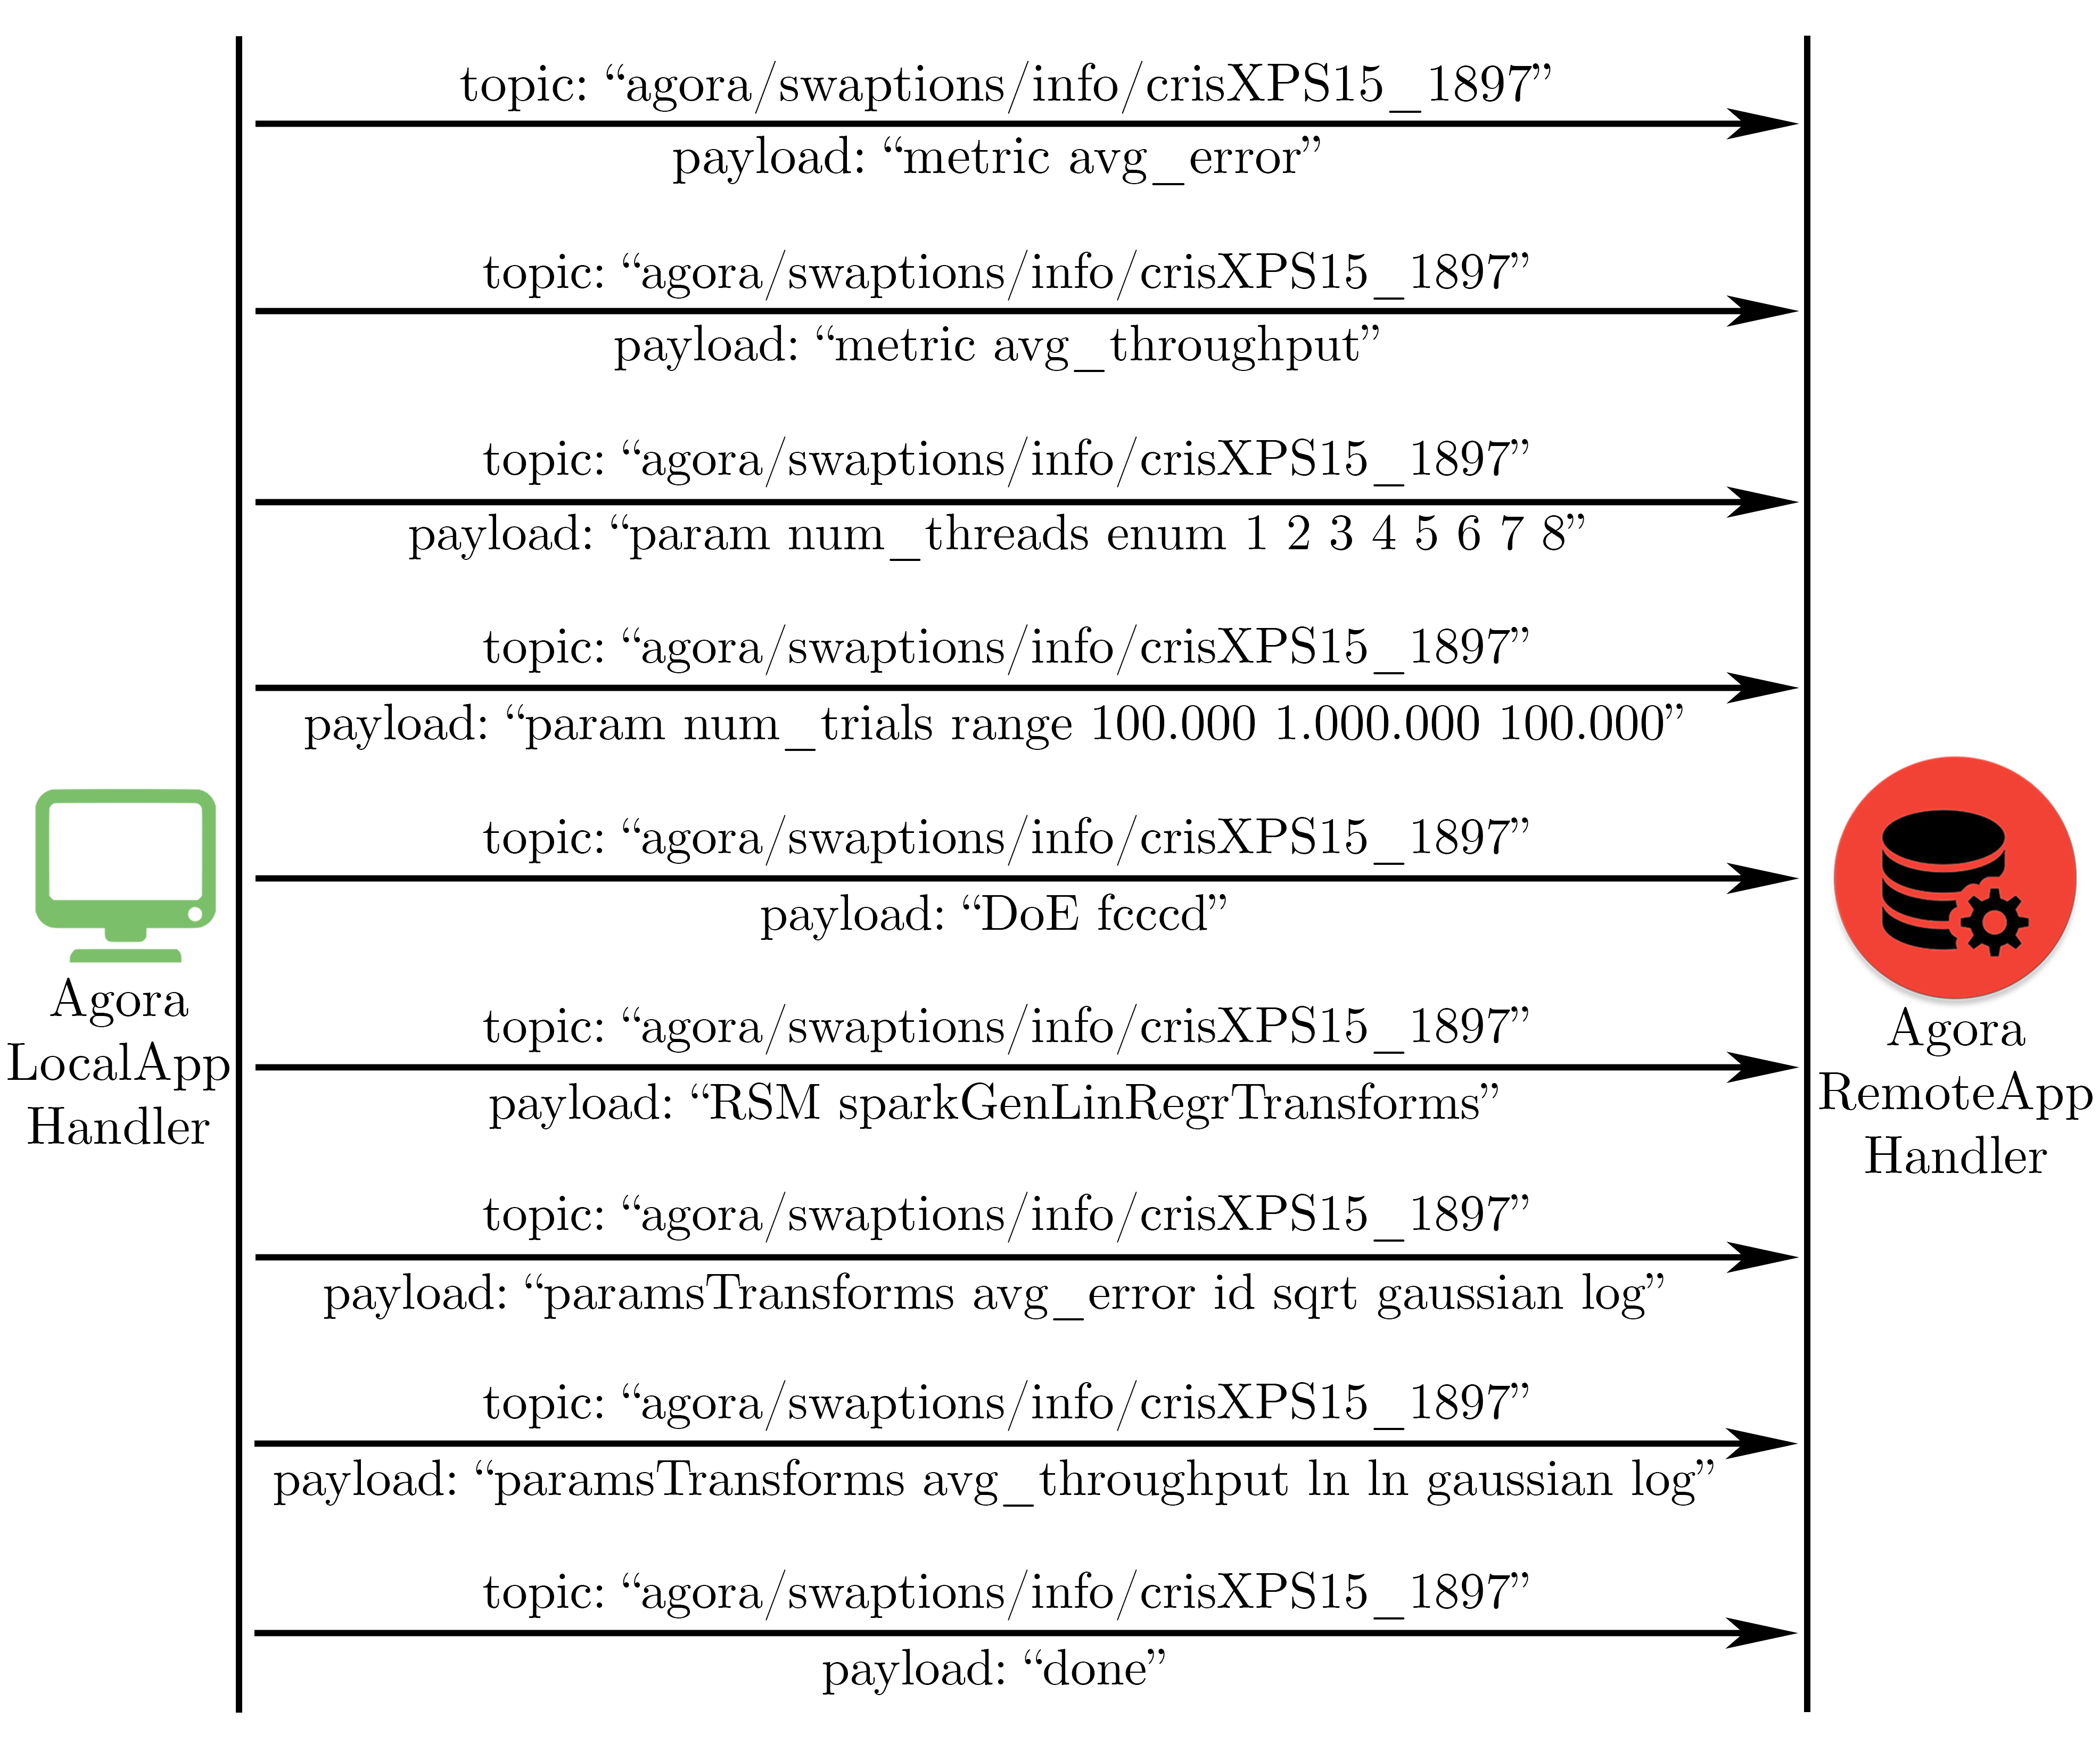
\includegraphics[width = \textwidth]{info_send}
    \caption{Application information dispatch by \textit{AgoraLocalAppHandler} module example}
    \label{fig:info_send}
    
\end{figure}





\subsection{Operating Point dispatch by AgoraLocalAppHandler module}\label{opSend}

During DSE, AgoraLocalAppHandler modules store configurations that receive from AgoraRemoteAppHandler (see \ref{dse_conf}); every time a configuration is sent, if the one in use differs from the new one, AgoraLocalAppHandler communicates to mARGOt autotuner new parameter values, therefore next program computation is executed with new parameter values.

When execution is finished, the AgoraLocalAppHandler module arranges the obtained Operating Point, composed by the set of parameter values and the observed metrics of interest; it publishes on topic "agora/\textit{[appName]}/OPs" a message in the form "\textit{[configuration]}:\textit{[metric values]}", in which both value lists have to follow lexicographic order with respect to parameter and metric name (Figure \ref{fig:op}). If there are application features, payload is in the form "\textit{[configuration]}:\textit{[ob\-served feature values]}:\textit{[metric values]}".

\begin{figure}[htb]

    \centering
    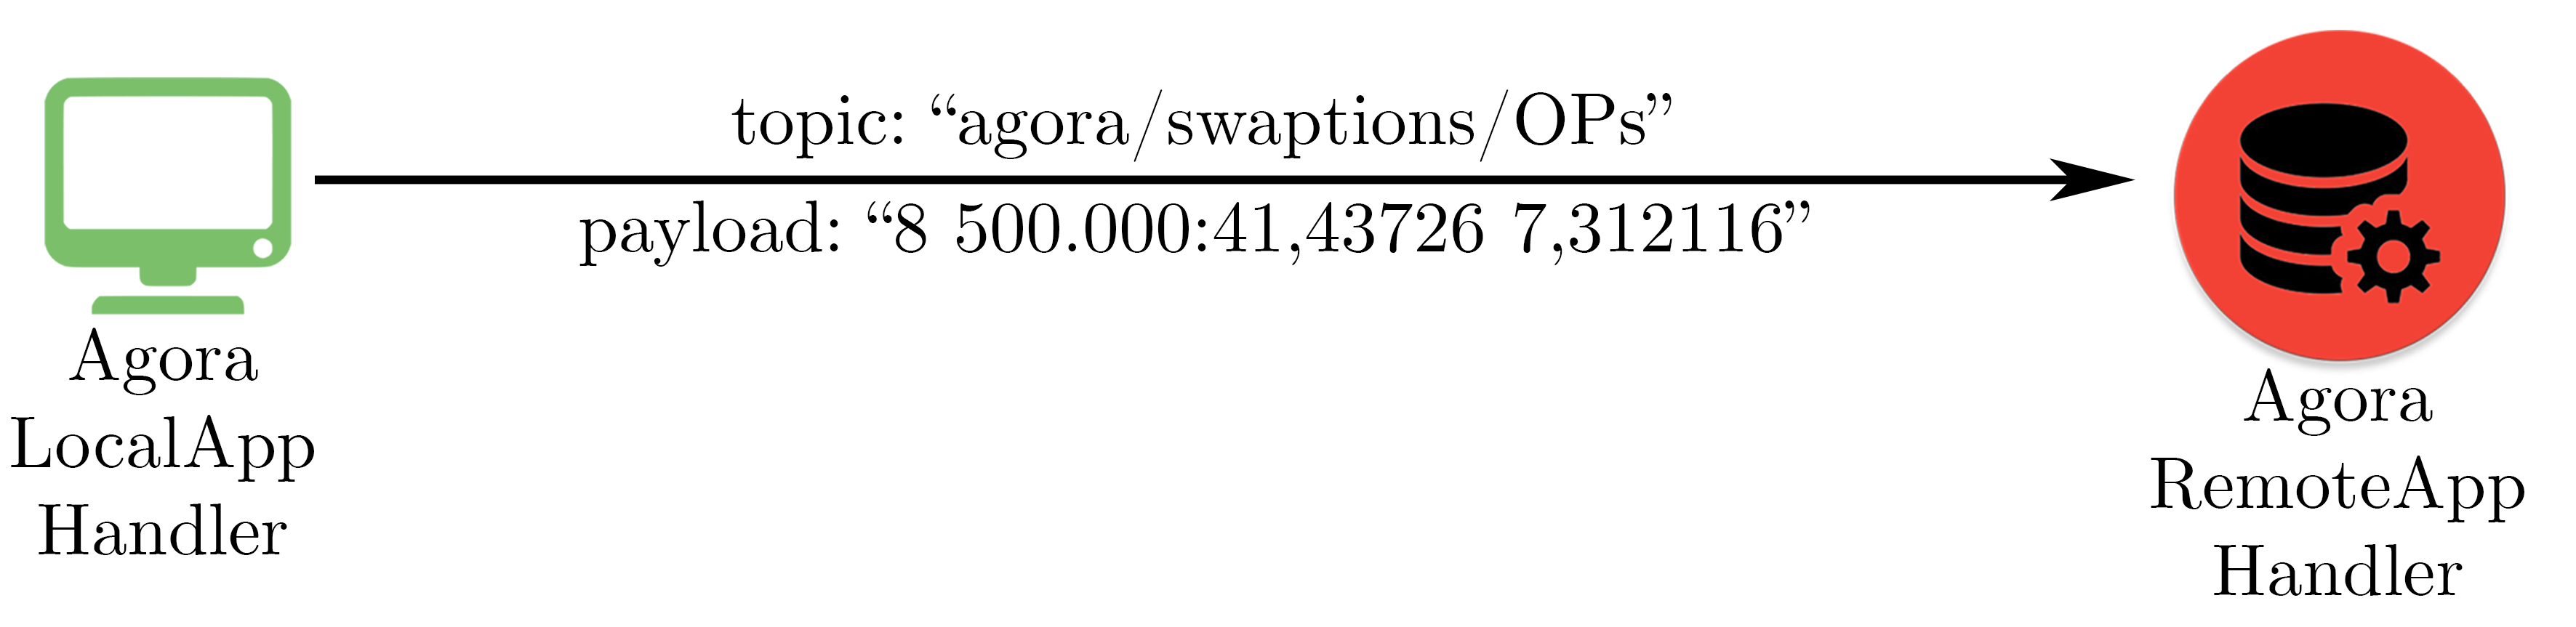
\includegraphics[width = \textwidth]{op}
    \caption{Operating Point dispatch by \textit{AgoraLocalAppHandler} module example}
    \label{fig:op}
    
\end{figure}

Taking Figure \ref{fig:op} as reference, \textit{Swaptions} has been just executed with\linebreak $num\_threads = 8$ and $num\_trials = 500.000$; monitored metric values are $avg\_error = 41,43726$ and $avg\_throughput = 7,312116$.

When AgoraRemoteAppHandler receives an Operating Point, it decrements the corresponding number of needed OP repetitions: if the updated value is equal to zero, it means that there is no need of other related OPs, so the corresponding configuration is moved from the set of available ones to the set of accomplished ones.

Model prediction just starts when last needed Operating Point repetition related to last available configuration is received from a node.





\subsection{AgoraLocalAppHandler module disconnection}\label{client_disc}

If an AgoraLocalAppHandler module disconnects for some reason, related Agora\-Remote\-App\-Handler receives a message on topic "agora\slash{}\textit{[appName]}\slash{}dis\-con\-nec\-tion" with payload "\textit{[hostname]\_[PID]}", relative to disconnected AgoraLocalAppHandler; the AgoraRemote\-App\-Handler module removes node identifier from the list of machines it is managing (Figure \ref{fig::locDisc}).

\begin{figure}[ht]

    \centering
    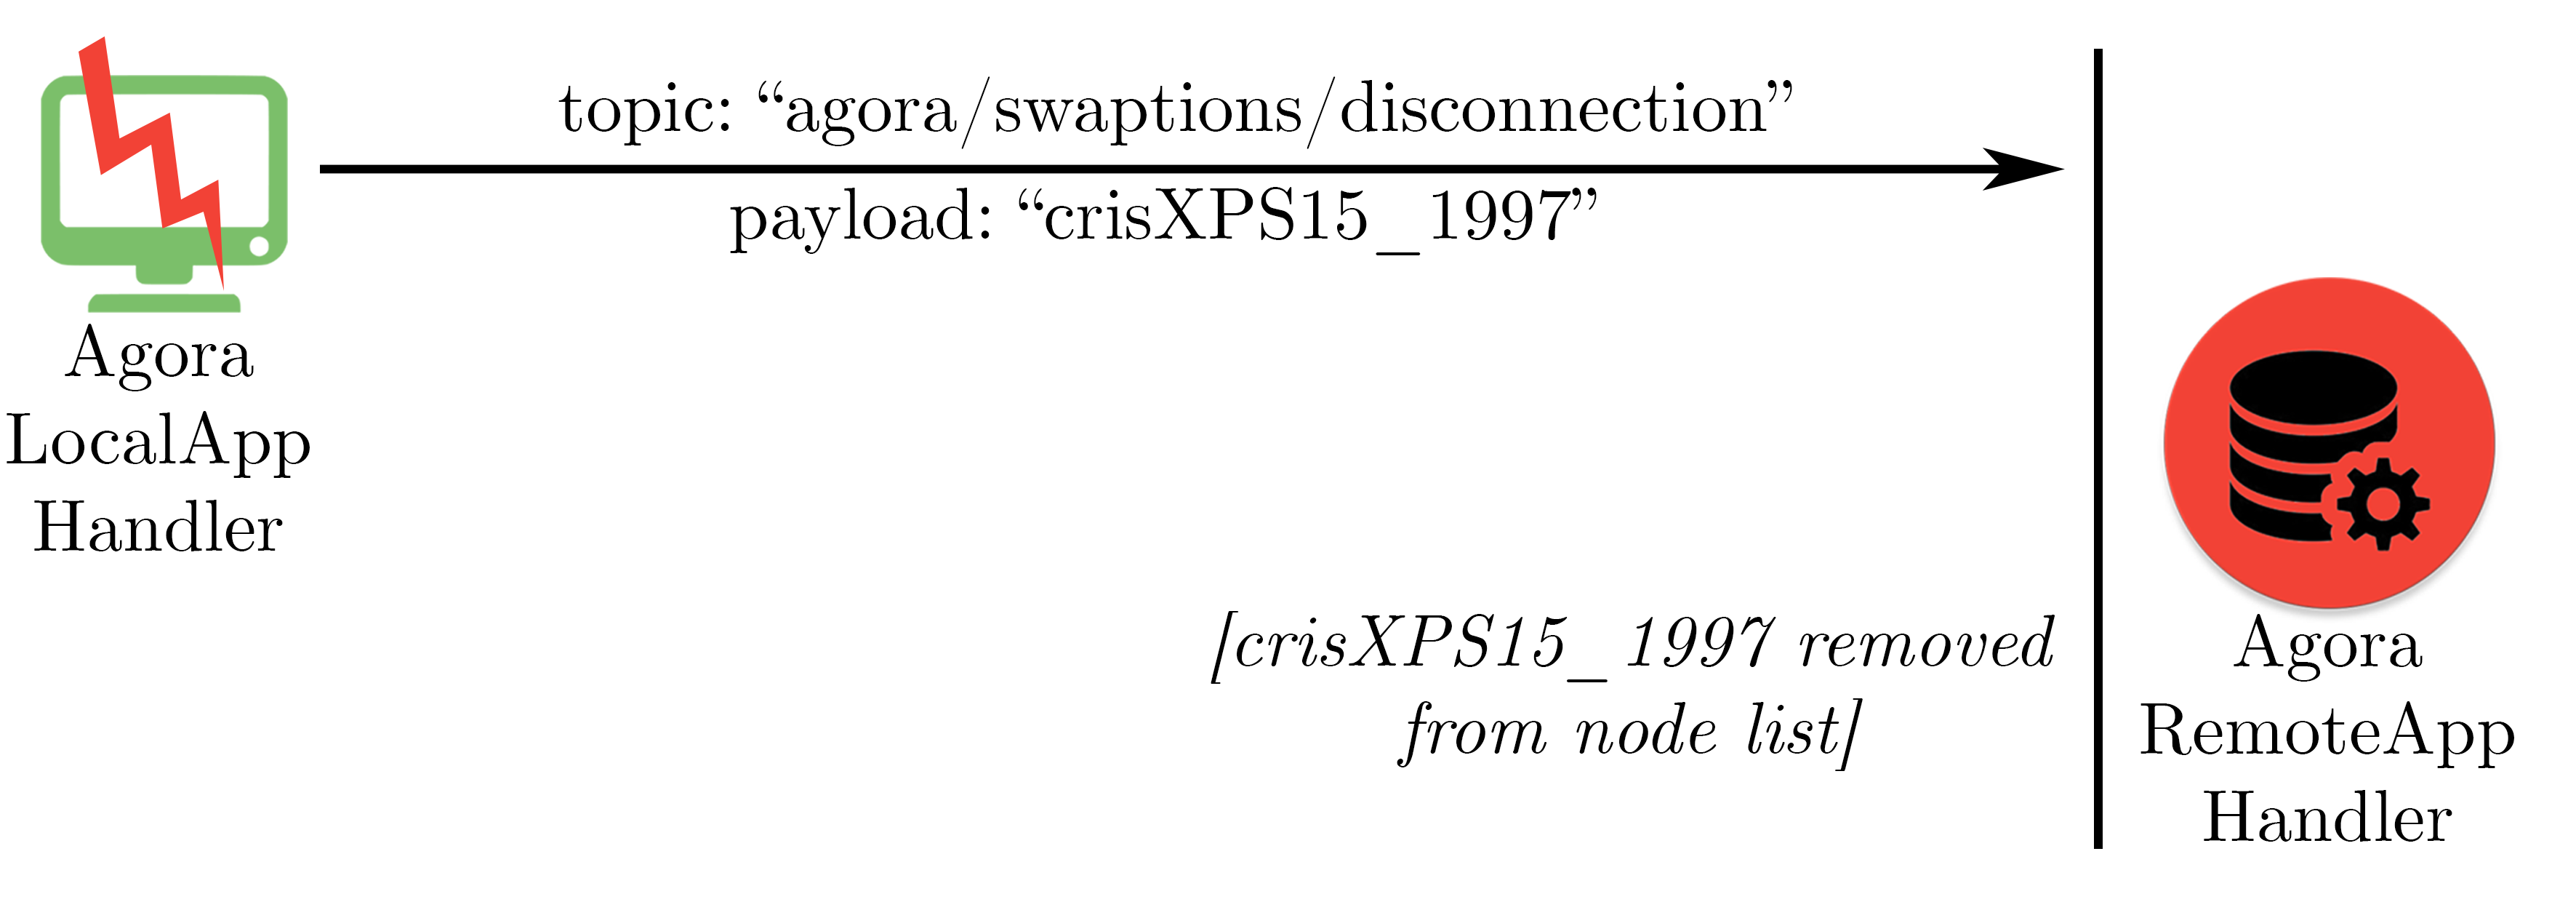
\includegraphics[width = \textwidth]{client_disc}
    \caption{AgoraLocalAppHandler module disconnection example}

    \label{fig::locDisc}
    
\end{figure}

Particular attention has to be taken if the disconnected AgoraLocalAppHandler module is the one that, at the beginning, is sending application information (see \ref{client_info}): in this case, AgoraRemoteAppHandler has to remove disconnected machine, it has to reset partial data (received up to that moment) and it asks again all available application information to remaining connected Agora\-Local\-App\-Handler modules (Figure \ref{fig::locInfoDisc}).

\begin{figure}[hb]

    \centering
    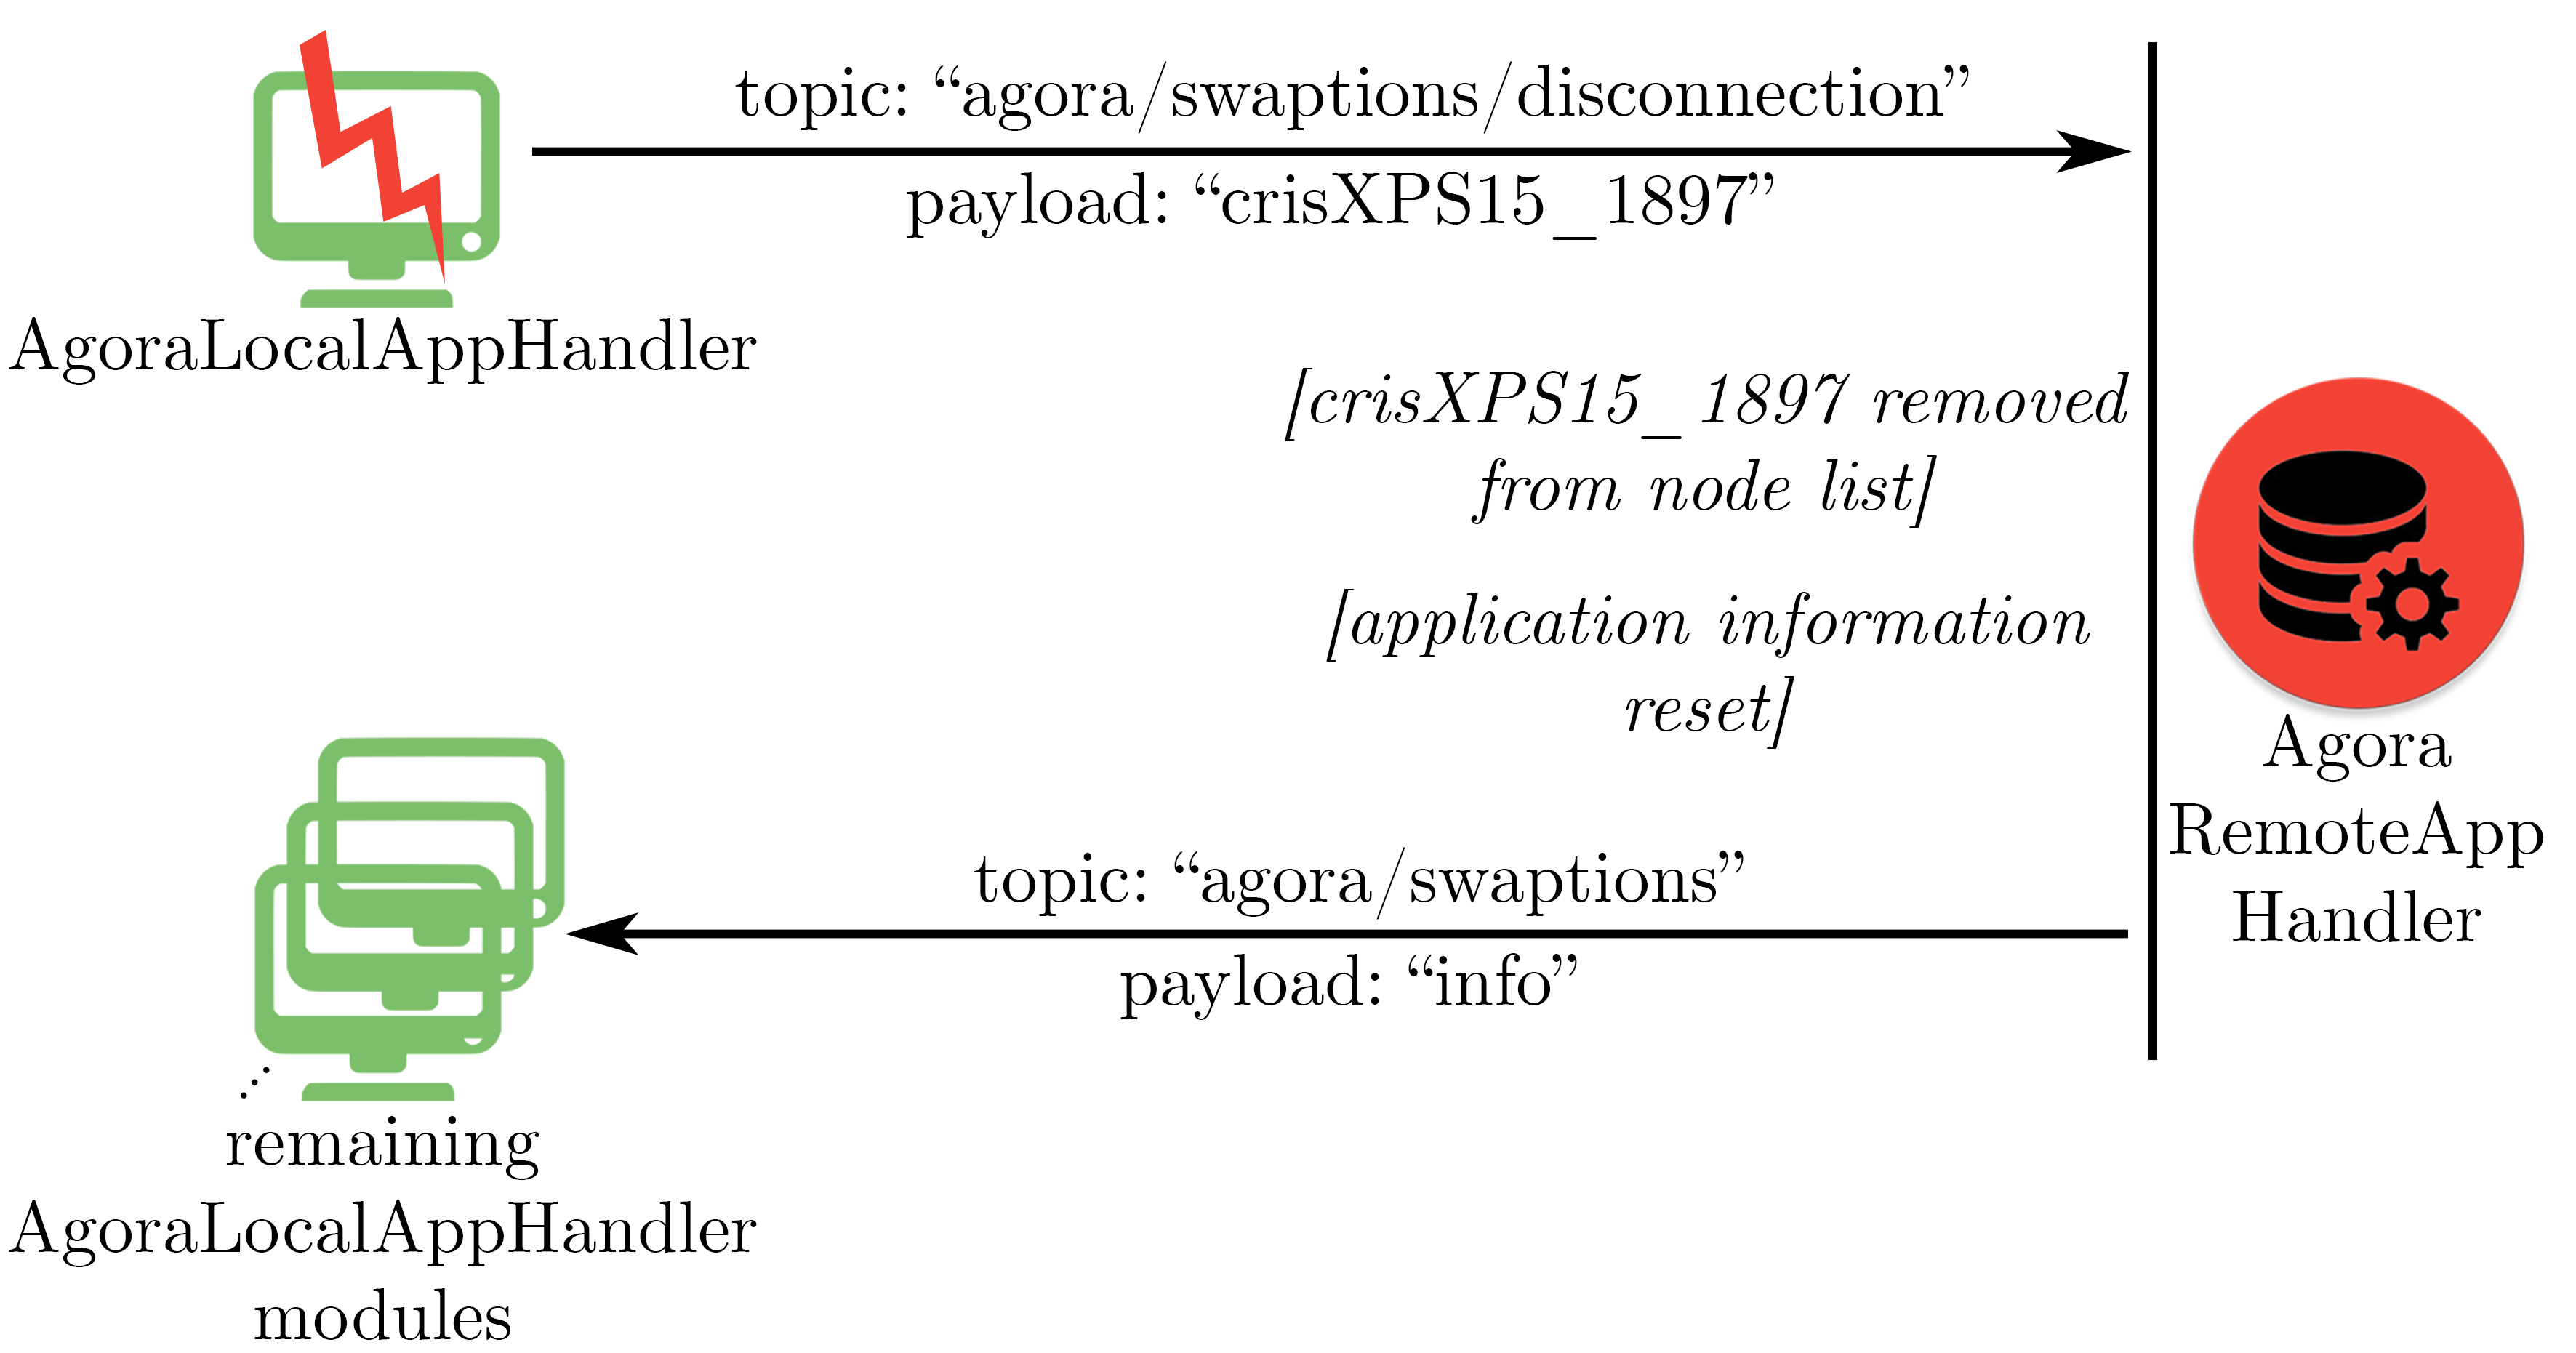
\includegraphics[width = \textwidth]{infoclient_disc}
    \caption{Disconnection of \textit{AgoraLocalAppHandler} module that was sending application information example}

    \label{fig::locInfoDisc}
    
\end{figure}





\subsection{AgoraRemoteAppHandler module disconnection}\label{handler_disc}

If the AgoraRemoteAppHandler module disconnects, related AgoraLocalAppHandler modules receive a message on topic "agora\slash{}\textit{[appName]}" with payload "disconnection" (Figure \ref{fig::remDisc}).

\begin{figure}[htb]

    \centering
    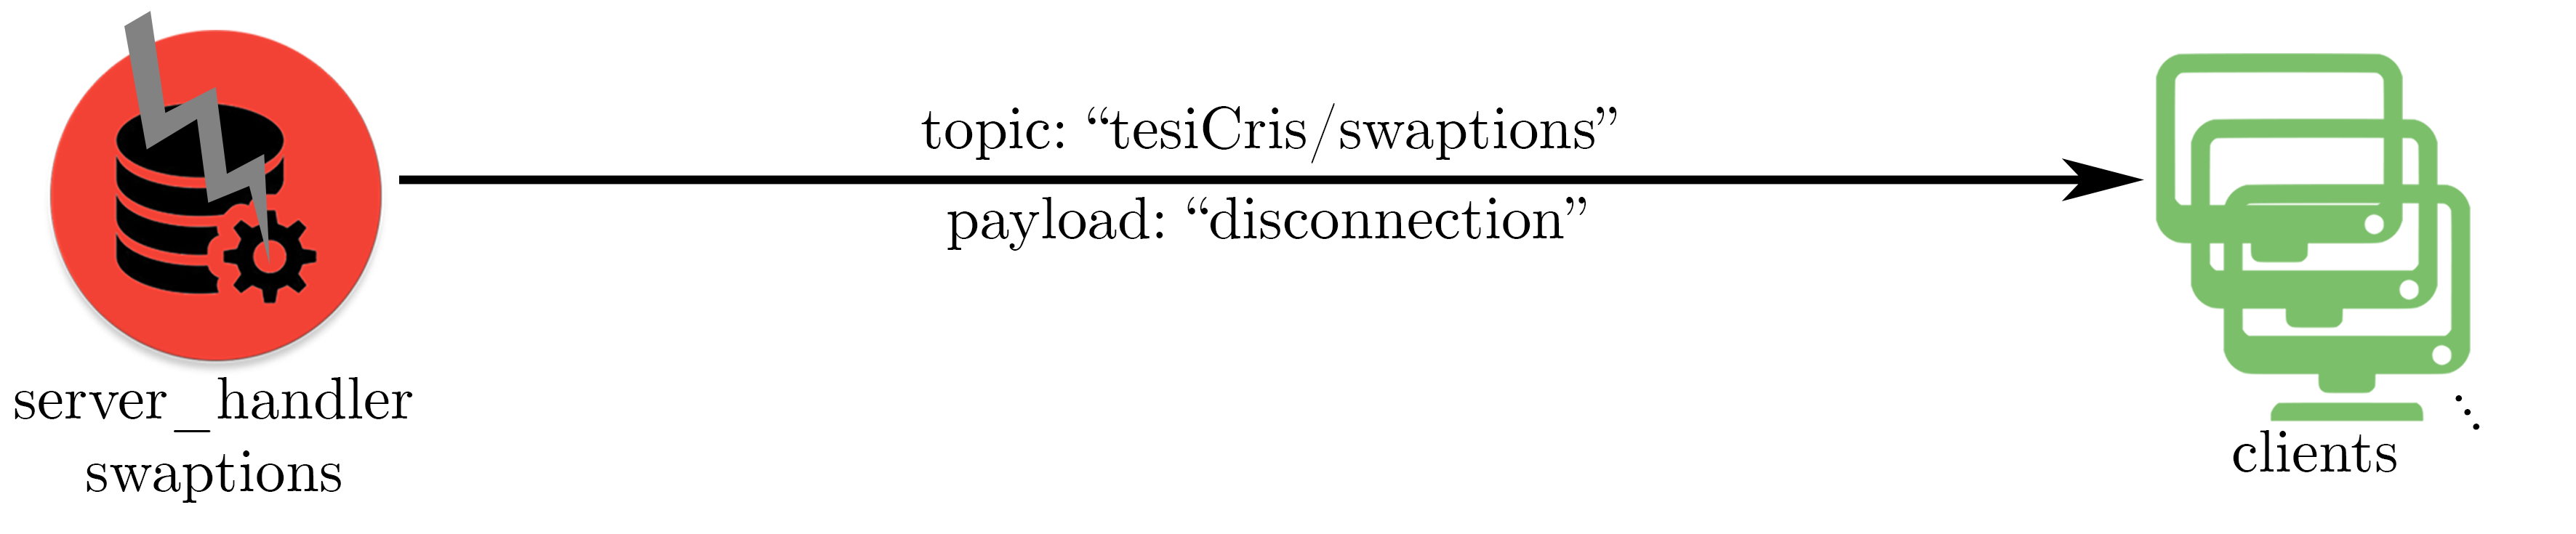
\includegraphics[width = \textwidth]{server_disc}
    \caption{AgoraRemoteAppHandler module disconnection example}

    \label{fig::remDisc}
    
\end{figure}

Each AgoraLocalAppHandler reacts to this event according to its internal state, that can be:

\begin{enumerate}

    \item \textit{defaultStatus};
    
    \item \textit{DSE};
    
    \item \textit{DoEModel};
    
    \item \textit{autotuning}.

\end{enumerate}


\subsubsection{AgoraLocalAppHandler internal state equal to \textit{defaultStatus}}

When a node starts running a program, the autotuner sets up application parameter values with a predetermined default configuration; if any Design Space Exploration phase has not been started yet, AgoraRemoteAppHandler disconnection does not affect application behavior.


\subsubsection{AgoraLocalAppHandler internal state equal to \textit{DSE}}

The AgoraRemoteAppHandler module is driving Design Space Exploration phase, sending configurations to AgoraLocalAppHandler modules; in this case, default configuration is restored and the application is executed with corresponding parameter values (Figure \ref{fig::remDiscDSE}).

\begin{figure}[htb]

    \centering
    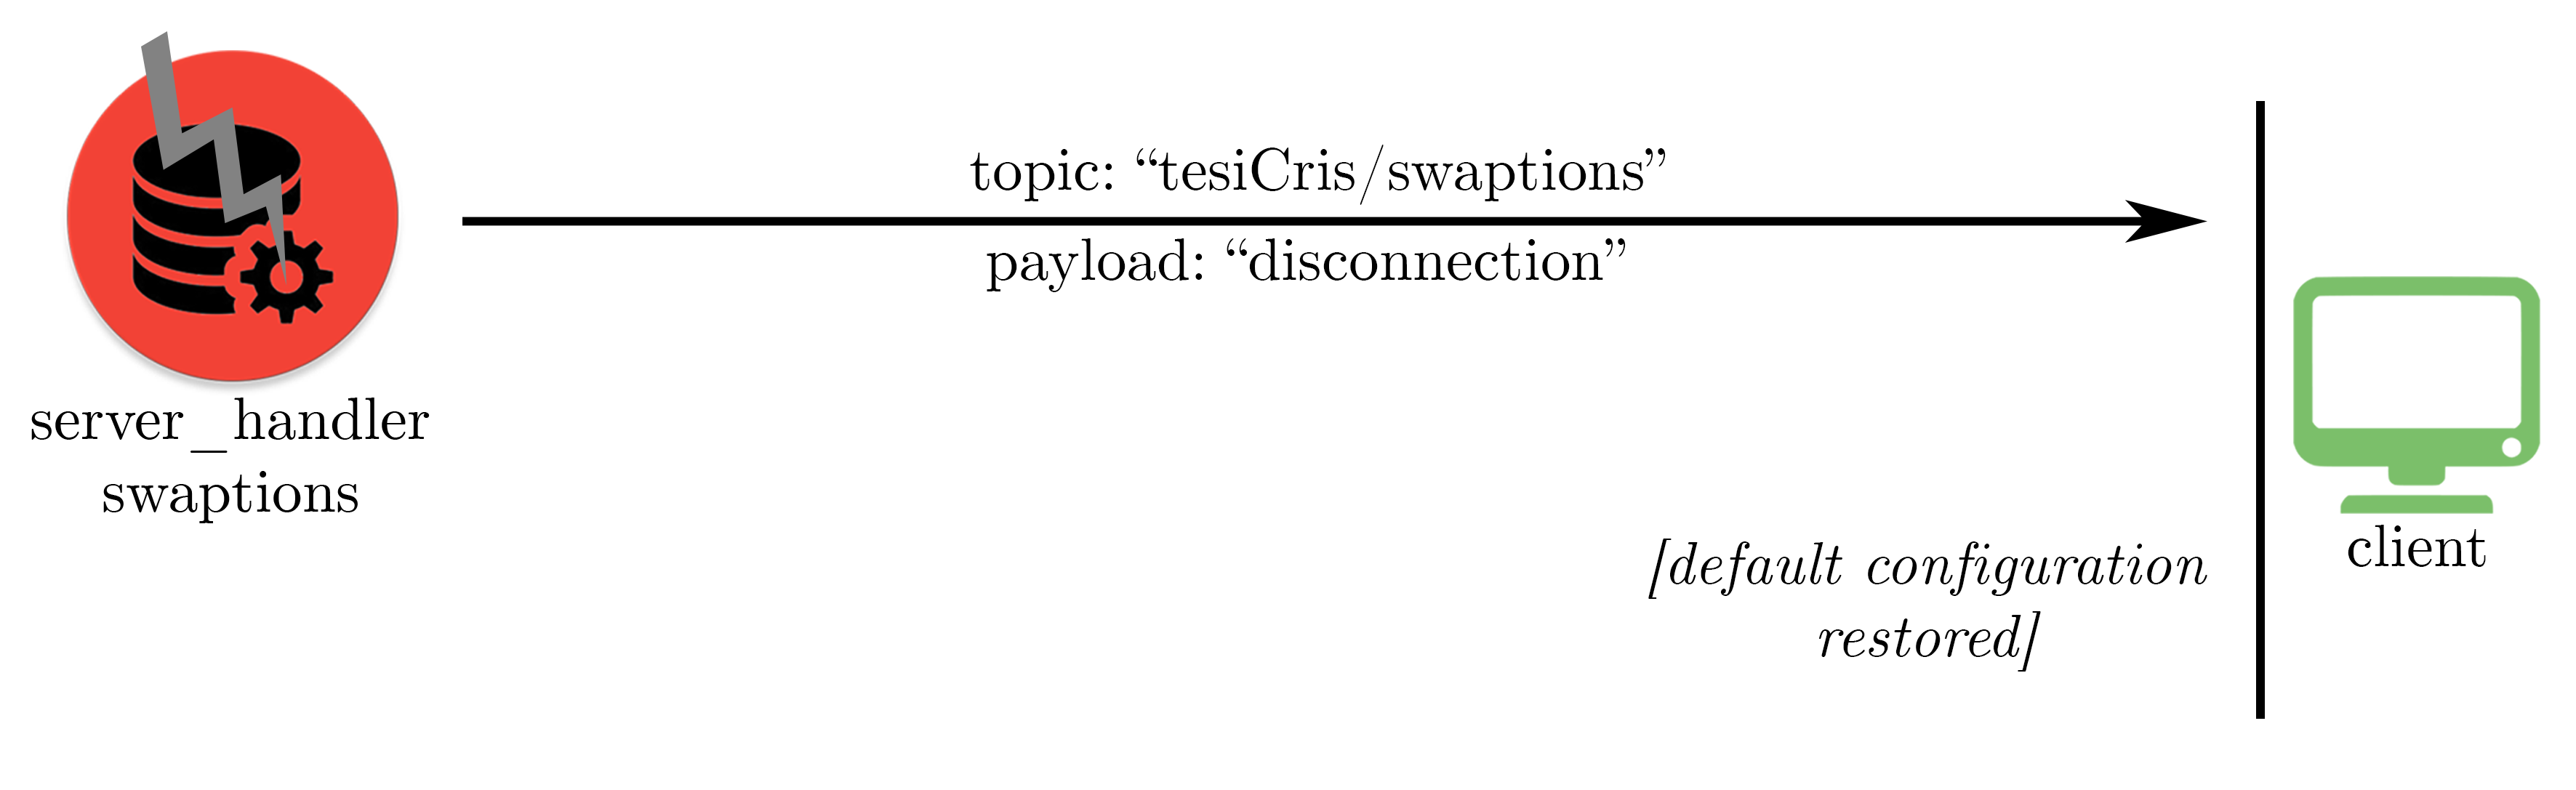
\includegraphics[width = \textwidth]{DSEinternal}
    \caption{AgoraRemoteAppHandler module disconnection with A\-go\-ra\-Local\-App\-Handler internal state equal to \textit{DSE} example}

    \label{fig::remDiscDSE}
    
\end{figure}


\subsubsection{AgoraLocalAppHandler internal state equal to \textit{DoEModel}}

AgoraLocalAppHandler has received a partial OP list, related to Design of Experiments configurations (see \ref{DoEModelSend}); in this case, available OP list is not deleted, therefore the autotuner continues to work with this information.


\subsubsection{AgoraLocalAppHandler internal state equal to \textit{autotuning}}

The AgoraLocalAppHandler module has already received predicted complete OP list from AgoraRemoteAppHandler, therefore nothing changes.





\section{AgoraLocalAppHandler module integration}

\begin{figure}[htb]

    \centering
    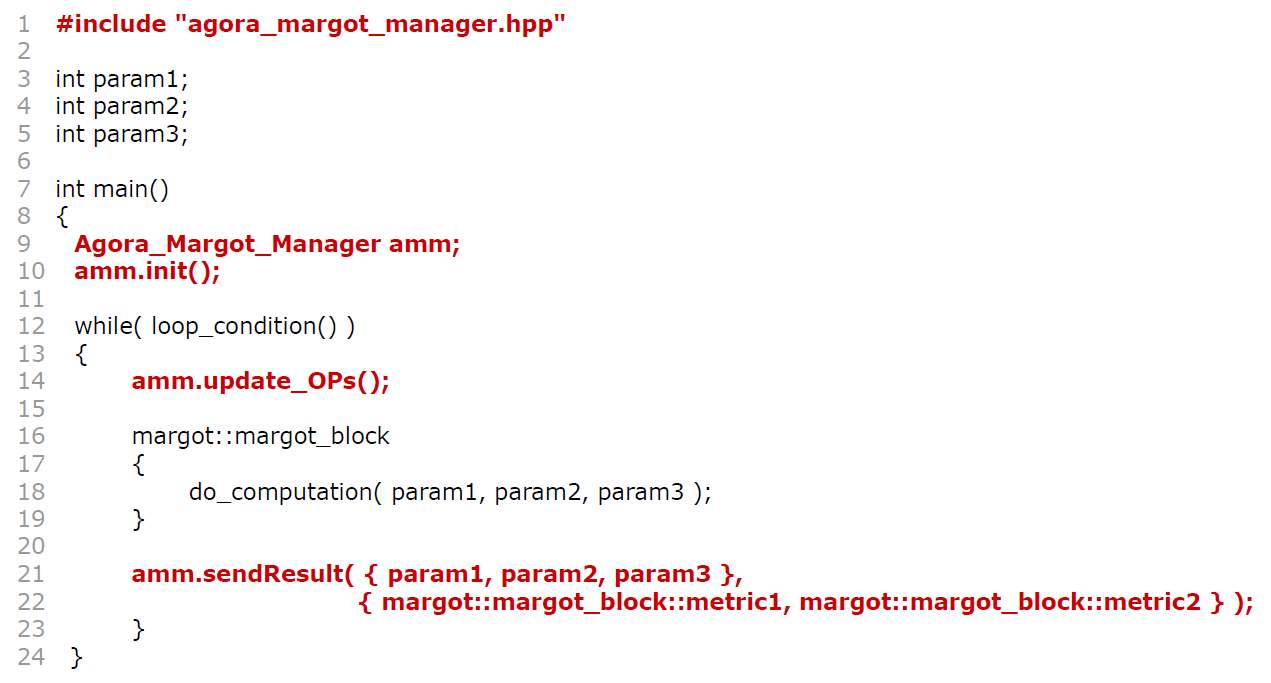
\includegraphics[width = \textwidth]{tesiCris_client_integration}
    \caption{Sketch application with \textit{AgoraLocalAppHandler} module plus mARGOt autotuner integration}
    \label{fig::sketchApp}
    
\end{figure}

Figure \ref{fig::sketchApp} shows a sketch application that, until \textit{loop\_con\-di\-tion()} is verified (line 12), is executed; computation depends on three parameters ($pa\-ram1, pa\-ram2, pa\-ram3$) that are set up by mARGOt autotuner at the beginning of every cycle (line 16), while two metrics of interest ($metric1, metric2$) are monitored (for mARGOt details, see related scientific publication \cite{gadioli2015application}).

Integration code required to use Agora framework with mARGOt autotuner is written in bold red; main steps during program execution are three:

\begin{enumerate}

    \item AgoraLocalAppHandler module and mARGOt autotuner instantiation and initialization (lines 9-10): the AgoraLocalAppHandler module saves all application information and sets up mARGOt autotuner with a default Operating Point; if nothing happens, the application is executed with this configuration;
    
    \item Application knowledge update (line 14): the AgoraLocalAppHandler module updates, from time to time, its internal knowledge about application configurations that are sent by the AgoraRemoteAppHandler module; before mARGOt autotuner sets up application parameters (line 16), AgoraLocalAppHandler checks mARGOt knowledge with respect to its internal one: if they are different, mARGOt Operating Points are updated. In this way, for instance, if the AgoraLocalAppHandler module receives a new configuration during Design Space Exploration phase (see \ref{dse_conf}), mARGOt knowledge is set up with this data, so the application is forced to be executed with the corresponding parameter values; if, for instance, application complete model is received (see \ref{modelSend}), mARGOt internal knowledge is set up with all this information, so the autotuner can choose the best Operating Point that fulfills application current goals and requirements;
    
    \item Operating Point dispatch (line 21-22): after each computation has done, parameter values just used with the corresponding monitored metrics of interest are published on a predetermined MQTT topic, so the related AgoraRemoteAppHandler module can receive this information (see \ref{opSend}).
    
\end{enumerate}

\chapter{Experimental results}\label{exps}

\lettrine{T}{}\textit{o} evaluate the benefits and drawbacks of the Agora framework, we carried out a set of experiments on various applications and scenarios. First, we present the structure of the applications used for the experiments; then, we show the experimental results.

\section{Experimental setup}\label{expSetup}

We evaluate Agora in three different scenarios: two versions of a synthetic application and a real one. This work has been coupled with mARGOt autotuner (\cite{gadioli2015application}). We use the concept of Operating Point (OP) concerning application configurations in terms of parameter values and associated performance (observed metric of interest values).

Synthetic application has three parameters: $param_1$, $param_2$ and $param_3$. A function of these three variables calculates the amount of milliseconds of an execution cycle ($executionTime$ variable), while another function sets up an error measure. This last variable is considered as metric, together with application throughput as number of jobs per second (so, approximately equal to $\dfrac{1000}{executionTime}$).

For the real scenario, Swaptions application is used, taken from the PARSEC benchmark suite (\cite{bienia2008parsec}). This application solves partial differential equations through Monte Carlo simulations in order to price a portfolio of swaptions. Its tunable parameters are: the number of threads (variable $num\_threads$, from 1 to 8) and the number of trials for the simulation at every cycle (variable $num\_trials$, from 100.000 to 1.000.000 with a step of 100.000). Observed metrics of interest are: throughput (variable $avg\_throughput$) as the number of priced swaptions per second and error (variable $avg\_error$), computed as:

\[
avg\_error = \dfrac{\sum_{s \in pricedSwaptions} \left\vert StandDevRef(s) - StandDev(s) \right\vert}{\left\vert pricedSwaptions \right\vert}
\]

where $StandDevRef(s)$ is the reference standard deviation for swaption $s$, $StandDev(s)$ is the evaluated one and $pricedSwaptions$ represents the set of swaptions that are priced at each computing cycle. So, metric $avg\_error$ stands for the average of differences between standard deviation of priced swaptions using evaluated configuration with respect to the reference one (standard deviation for 1.000.000 trials).

Concerning used machine, we run Agora on a Dell XPS 15 9550 with 4 core / 8 threads Intel(R) Core(TM) i7-6700HQ CPU @ 2.60 processor.


\subsection{Synthetic application version 1}

In the first version of synthetic application, the amount of execution time is calculated as:
\[
executionTime = 7.35 \cdot \ln{(param_1)} + 38.1 \cdot param_2 + 52.96 \cdot \sqrt{param_3} + noise
\]

where $noise$ simulates a disturbance. It is computed as:
\[
noise = executionTime \cdot randomNumber \cdot noisePercentage
\]

$randomNumber$ is a generated random value according to an exponential distribution with mean 0.3. $noisePercentage$ affects noise weight and it can be equal to $1\%$, $5\%$, $10\%$, $15\%$, $25\%$ or $50\%$.

Error metric is calculated as:
\[
error = \dfrac{1}{0.015 \cdot \sqrt{param_1} + 0.033 \cdot \ln{(param_2)} + 0.028 \cdot \ln{(param_3)}}
\]

Application parameters can assume these values:

\begin{table}[H]

    \centering

    \begin{tabular}{ll}
    
        \toprule
        Parameters & Values \\
        \midrule
        $param_1$ & 1, 50, 150, 300, 450, 700, 800 \\
        $param_2$ & 1, 50, 100, 150, 200 \\
        $param_3 (\cdot 10)$ & 1, 8, 15, 22, 29, 36, 43, 50, 57, 64, 71, 78, 85 \\
        \bottomrule 
    
    \end{tabular}

    \caption{Synthetic application version 1 parameters and related values}

\end{table}

\begin{figure}[h]

    \centering
    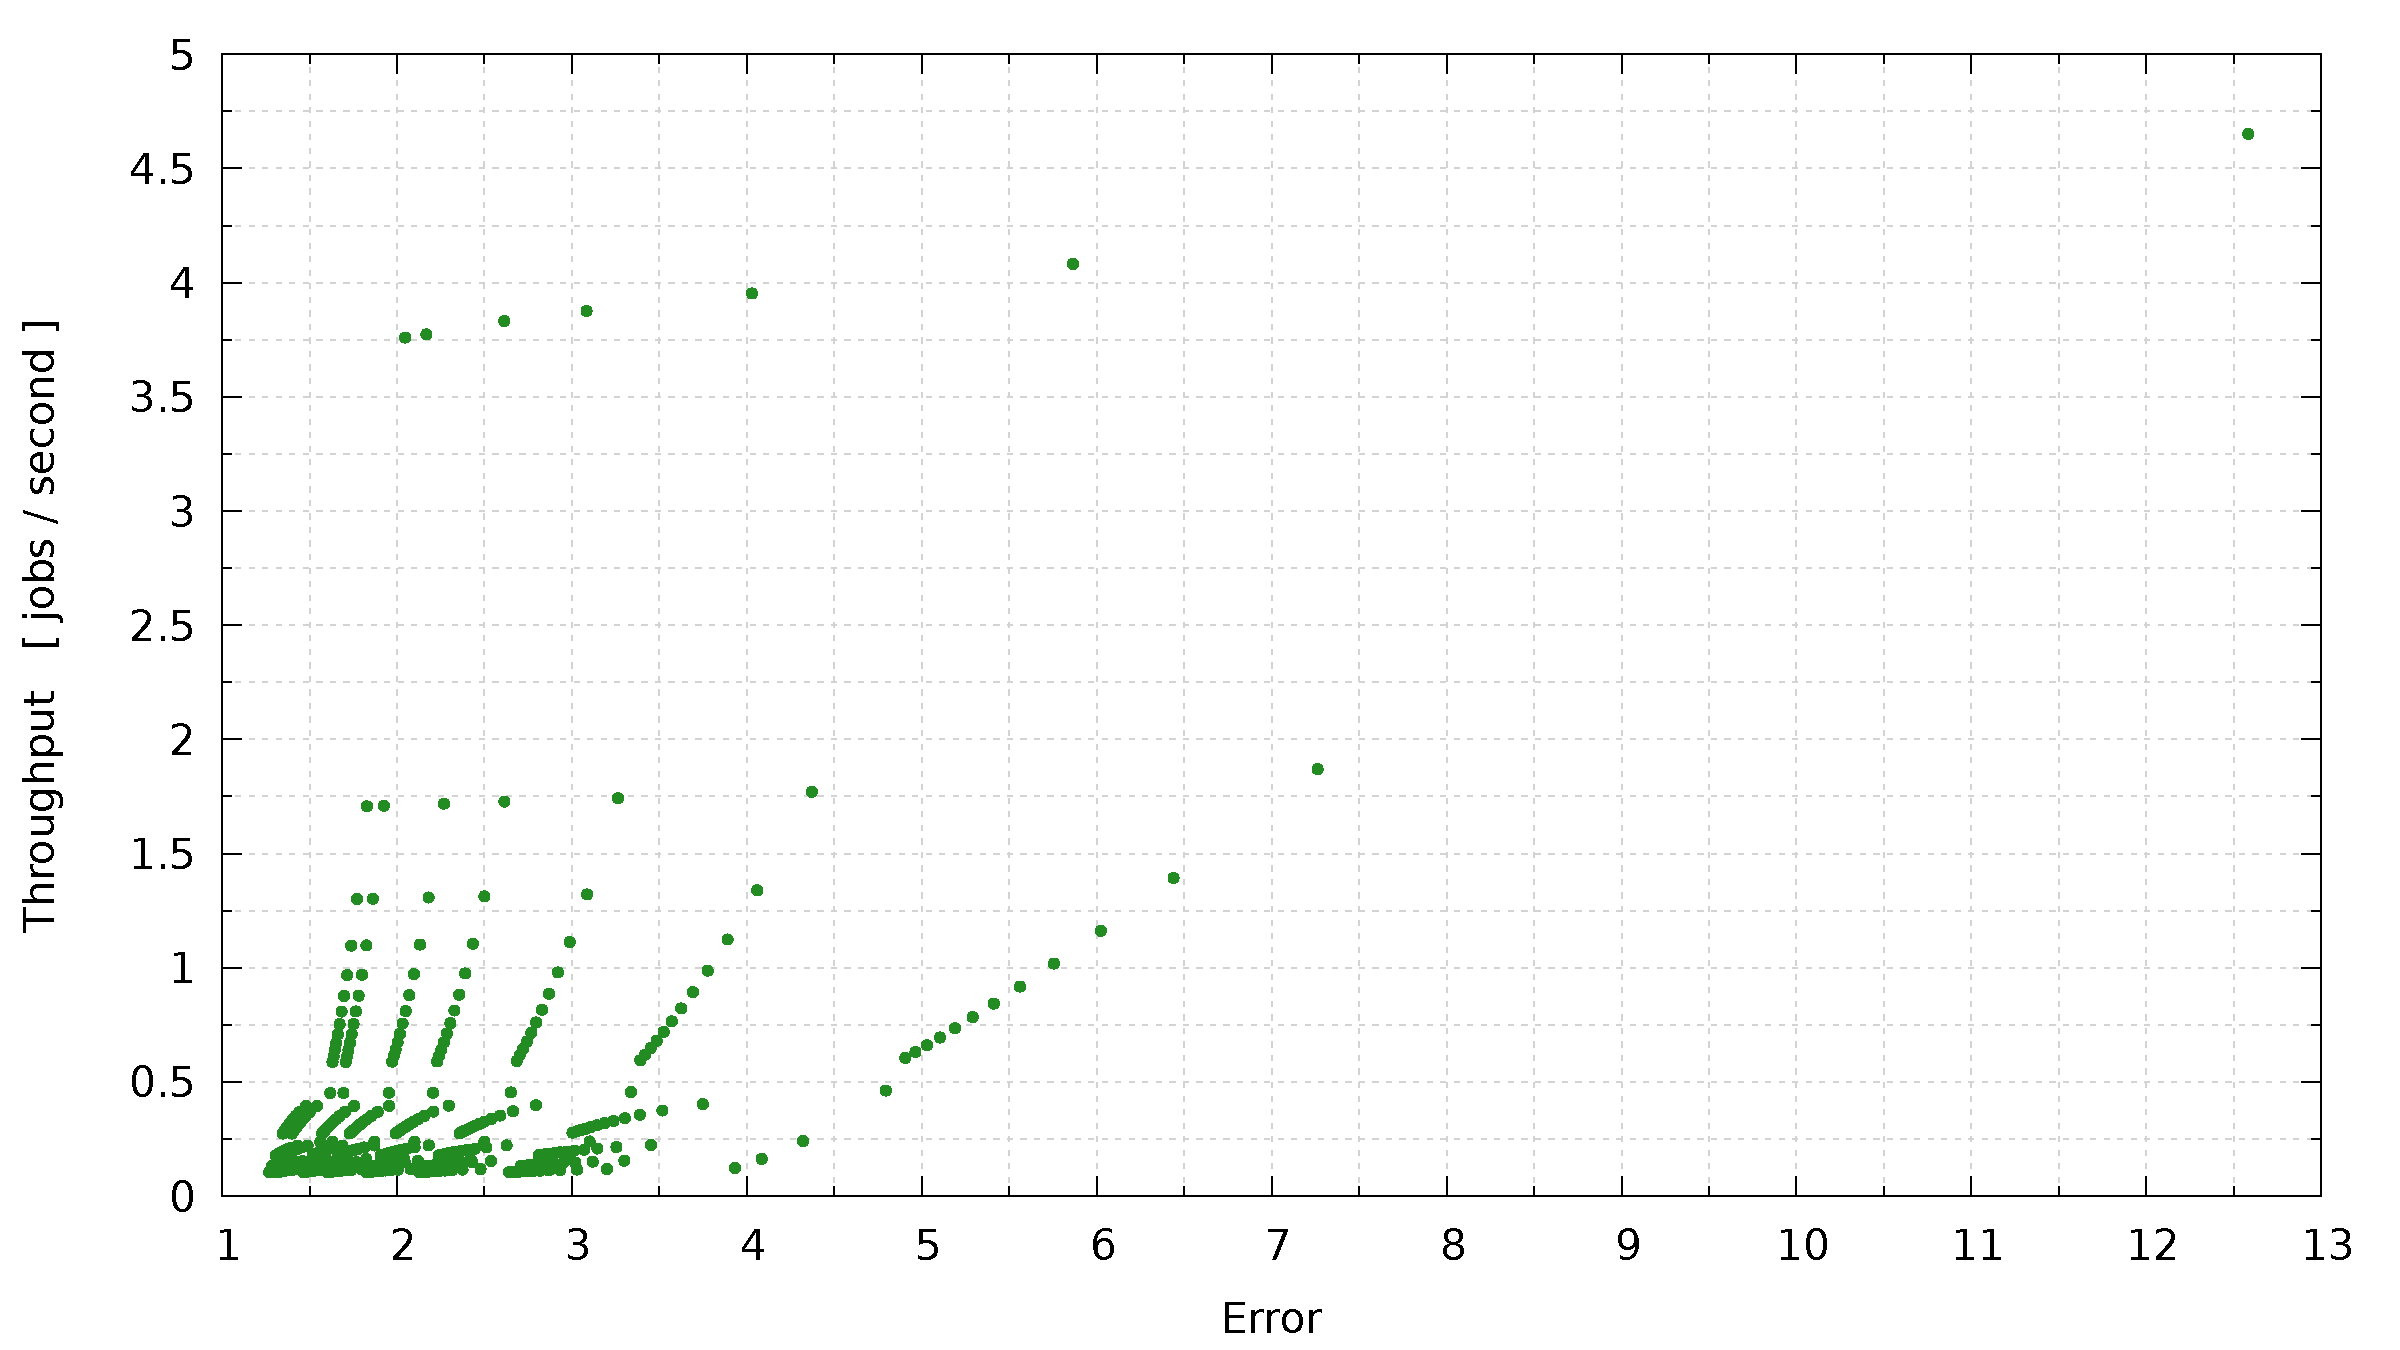
\includegraphics[width = \textwidth]{opGraphSynth1}

    \caption{Throughput by varying the error for synthetic application version 1}

    \label{fig::opListSynth1}
    
\end{figure}

This application has 455 Operating Points. Figure \ref{fig::opListSynth1} shows complete OP distribution for $noisePercentage = 15\%$. Every point stands for a particular configuration with an associated error value (on x-axis) and a throughput one (on y-axis). Since $noise$ in $executionTime$ is affected by $randomNumber$, this plot consider its expected value, equal to the mean of the chosen exponential distribution (0.3). The obtained OP list represents the reference model for this predetermined $noise\-Per\-cent\-age$ value. Other reference models are similar, since the only difference is the $noisePercentage$ value for the calculation of $executionTime$ variable.

Concerning model prediction quality, therefore, for every application setting with a fixed $noisePercentage$, estimated OP list is compared with the corresponding reference one.


\subsection{Synthetic application version 2}

\begin{figure}[h	]

    \centering
    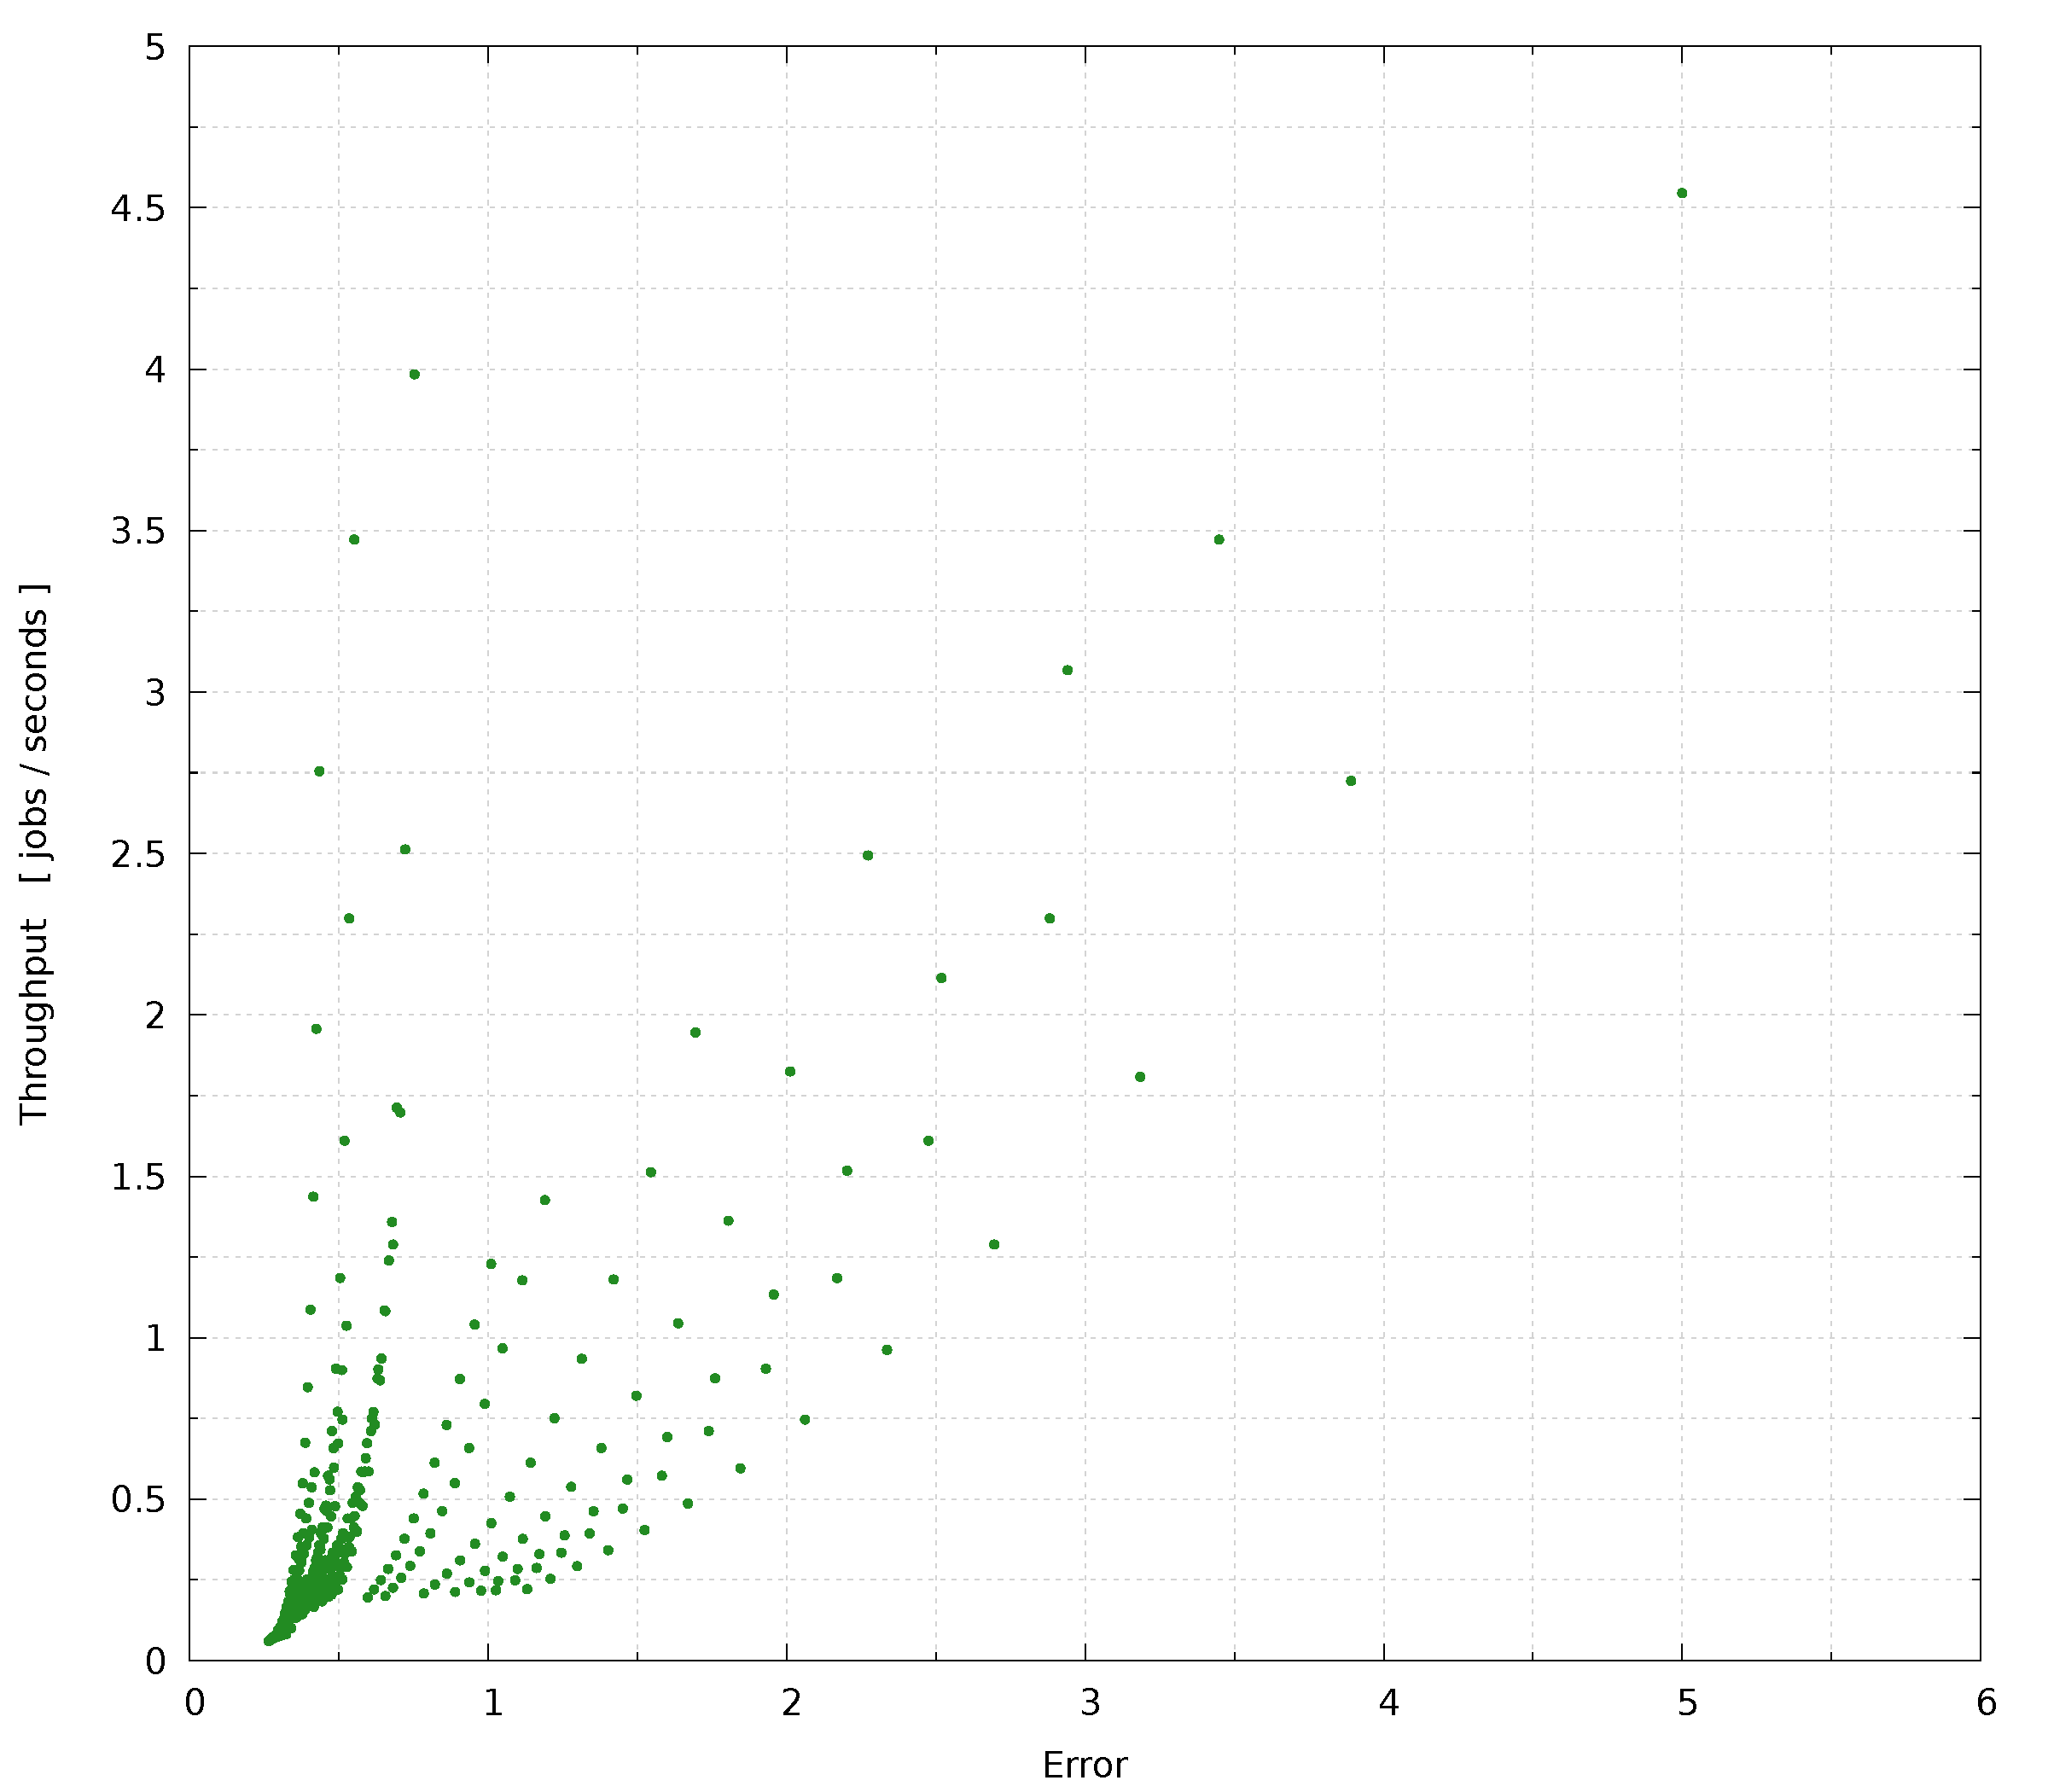
\includegraphics[width = \textwidth]{opGraphSynth2}

    \caption{Throughput by varying the error for synthetic application version 2}
 
   \label{fig::opListSynth2}
    
\end{figure}

In the second synthetic application version, execution time is equal to:
\[
executionTime = 7.4 \cdot param_1 \cdot param_2 + 2.1 \cdot (param_3)^2 + noise
\]

where $noise$ is simulated as in the previous application version, while the error is:

\[
error = \dfrac{1}{0.01 \cdot param_1 + 0.7 \cdot \ln{(param_2)} + 0.019 \cdot param_3}
\]

Parameter values are:

\begin{table}[H]

    \centering

    \begin{tabular}{ll}
    
        \toprule
        Parameters & Values \\
        \midrule
        $param_1$ & 1, 10, 15, 25, 40, 65, 80 \\
        $param_2$ & 1, 5, 10, 20 \\
        $param_3$ & 10, 13, 16, 19, 22, 25, 28, 31, 34, 37, 40, 43, 46 \\
        \bottomrule 
    
    \end{tabular}

    \caption{Synthetic application version 2 parameters and related values}

\end{table}

In this application the number of Operating Points is 364. Figure \ref{fig::opListSynth2} shows complete OP distribution of reference model with $noise\-Per\-cent\-age = 5\%$. Every point stands for a particular configuration with an associated error value (on x-axis) and a throughput one (on y-axis).

Regarding model prediction goodness, same reasoning as previous application version is applied.


\subsection{Swaptions}

This application has two parameters: $num\_\-threads$ and $num\_\-trials$. Their values are:

\begin{table}[H]

    \centering

    \begin{tabular}{ll}
    
        \toprule
        Parameters & Values \\
        \midrule
        $num\_threads$ & 1, 2, 3, 4, 5, 6, 7, 8 \\
        $num\_trials (\cdot 10^3)$ & 100, 200, 300, 400, 500, 600, 700, 800, 900, 1000 \\
        \bottomrule 
    
    \end{tabular}

    \caption{Swaptions parameters and related values}

\end{table}

The number of Operating Points is therefore 80. Figure \ref{fig::swaptionsOPs} shows complete OP distribution with respect $avg\_error$ and $avg\_throughput$ metrics of interest.

\begin{figure}[ht]

    \centering

    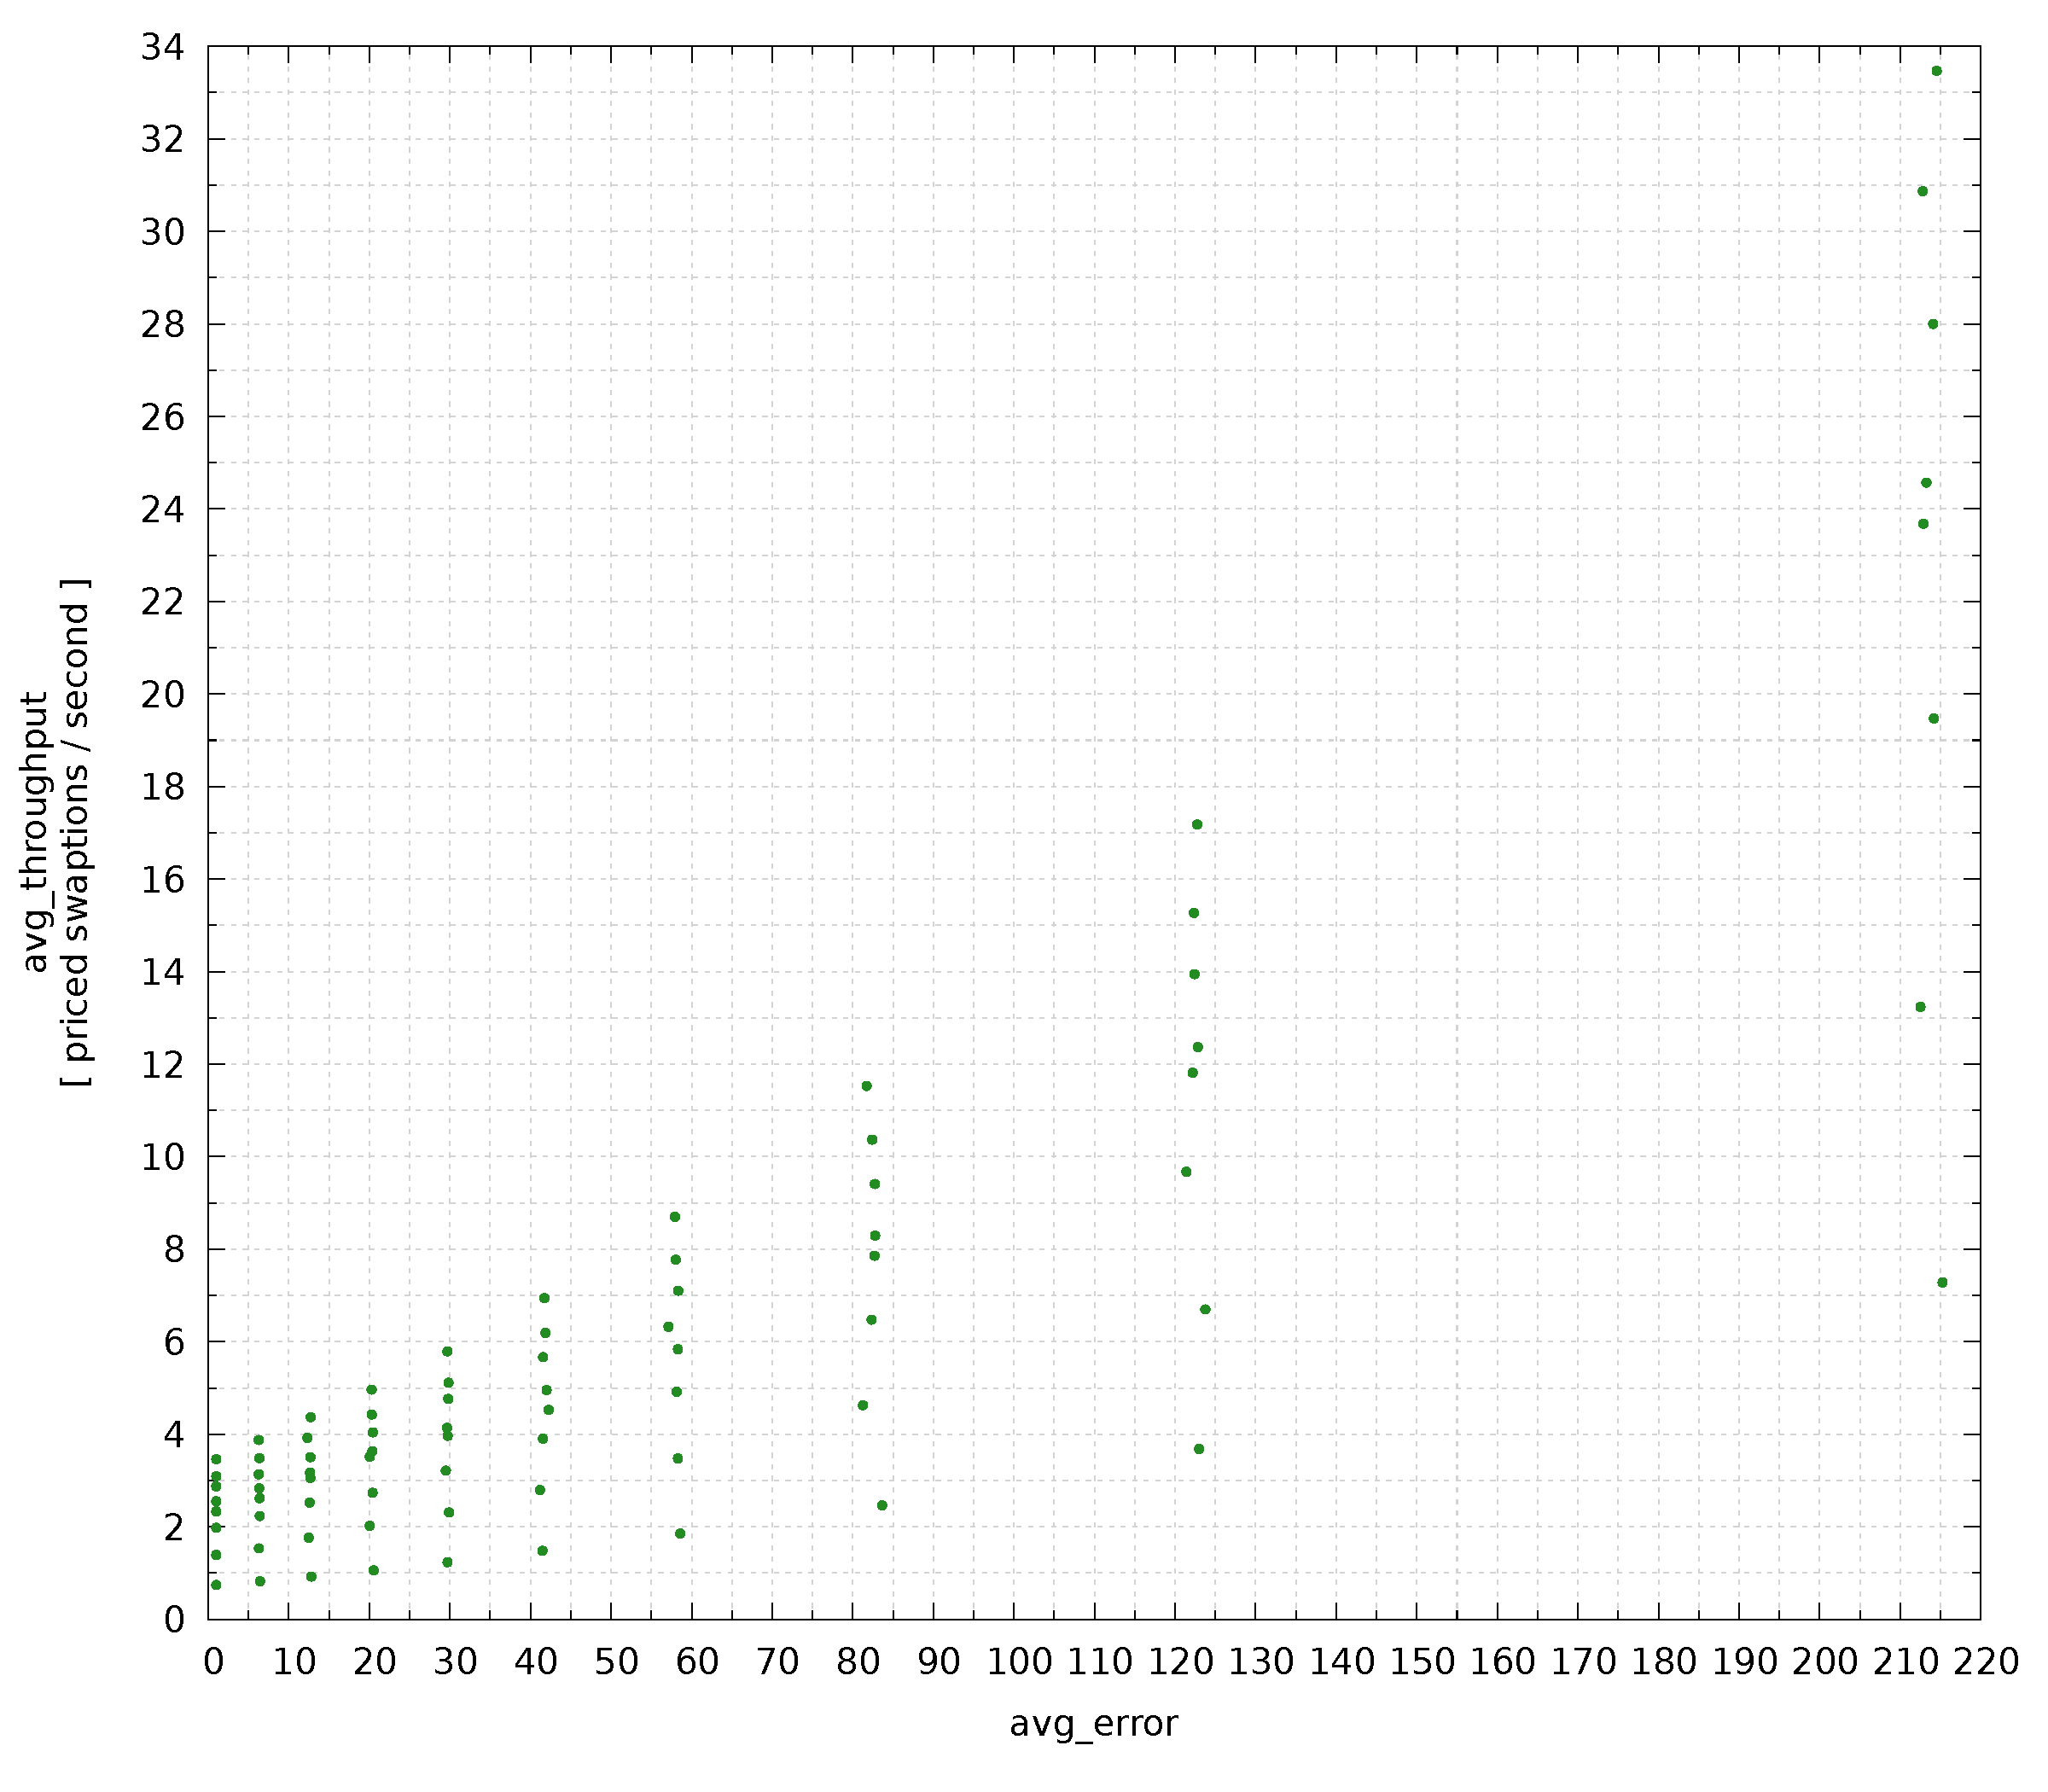
\includegraphics[width = \textwidth]{swaptionsOPgraph}

    \caption{Average throughput by varying the average error for Swaptions}

    \label{fig::swaptionsOPs}
    
\end{figure}





\section{Experimental campaign}\label{campaign}

We want to demonstrate Agora validity. For both synthetic application versions and Swaptions, we focuse our attention on model prediction goodness in various scenarios. We study execution times, especially for Design Space Exploration phases with one and more than one executing applications at the same time, highlighting benefits in sharing DSE. We reveal application behavior during execution on different cases. Next paragraphs show results, firstly for synthetic applications, finally for the real one.


\subsection{Synthetic application}

In this paragraph we show experimental results for both versions of synthetic application, divided as explained before.


\subsubsection{Model prediction quality}\label{deltaErrorExplanation}

Concerning model prediction goodness, both synthetic application versions are executed several times with the introduction of all noise weights ($1\%$, $5\%$, $10\%$, $15\%$, $25\%$ and $50\%$), focusing on the prediction of throughput metric, that is the one affected by $noise\-Percentage$ value. A Face Centered Central Composite Desing of Experiments with one Center Point has been used, firstly gathering 1 repetition, then 5 repetitions and finally 10 repetitions for each DoE configuration during Design Space Exploration phase. For each predicted metric value $m$ for each application setting, we have calculated a $deltaError$ measure:

\[
deltaError(m) = \dfrac{\left\vert predictedValue(m) - referenceValue(m) \right\vert \cdot 100}{\left\vert referenceValue(m) \right\vert}
\]

where $predictedValue(m)$ and $referenceValue(m)$ have explicit meaning. So, $deltaError(m)$ stands for how much the predicted metric value $m$ distances itself from the corresponding value of the related reference model, in percentage. Figures from \ref{fig::synth1spark1::intervals} to \ref{fig::synth2spark2::means} summarize results.





\begin{figure}[htb]

    \centering
    
    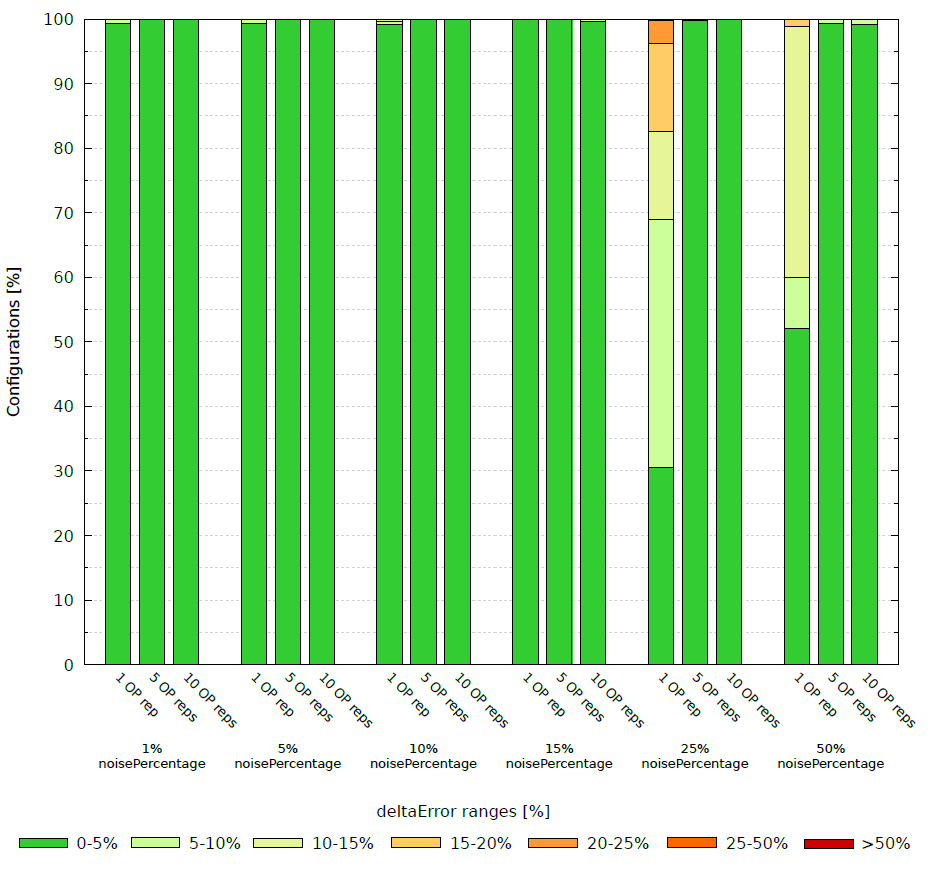
\includegraphics[width = \textwidth]{deltaErrorRangesSynth1spark1PNG}
    
     \caption{$deltaError$ results for throughput metric of synthetic application version 1 by varying the noisePercentage and the number of OP repetitions. Used RSM: 1st version of implemented GLR ("transformations by functions")}
    
    \label{fig::synth1spark1::intervals}
    
\end{figure}

\begin{figure}[htb]

    \centering
    
    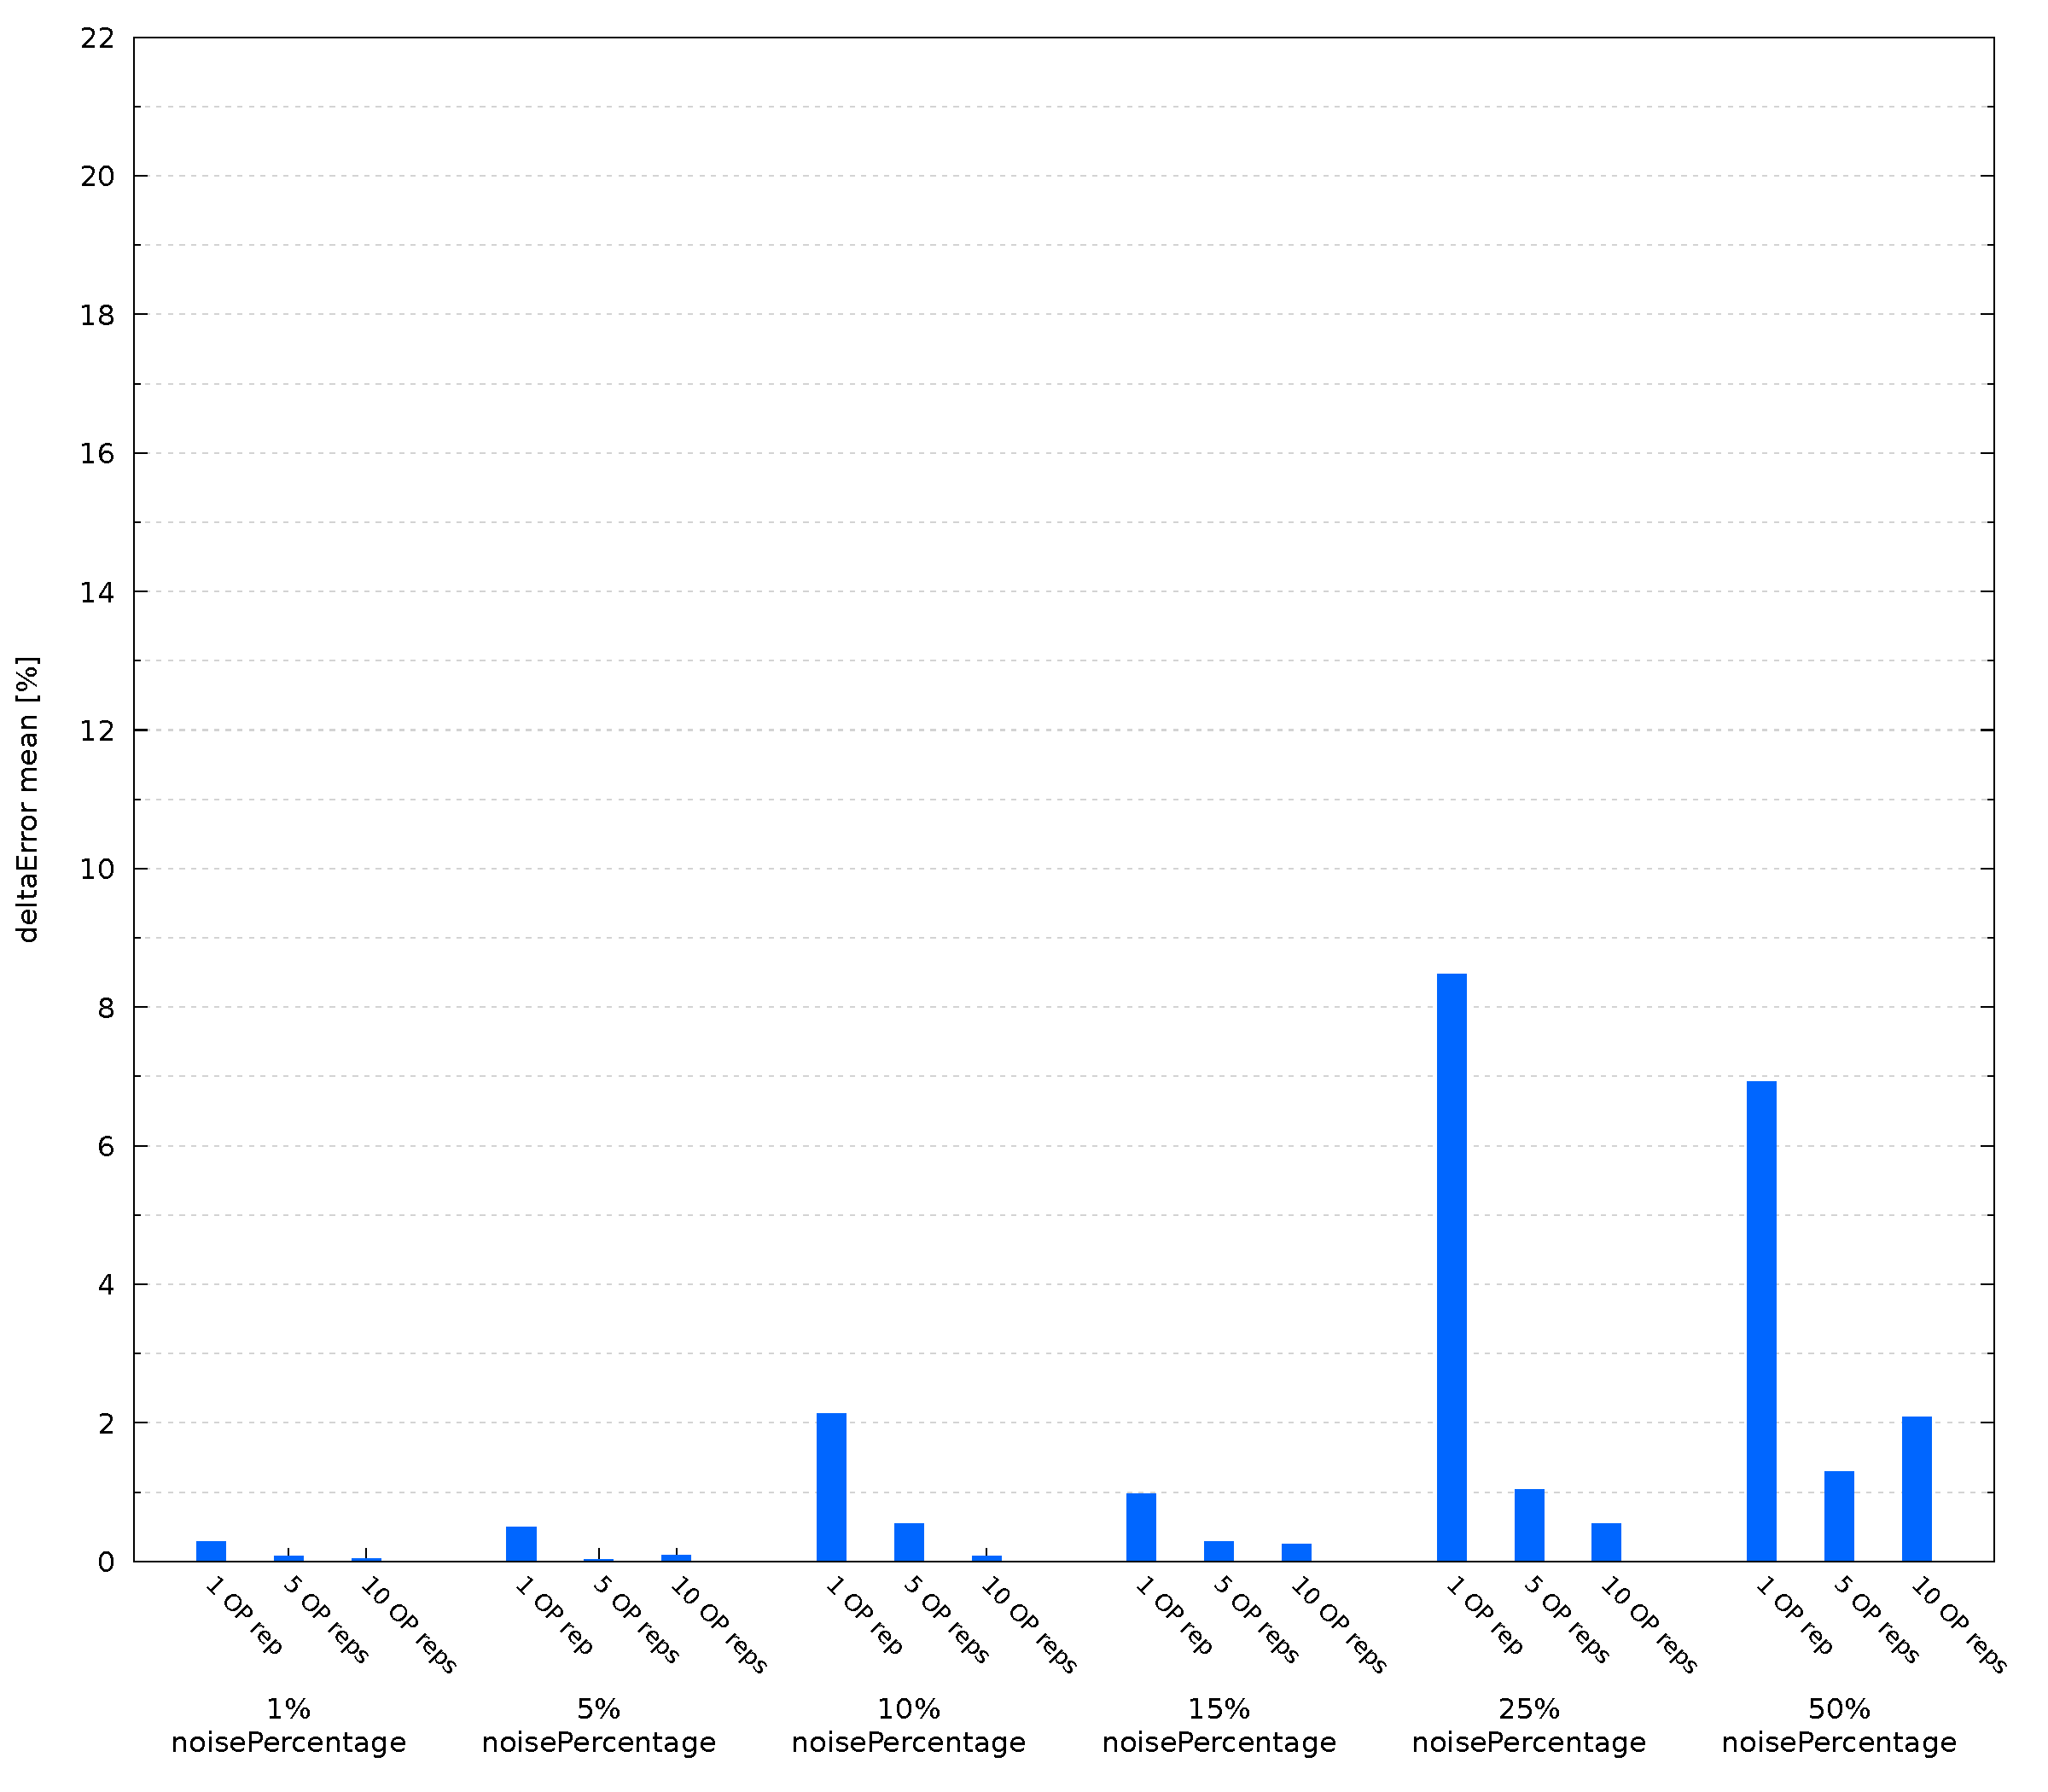
\includegraphics[width = \textwidth]{deltaErrorMeansSynth1spark1}
    
    \caption{$deltaError$ mean for throughput metric of synthetic application version 1 by varying the noisePercentage and the number of OP repetitions. Used RSM: 1st version of implemented GLR ("transformations by functions")}
    
    \label{fig::synth1spark1::means}
    
\end{figure}





\begin{figure}[htb]

    \centering
    
    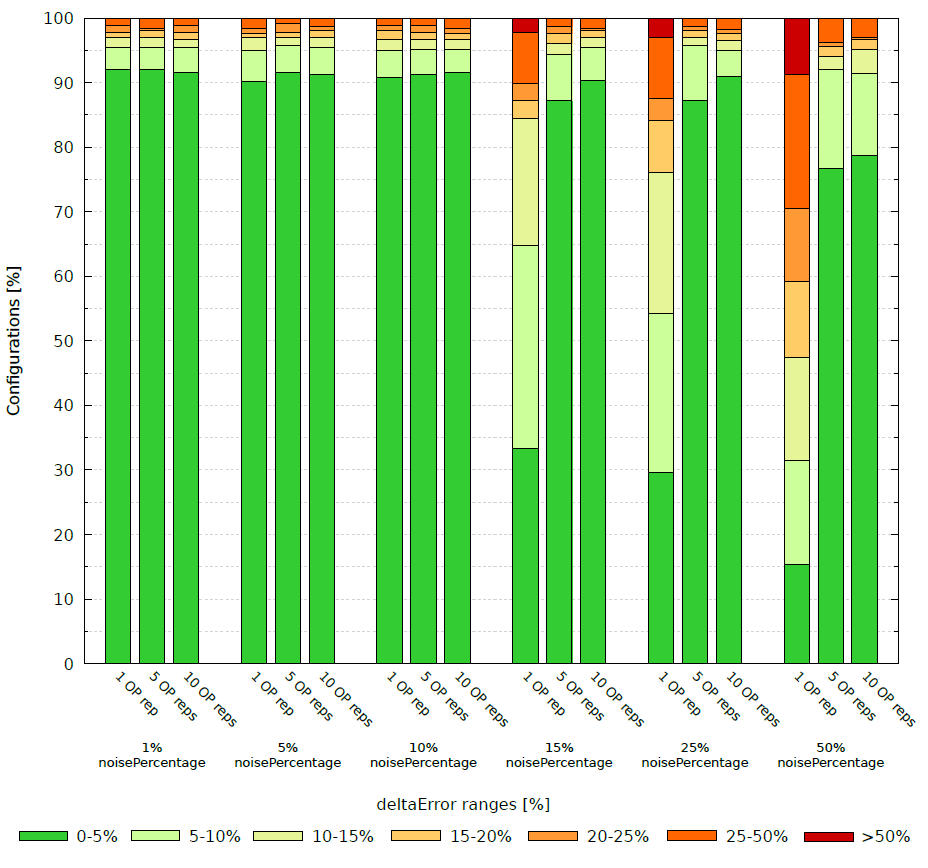
\includegraphics[width = \textwidth]{deltaErrorRangesSynth1spark2PNG}
    
     \caption{$deltaError$ results for throughput metric of synthetic application version 1 by varying the noisePercentage and the number of OP repetitions. Used RSM: 2nd version of implemented GLR ("polynomial combinations of degree 2")}
    
    \label{fig::synth1spark2::intervals}
    
\end{figure}

\begin{figure}[htb]

    \centering
    
    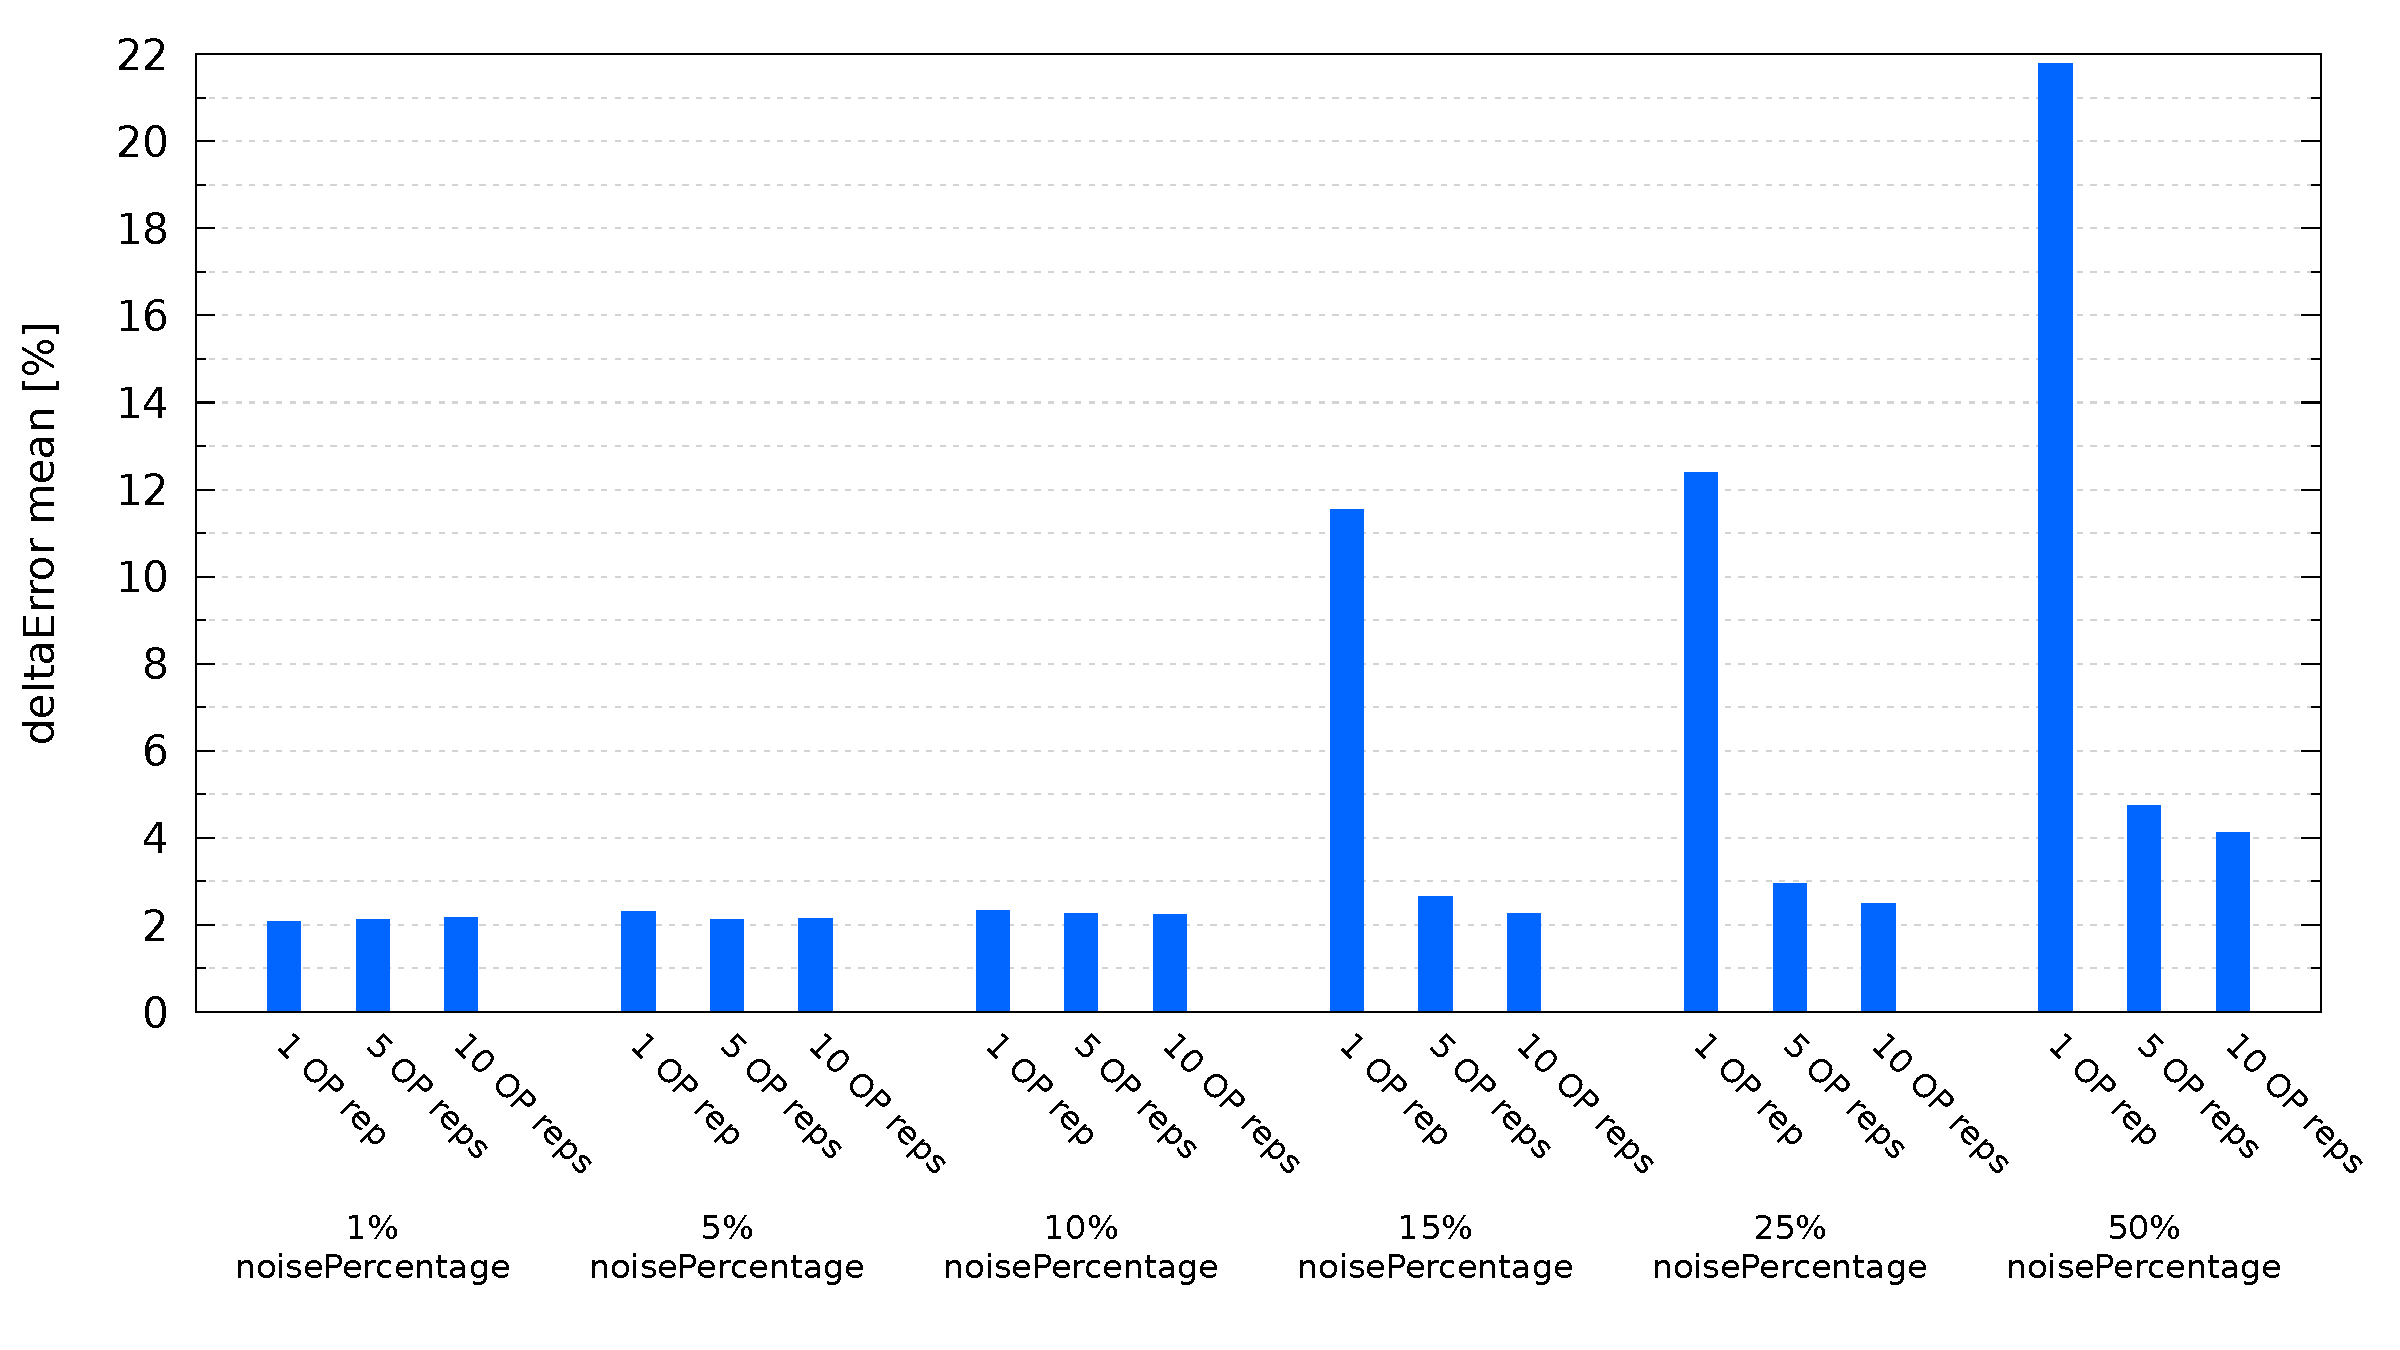
\includegraphics[width = \textwidth]{deltaErrorMeansSynth1spark2}
    
    \caption{$deltaError$ mean for throughput metric of synthetic application version 1 by varying the noisePercentage and the number of OP repetitions. Used RSM: 2nd version of implemented GLR ("polynomial combinations of degree 2")}
    
    \label{fig::synth1spark2::means}
    
\end{figure}





\begin{figure}[htb]

    \centering
    
    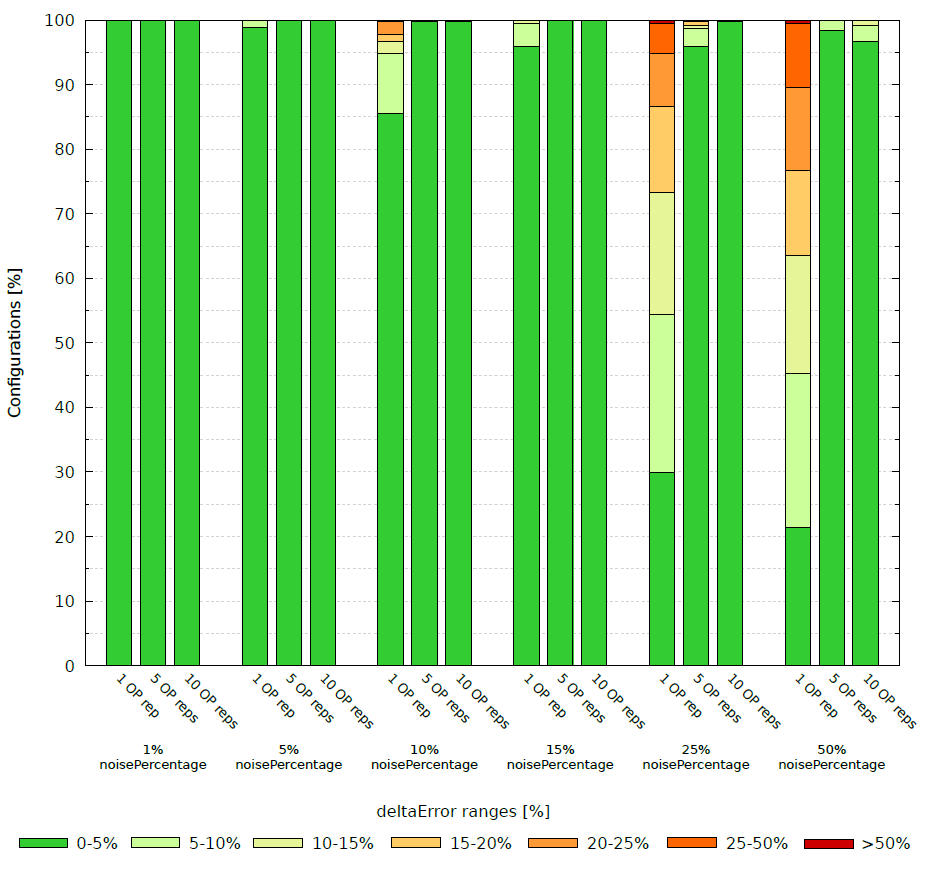
\includegraphics[width = \textwidth]{deltaErrorRangesSynth2spark2PNG}
    
     \caption{$deltaError$ results for throughput metric of synthetic application version 2 by varying the noisePercentage and the number of OP repetitions. Used RSM: 2nd version of implemented GLR ("polynomial combinations of degree 2")}
    
    \label{fig::synth2spark2::intervals}
    
\end{figure}

\begin{figure}[htb]

    \centering
    
    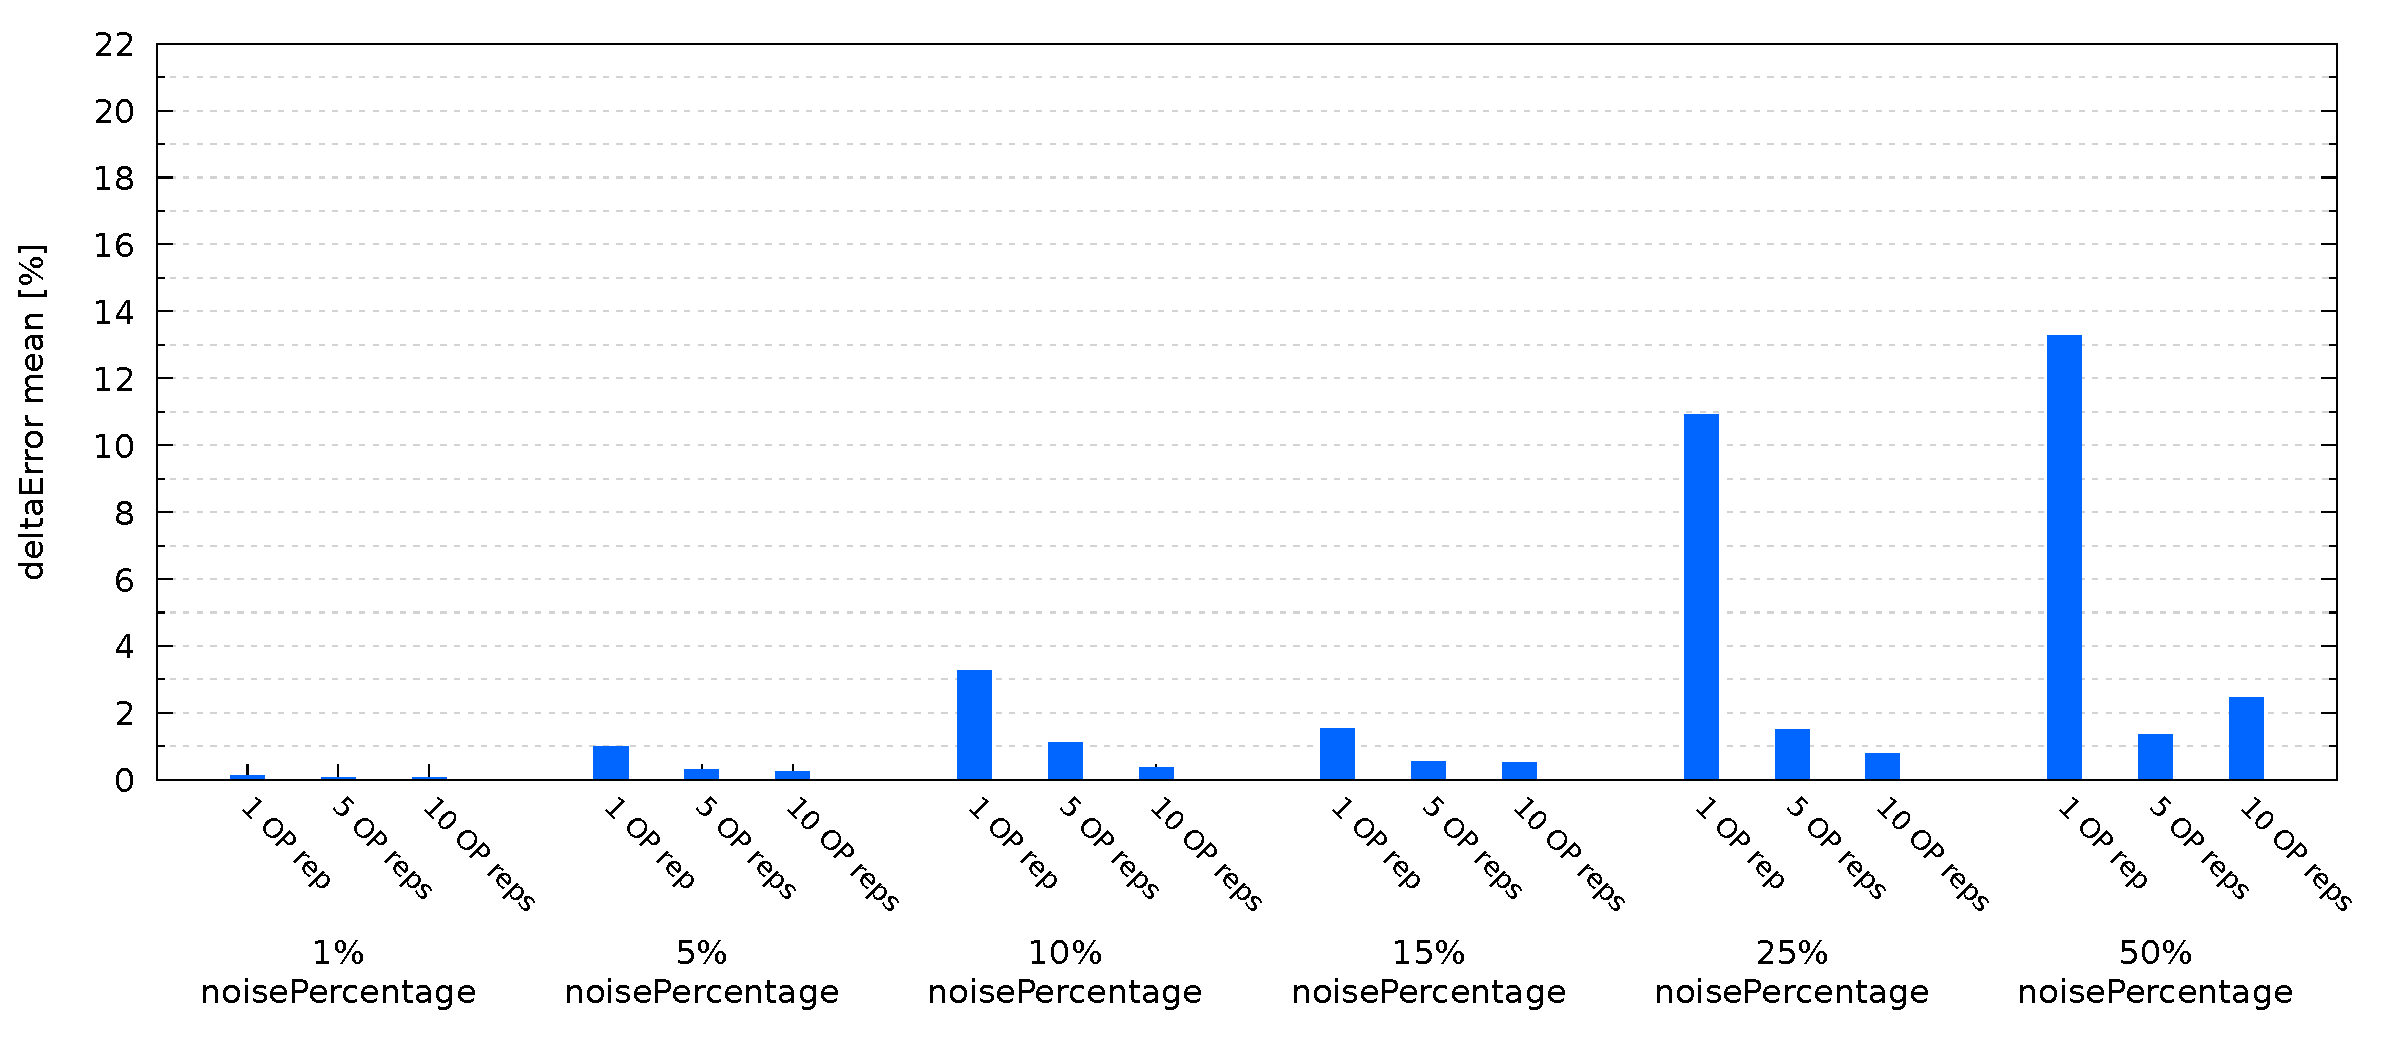
\includegraphics[width = \textwidth]{deltaErrorMeansSynth2spark2}
    
    \caption{$deltaError$ mean for throughput metric of synthetic application version 2 by varying the noisePercentage and the number of OP repetitions. Used RSM: 2nd version of implemented GLR ("polynomial combinations of degree 2")}
    
    \label{fig::synth2spark2::means}
    
\end{figure}





In Figures \ref{fig::synth1spark1::intervals}, \ref{fig::synth1spark2::intervals} and \ref{fig::synth2spark2::intervals}, each stacked bar chart represent an application setting with respect to $noisePercentage$ value and the number of repetitions, for each DoE configuration, collected during DSE phase; on y-axis there are the number of predicted OPs, in percentage, grouped with respect to measured $deltaError$ of related throughput metric. Related Figures \ref{fig::synth1spark1::means}, \ref{fig::synth1spark2::means} and \ref{fig::synth2spark2::means} show $deltaError$ mean for each program setting.

From Figure \ref{fig::synth1spark1::intervals} we can see that, until $noisePercentage = 15\%$, model prediction is really precise even with only 1 repetition for each DoE configuration: almost the totality of OPs have a $del\-ta\-Er\-ror$ below $5\%$. With 5 repetitions and 10 repetitions, all configurations have a $del\-ta\-Er\-ror$ below $5\%$. With the introduction of a strong noise weight, $25\%$ and $50\%$, prediction get worse with 1 OP repetition, even if, respectively, around $70\%$ and $60\%$ of configurations remains with a $deltaError$ below $10\%$. Prediction gets back really accurate with 5 and 10 OP repetitions also with these high noise values.

Figure \ref{fig::synth1spark2::intervals} shows that, for synthetic application 1, 2nd version of the implemented GLR produces, in general, results less precise that the ones generated with the 1st GLR version: up to $noisePercentage = 10\%$, quality of predicted models is very satisfying, where more than $90\%$ of OPs have a $deltaError$ below $5\%$. From noise weight equal to $15\%$, $25\%$, $50\%$ and with 1 OP repetition, this $deltaError$ percentage decreases to $35\%$, $30\%$ and $15\%$ respectively and a visible number of Operating Points has a $deltaError$ greater that $25\%$. For these settings, model prediction quality remarkably increases collecting more training data for each Design of Experiments configuration: with 5 and 10 OP repetitions we notice very few predicted OPs with a $deltaError$ greater that $10\%$, so prediction quality becomes very accurate even in these awful cases.

Concerning synthetic application version 2 with the 2nd version of implemented Generalized Linear Regression as RSM (Figure \ref{fig::synth2spark2::intervals}), results are very similar to the ones related to synthetic application version 1 with 1st version of implemented Generalized Linear Regression (Figure \ref{fig::synth1spark1::intervals}): quality of model prediction is generally very high, even with heavy noises but, in these cases, there is the need of more OP repetitions in order to mitigate this strong disturbance.

For synthetic application version 1, as it can be understood, 1st implemented version of GLR works slightly better than the 2nd one, but their prediction times are very different, as shown in Table \ref{tab::GLRtimes}.

\begin{table}[htb]

    \centering
    
    \begin{tabular}{cccc}
    
        \toprule
         & 1 OP rep & 5 OP reps & 10 OP reps \\
        \midrule
        GLR 1st version & 155.52 sec & 155.7 sec & 157.72 sec \\
        GLR 2nd version & 23.21 sec & 23.64 sec & 23.8 sec \\
        \bottomrule 
    
    \end{tabular}

    \caption{Model prediction time by varying Generalized Linear Regression strategy and the number of OP repetitions}
    \label{tab::GLRtimes}
    
\end{table}

2nd GLR version takes less than 24 seconds to predict complete model, while 1st GLR version approximately 156 seconds: the former, almost to the same level of quality, is more than 6 times faster than the latter. Moreover, we have noticed that the number of OP repetitions affects very poorly model prediction time; from Table \ref{tab::GLRtimes} we can understand that, among 1, 5 and 10 OP repetitions for each DoE configuration case, times vary very few.

We have not disclosed model prediction quality for synthetic application version 2 with the 1st implemented version of GLR: "transformations by functions" strategy is not able to capture functions of second order behavior, as variable $executionTime$ is built in this case. On the contrary, "polynomial combinations of degree 2" technique has the capability to highly predict functions with, for instance, logarithmic or square root values, as demonstrated in the second model prediction analysis (Figure \ref{fig::synth1spark2::intervals}).

From last analyses, we can assert that Generalized Linear Regression with "polynomial combinations of degree 2" is a Response Surface Methodology much more powerful than GLR that uses "transformations by functions": the latter version can predict a restricted set of scenarios, while the former is able to include those cases and the wide variety of quadratic functions. Agora has been able to predict very well these metric behaviors and to properly manage strong noise disturbances, with the necessity to do, in some cases, a longer Design Space Exploration phase, collecting more OPs for each Design of Experiments configuration. Lastly, Figures \ref{fig::synth1spark1::means}, \ref{fig::synth1spark2::means} and \ref{fig::synth2spark2::means} recap all various scenarios, showing $deltaError$ mean values that increase with high noises, going back still very low with 5 and 10 OP repetitions, even in the worst cases.


\subsubsection{Execution times}

Concerning execution times, we want to show the significant benefit of sharing Design Space Exploration phase among several nodes, running the same application. The 2nd version of synthetic application with $noise\-Percentage = 10\%$ is executed, using Face Centered Central Composite Desing of Experiments with one Center Point and collecting, for each configuration, 20 repetitions. For this application setting, the total number of configurations to be explored is 300. We accomplish this DSE phase with 1 up to 10 executing applications, collecting the overall executing time, represented by each bar chart in Figure \ref{fig::DSEtimes}.

\begin{figure}[htb]

    \centering
    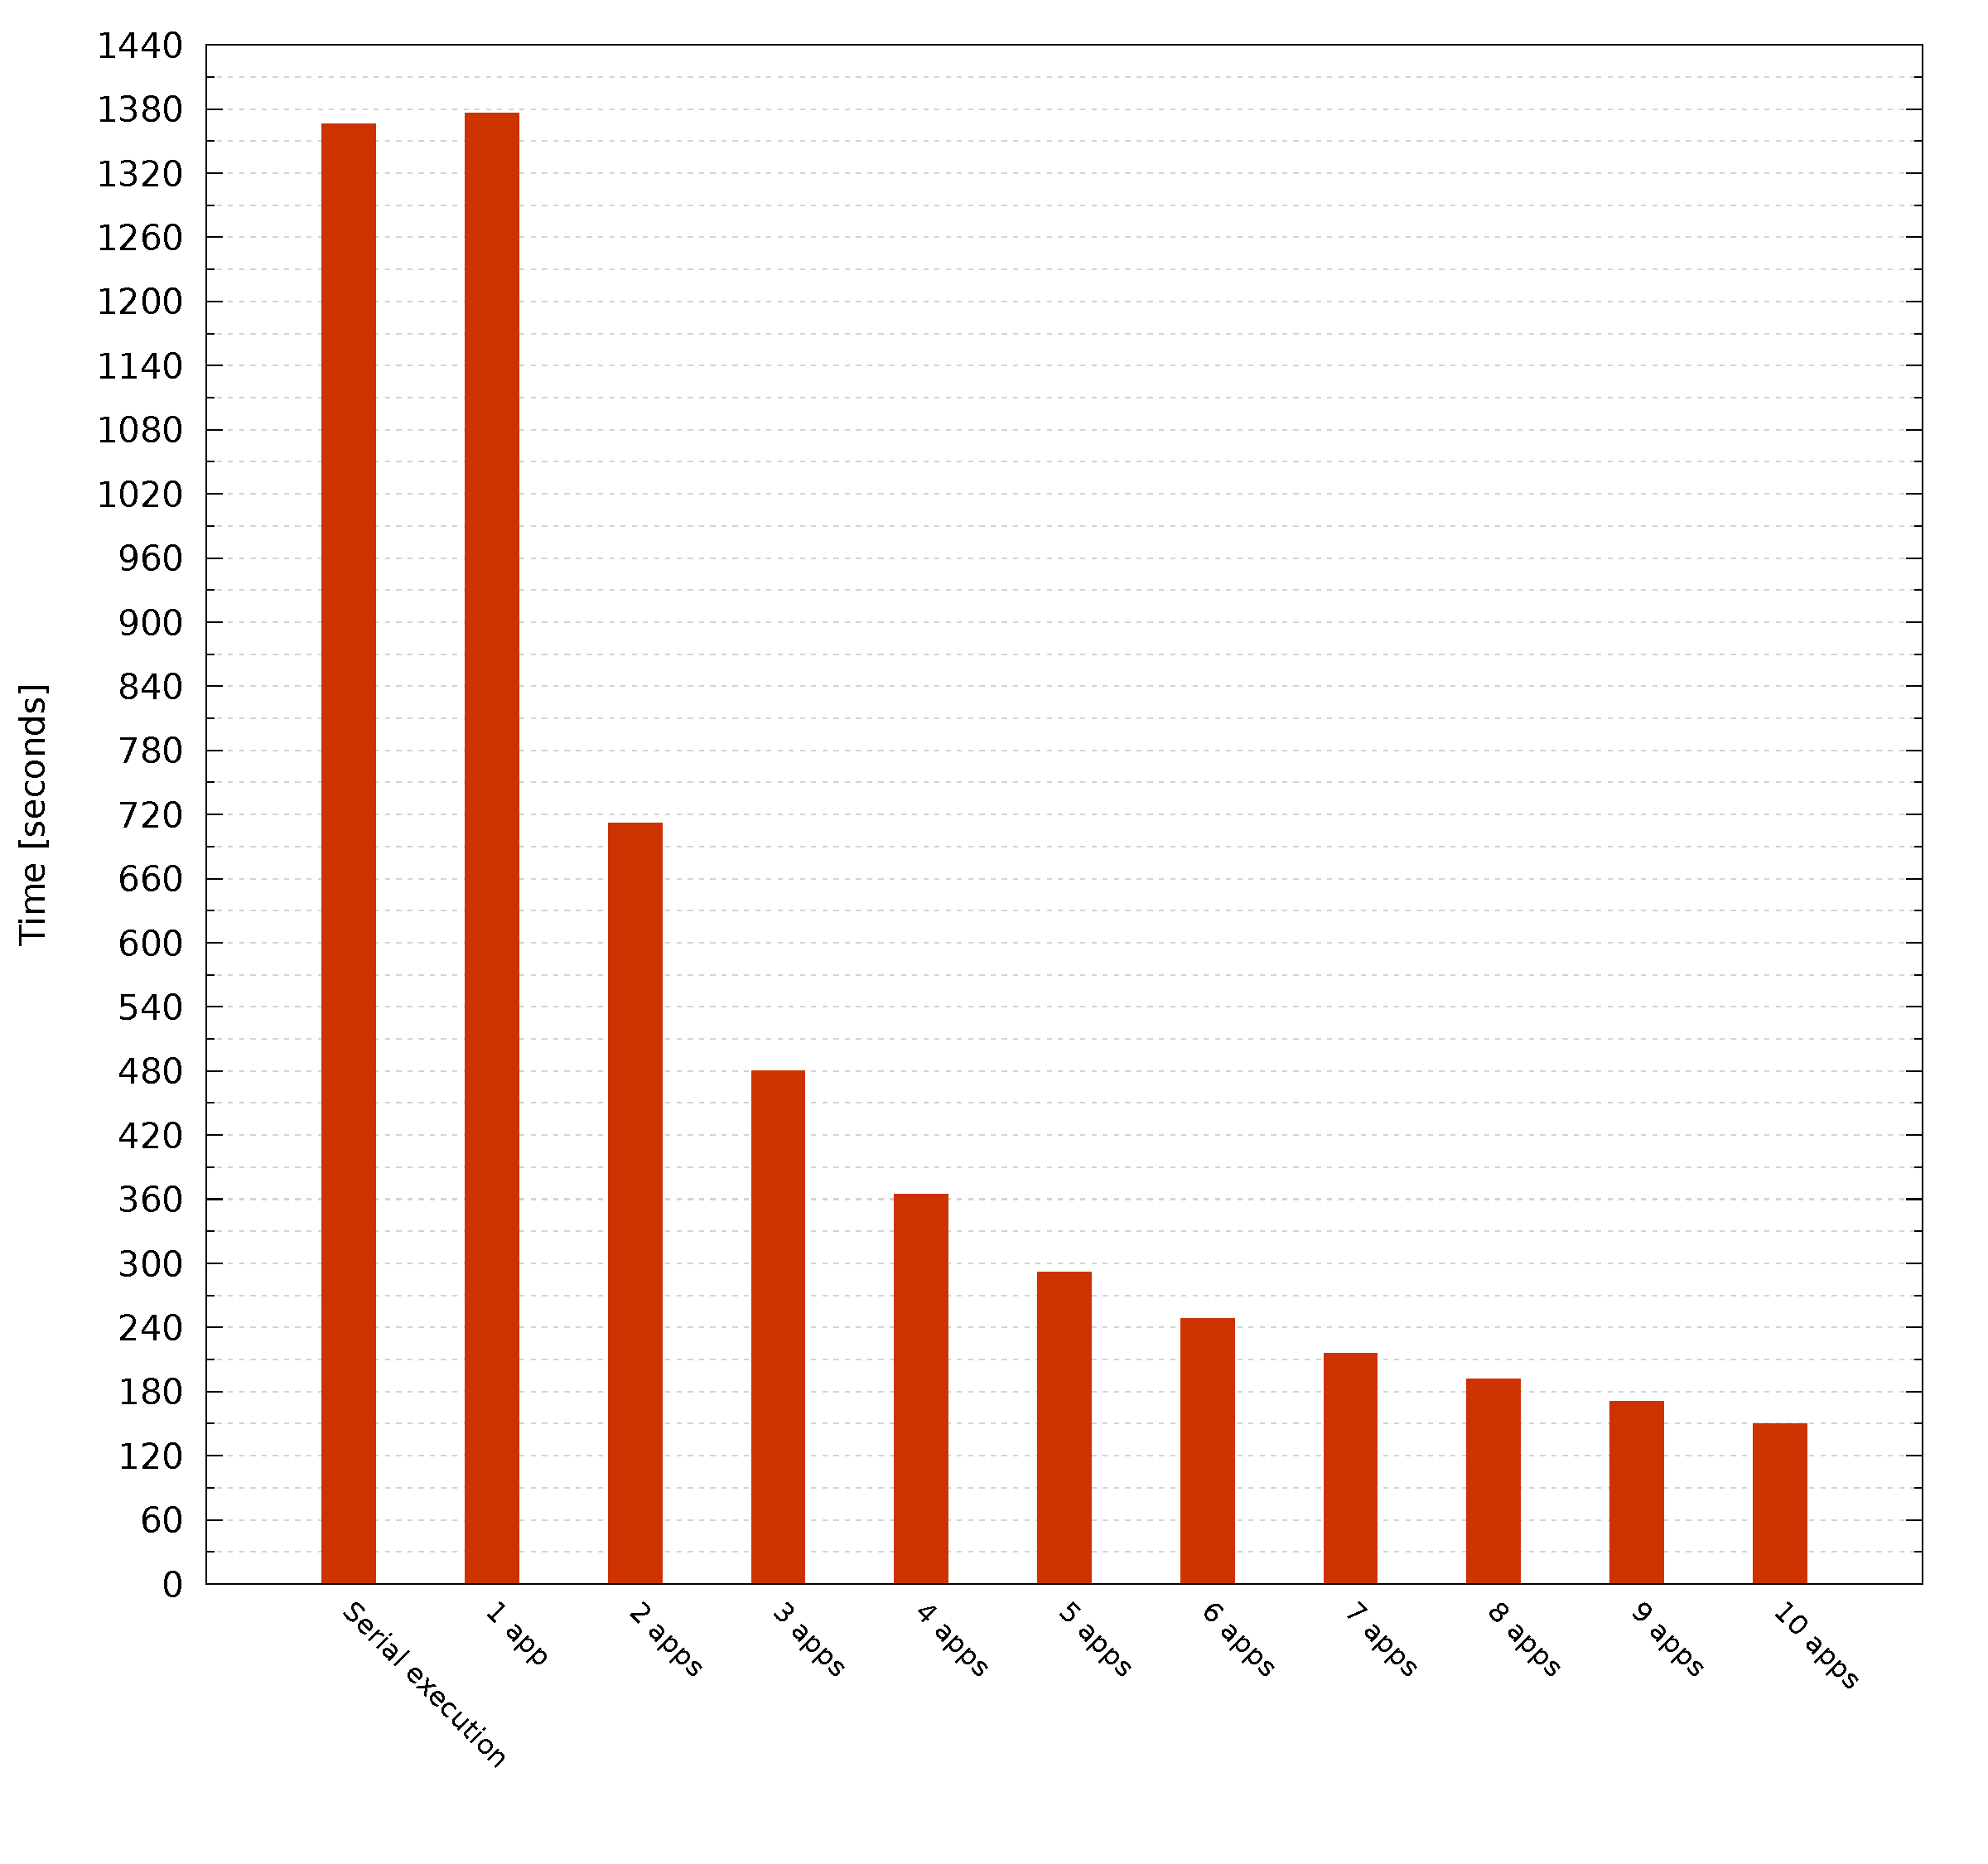
\includegraphics[width = \textwidth]{DSEtimes}
    \caption{Design Space Exploration time by varying the number of executing applications}
    \label{fig::DSEtimes}
    
\end{figure}

From Figure \ref{fig::DSEtimes} we can see that Agora takes about 23 minutes to terminate Design Space Exploration with 1 executing application (second bar chart). The first bar chart shows the amount of time needed to execute application with all the 300 configurations in a serial way, without Agora; this execution lasts around 10 seconds less than the first analyzed scenario, due to the lack of Agora overheads. As we can understand, they are in any case very little: they add only approximately $0.73\%$ of time with respect of the serial execution. From 2 executing applications on, DSE time strongly decreases: Agora takes around 12 minutes to finish this phase with just 2 executing applications, 8 minutes with 3 ones, up to only 2 and a half minutes with 10 ones, more than 9 times lower than DSE phase with 1 application. Sharing Design Space Exploration phase among more than one executing application clearly speeds up overall time, since collection of training data duration, that is much longer than model prediction one (reported in Table \ref{tab::GLRtimes}), considerably goes down.

Now we want to show general Agora advantages, comparing a Full-Factorial, so exhaustive, application execution with the one supervised by this work. In Figure \ref{fig::full_cris}, first bar chart shows overall time needed to compute Full-Factorial run for synthetic application version 2 with $noisePercentage = 15\%$, analyzing every possible configuration one time. Next stacked bar charts show overall time, divided by DSE phase and model prediction, for the same application setting using Agora and collecting 1, 5 and 10 OP repetitions for each DoE configuration.

\begin{figure}[htb]

    \centering
    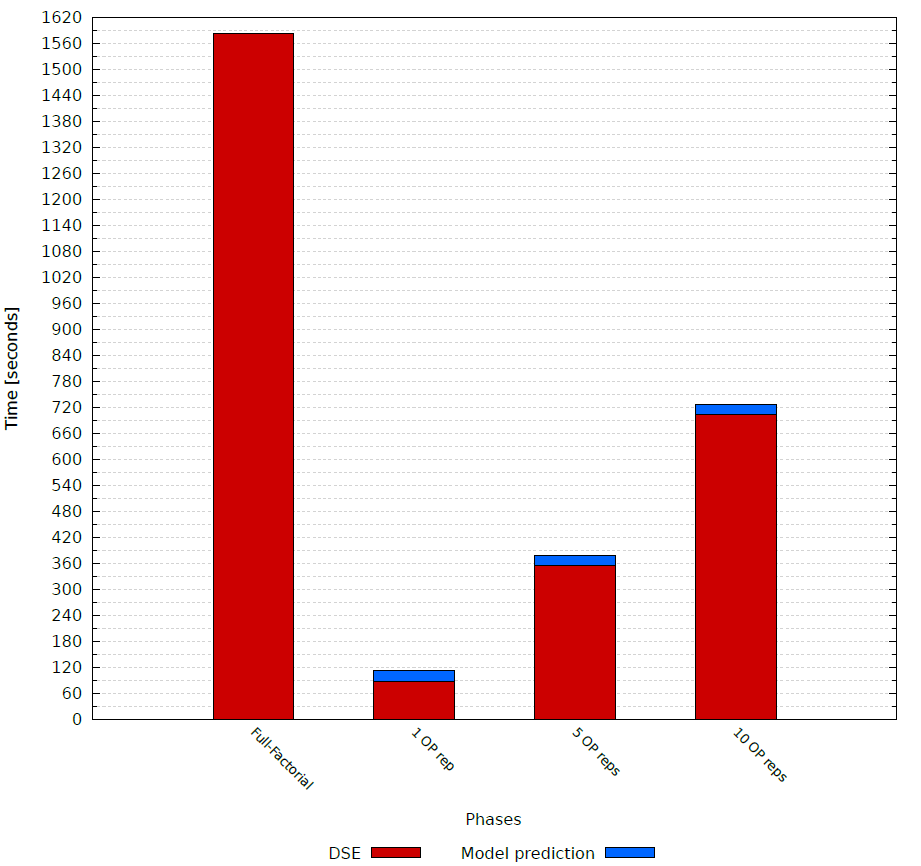
\includegraphics[width = \textwidth]{fullFactorial_tesiCrisPNG}
    \caption{Overall execution time by varying synthetic application version 2 setting}
    \label{fig::full_cris}
    
\end{figure}

Figure \ref{fig::full_cris} shows that an exhaustive execution of analyzed application takes more than 26 minutes to finish. With the introduction of Agora, using Face Centered Central Composite Desing of Experiments with one Center Point and the 2nd version of implemented GLR as RSM, overall time becomes 12 minutes if 10 repetitions for each DoE configuration are collected, about 6 minutes with 5 repetitions and even around 2 minutes with 1 repetition. We specify that, if we want to explore every possible configuration in the exhaustive analysis as much as we do for 5 and 10 OP repetitions of DoE configurations with Agora, of course overall time is 130 minutes and 260 minutes respectively (5 times and 10 times the shown serial execution time), increasing much more the gap between Full-Factorial execution and the ones with the supervise of this work. Finally, we also want to remind, from Figures \ref{fig::synth2spark2::intervals} and \ref{fig::synth2spark2::means}, that Agora, for this application setting, can predict a complete model with a very high quality even collecting just 1 repetition for each DoE configuration, so the final result is very similar to an exhaustive analysis. Therefore, this work can produce high benefits in the prediction of application complete model, starting from a small subset of configurations.


\subsubsection{Application behavior over time}

\begin{figure}[htb]

    \centering
    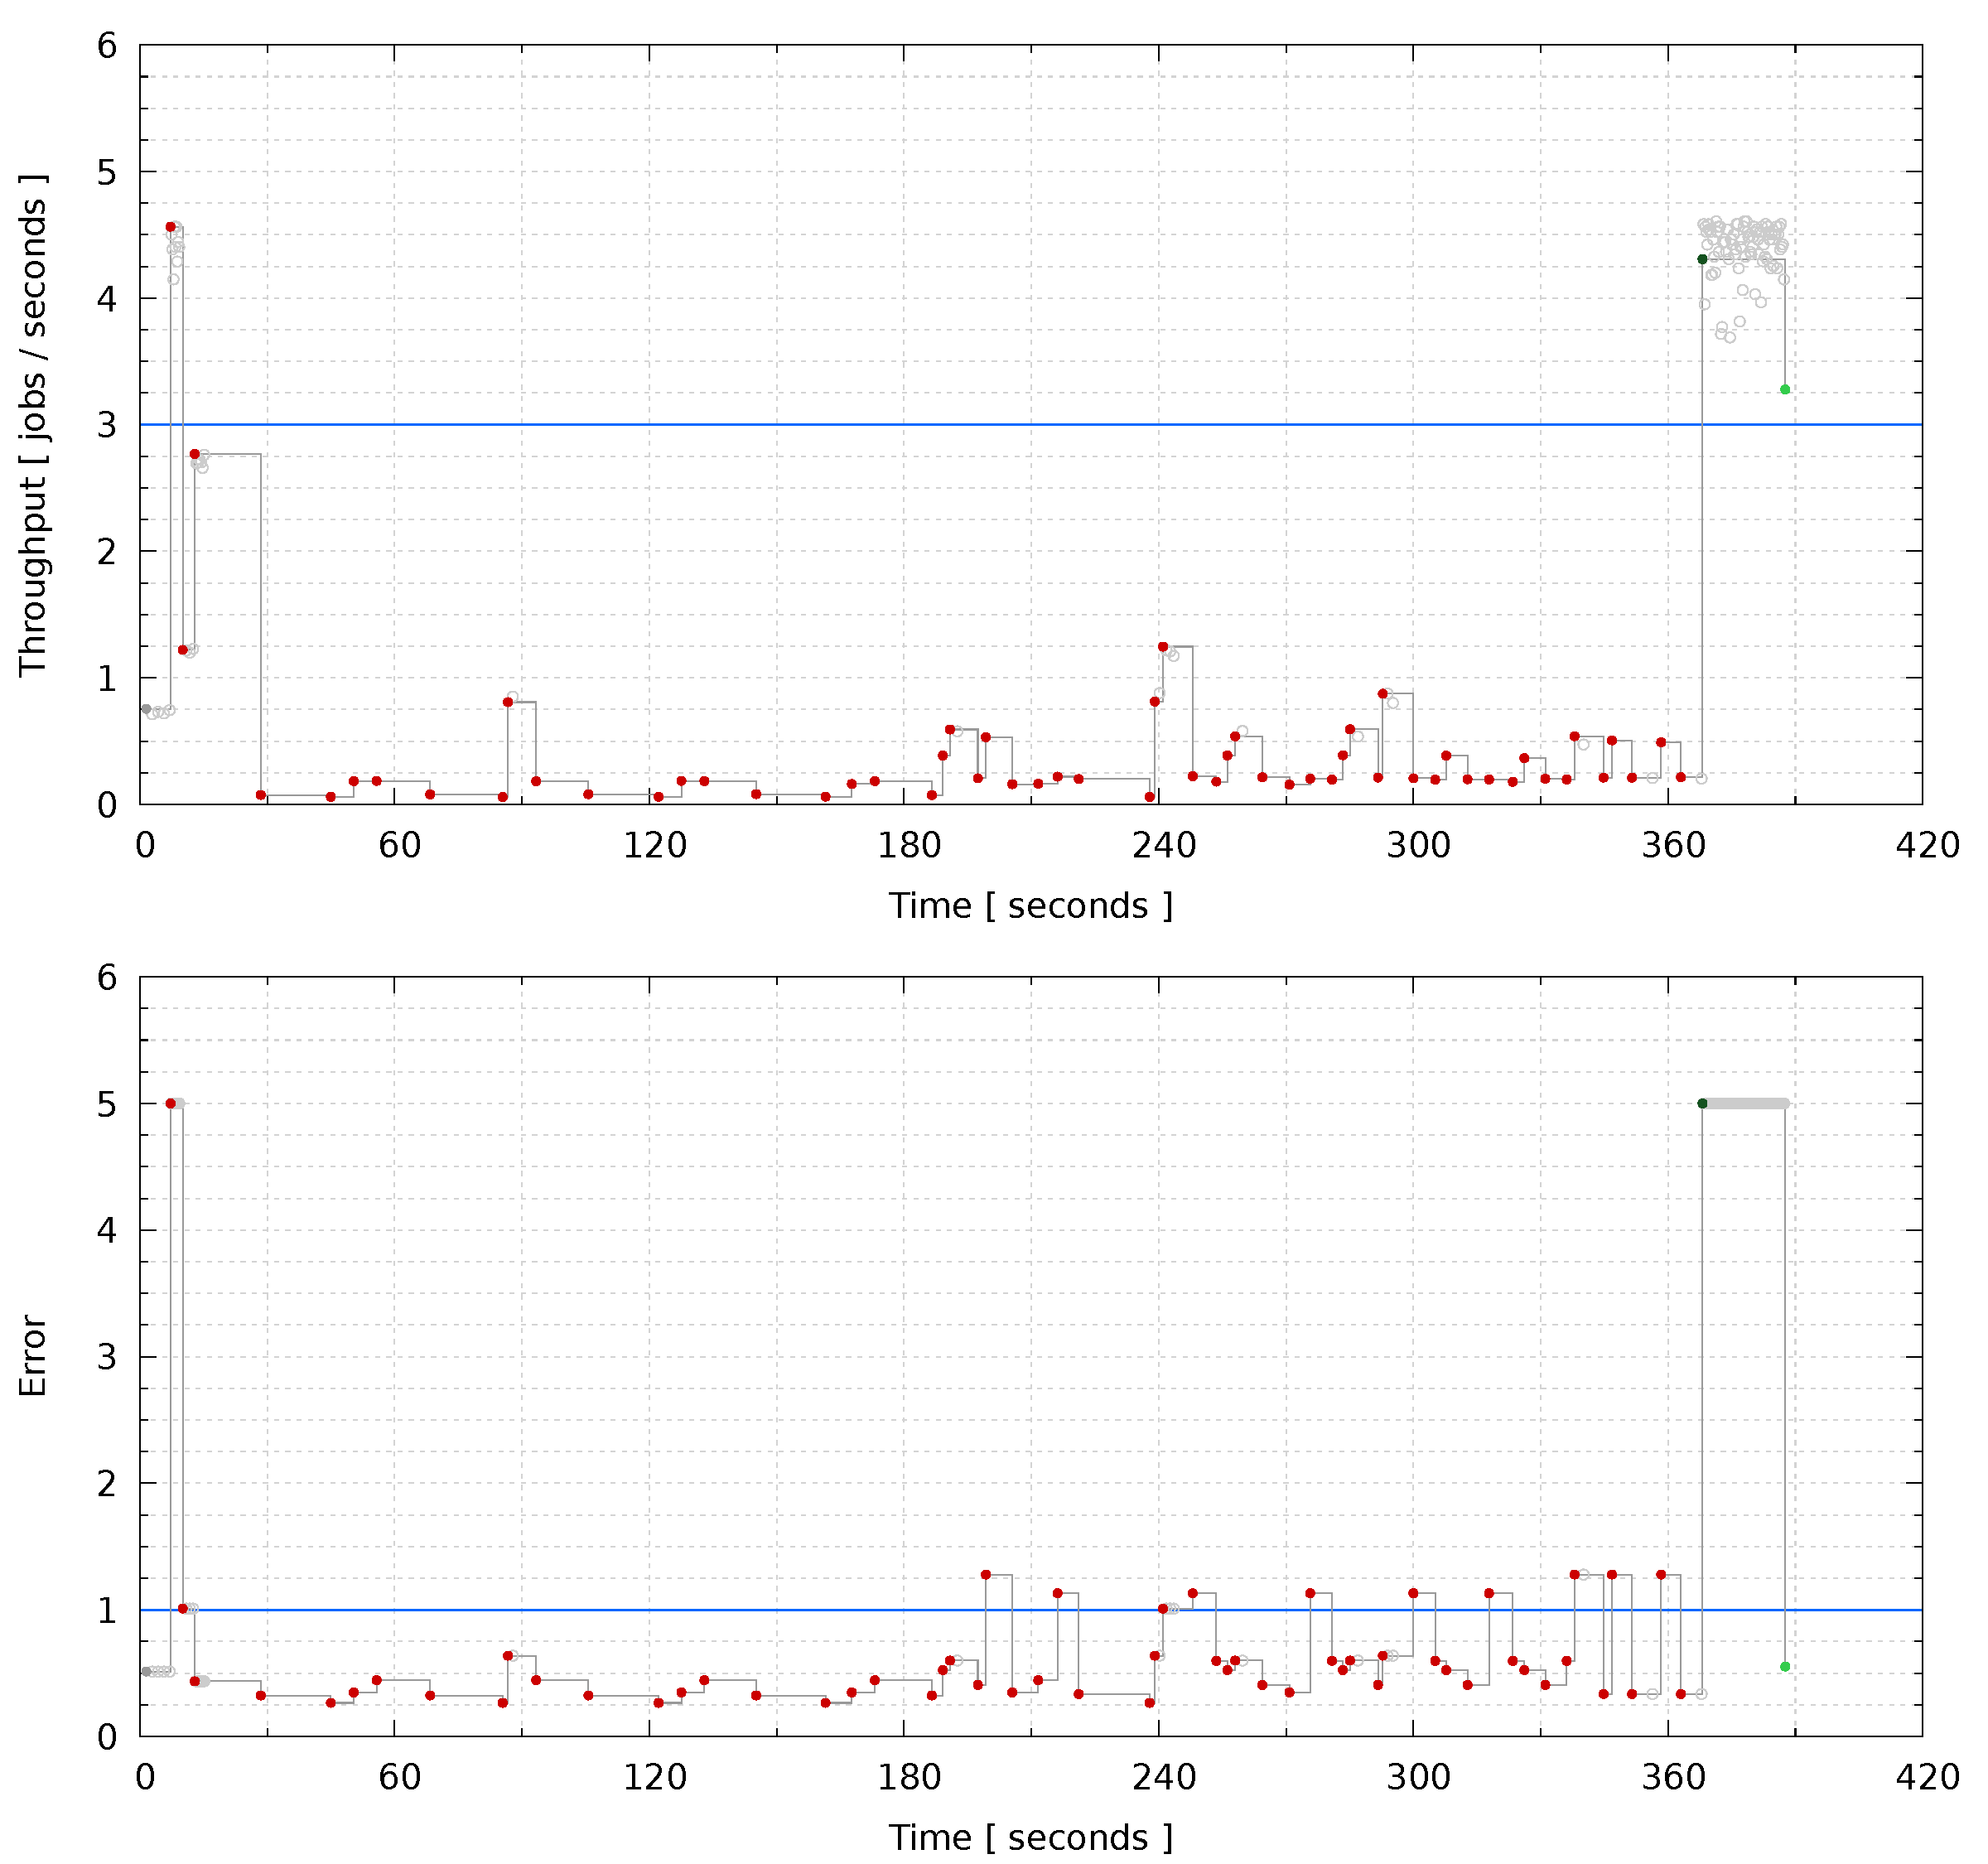
\includegraphics[width = \textwidth]{appBehavior}
    \caption{Metric values of synthetic application version 2 by varying time}
    \label{fig::appBeh}
    
\end{figure}

Figure \ref{fig::appBeh} wants to show application behavior during execution with the supervise of Agora and mARGOt autotuner; on x-axis there is time, while on y-axis there are observed metric of interest values during execution. We have run synthetic application version 2 with $noisePercentage = 15\%$, using Face Centered Central Composite Design of Experiments with one Center Point and the 2nd version of implemented GLR as RSM, collecting 5 repetitions for each Design of Experiments configuration during DSE phase. Objective functions have been set up to $Throughput > 3$ and $Error < 1$.

Every couple of corresponding points in graphs of Figure \ref{fig::appBeh} represents a configuration with which the application has been executed, obtaining certain throughput and error metric values. From a colored couple of points to the following one, the application has maintained parameter values corresponding to the former couple. Grey empty couples of points indicate application execution with parameter values equal to the first previous colored couple. At the beginning, application runs with default configuration, corresponding to an error of around 0.5 and a throughput equal to about 0.75 (black couple of points). Agora starts Design Space Exploration, sending DoE configurations; mARGOt, from time to time, sets application parameters with these values, so observed metric of interest values vary during all this phase (red couples of points). When DSE phase terminates, Agora sends a partial model (see Chapter \ref{DoEModelSend}) and it starts predicting the complete list of Operating Points; mARGOt chooses the best application configuration that fulfills objective functions, represented by dark green couple of points. Throughput is around 4.25, so the first goal is respected, while error is about 5, so the second goal is not achieved (blue lines highlight boundaries of objective functions). When application receives the complete model (around at 6 and a half minutes after starting time), it is set with another configuration (light green couple of points): obtained throughput is approximately 3.25 and error is about 0.5, so all objective functions are fulfilled. Of course, if objective functions don't change, program keeps running with this Operating Point.





\subsection{Swaptions application}

\begin{figure}[htb]

    \centering
    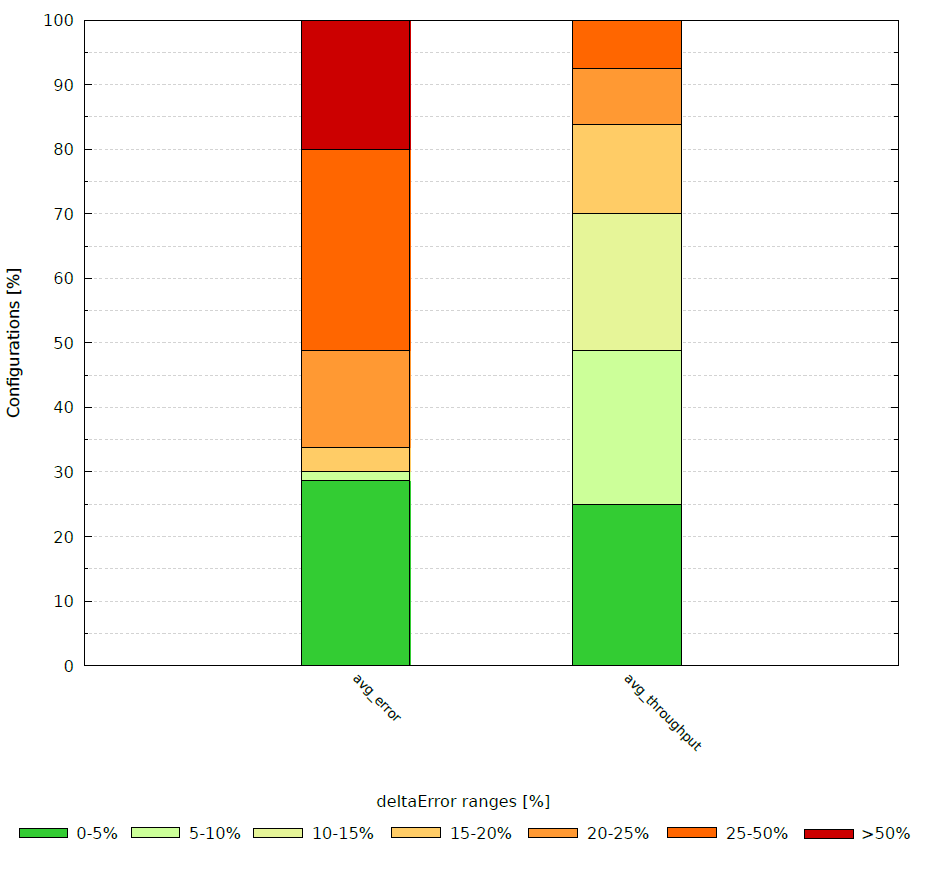
\includegraphics[width = \textwidth]{deltaErrorRangesSwaptions15Spark2PNG}
    \caption{$deltaError$ results for both Swaptions metrics of interest}
    \label{fig::swaptions15spark2::intervals}
    
\end{figure}

\begin{figure}[htb]

    \centering
    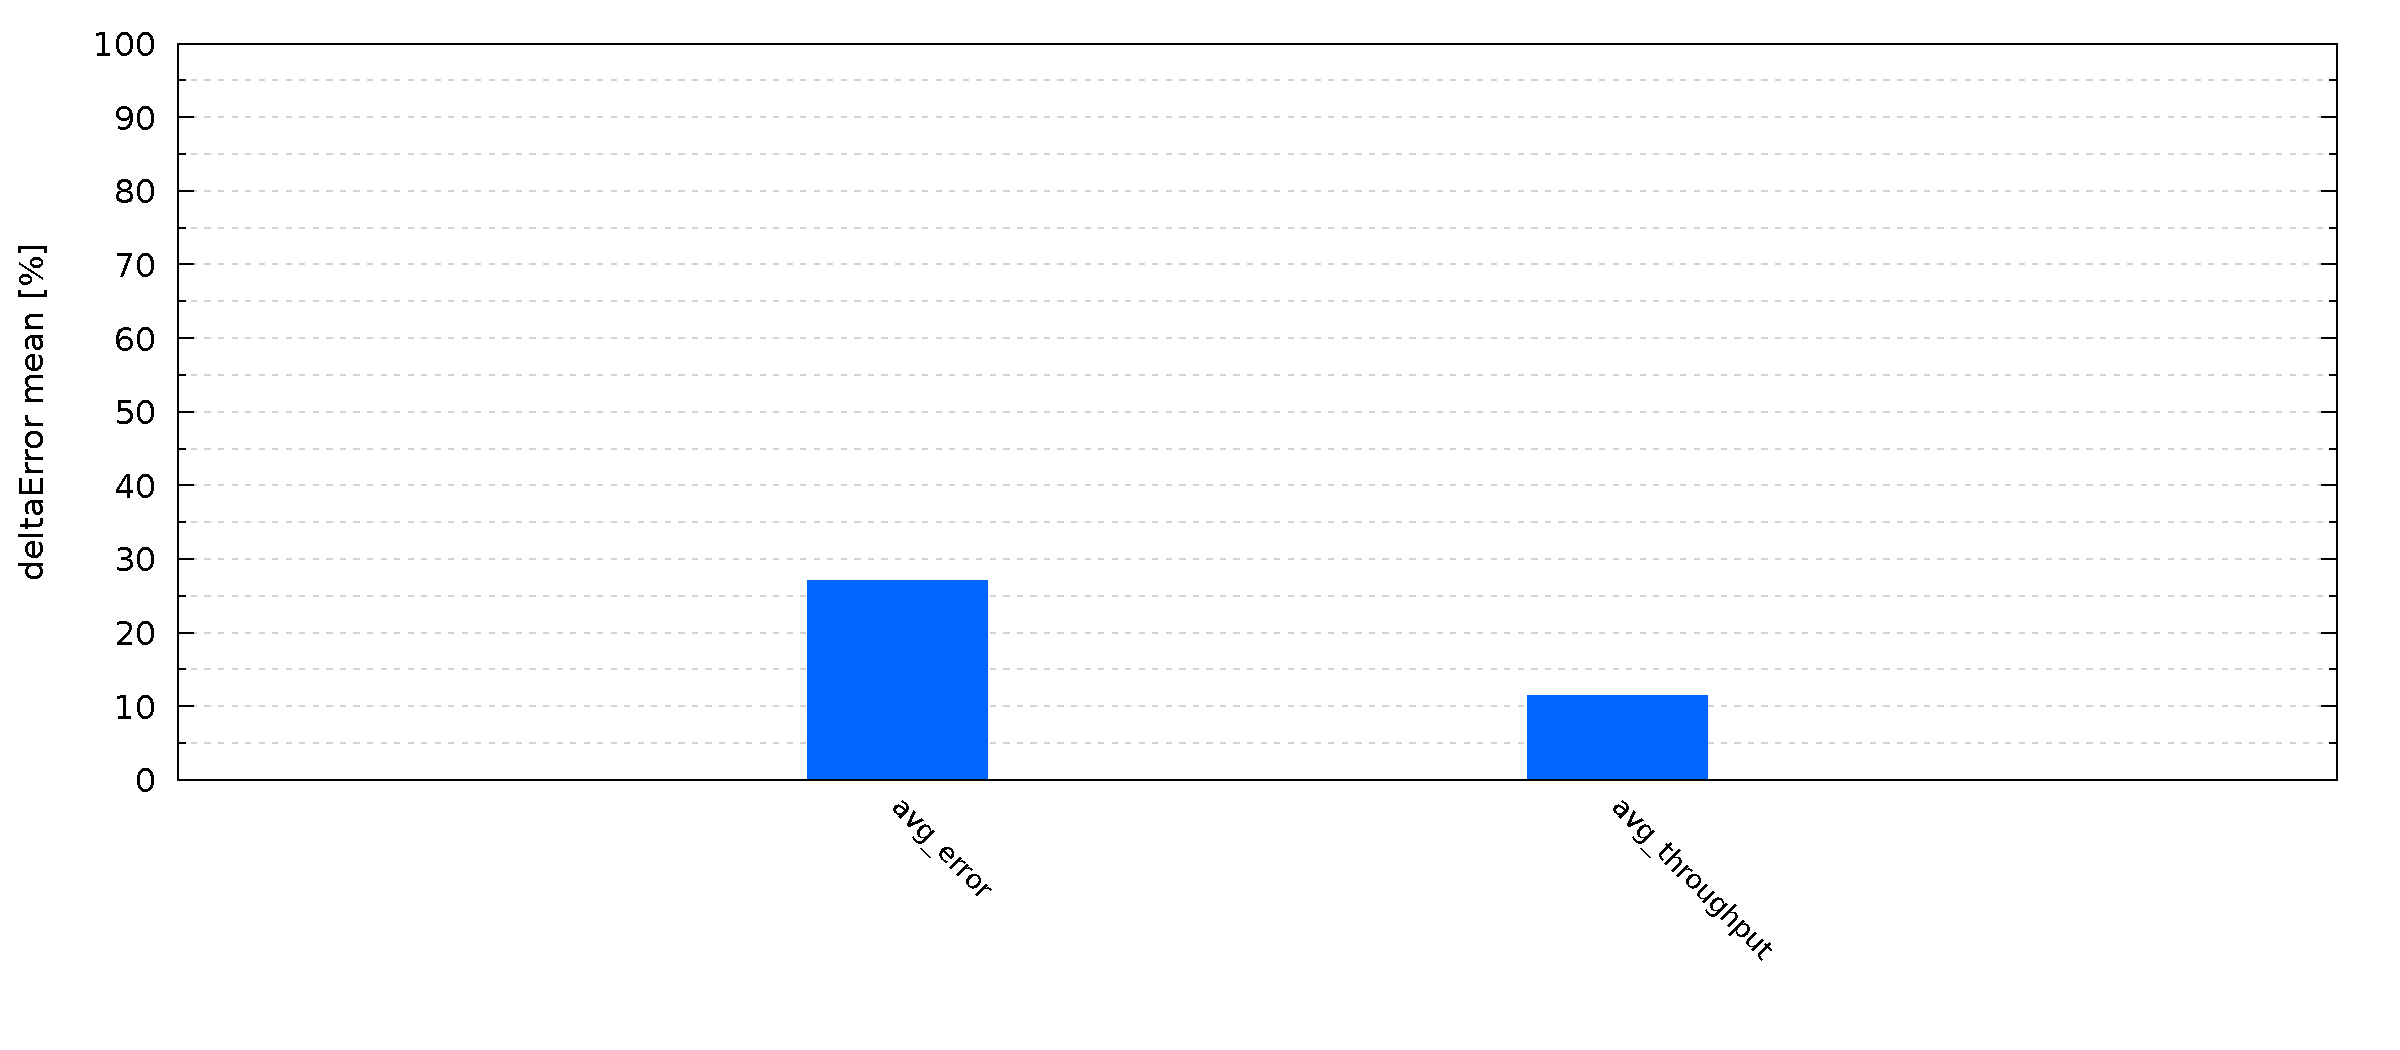
\includegraphics[width = \textwidth]{deltaErrorMeansSwaptions15Spark2}
    \caption{$deltaError$ mean values for both Swaptions metrics of interest}
    \label{fig::swaptions15spark2::means}
    
\end{figure}	

We evaluate Agora on a real scenario. We use Face Centered Central Composite DoE with One Center Point as Design of Experiments and the 2nd version of implemented Generalized Linear Regression as Response Surface Methodology. Due to application computing kernel (Monte Carlo simulations), we have decided to collect, for each DoE configuration, a meaningful number of repetitions, setting this value to 15.


\subsubsection{Model prediction quality}

Figures \ref{fig::swaptions15spark2::intervals} and \ref{fig::swaptions15spark2::means} show results on predicted model using $deltaError$ measure, as done for synthetic application analysis (see \ref{deltaErrorExplanation}), for both $avg\_error$ and $avg\_throughput$ metrics.

We obtain an average $deltaError$ of around $11\%$ for $avg\_throughput$ and about $27\%$ for $avg\_error$, as it is shown in Figure \ref{fig::swaptions15spark2::means}. From Figure \ref{fig::swaptions15spark2::intervals} we can see that $70\%$ of $avg\_throughput$ predictions has a $deltaError$ below $15\%$, while this percentage increases to $30\%$ for $avg\_error$ metric.


\subsubsection{Execution times}

\begin{figure}[htb]

    \centering
    
    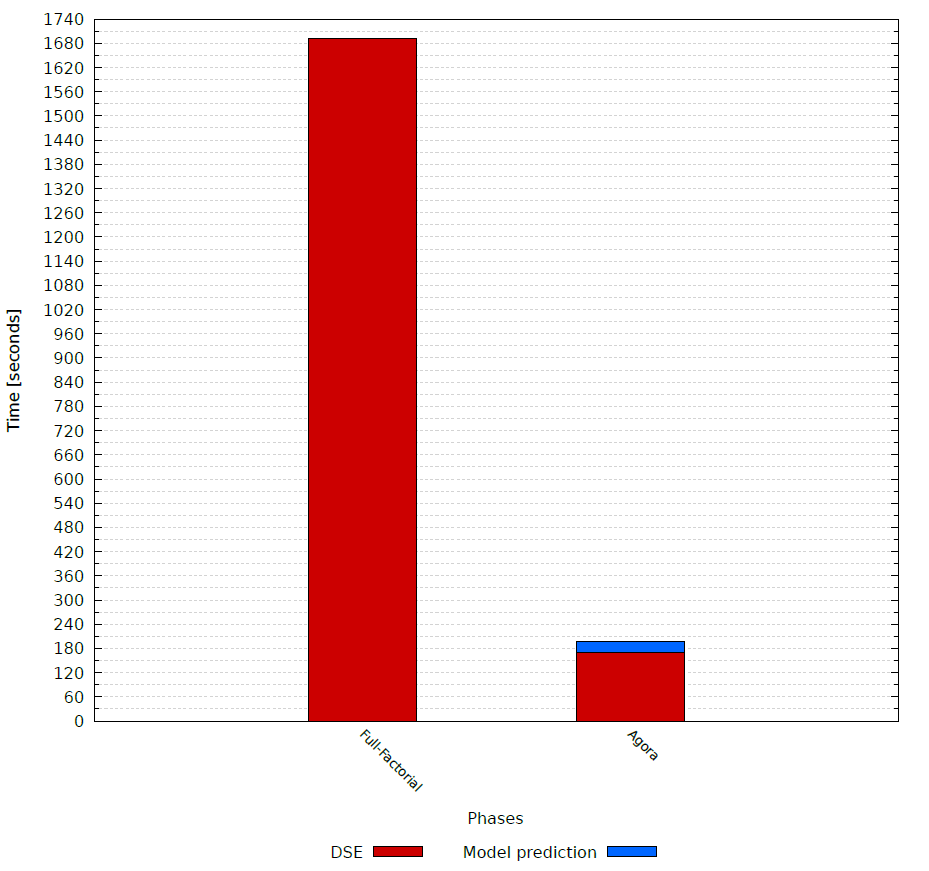
\includegraphics[width = \textwidth]{swaptions_exhaustive_tesiCrisPNG}
    
    \caption{Swaptions execution times}
    
    \label{fig::sw::execT}
    
\end{figure}

Regarding execution times, we compare analyzed run with a Full-Factorial, so exhaustive, execution in which we collect, for each configuration, 15 repetitions for each Operating Point, as shown in Figure \ref{fig::sw::execT}. Exhaustive execution takes around 28 minutes to finish, while the analyzed one less than 3 and a half minutes, so approximately 8 times less. Of course, as explained before, we do not obtain precise predictions for each metric value; nevertheless, Swaptions can be executed with the assistance of Agora plus mARGOt autotuner and, finally, prearranged objective functions are achieved, also because mARGOt is able to collect feedback information that corrects application model.


\subsubsection{Application behavior over time}

\begin{figure}[htb]

    \centering
    
    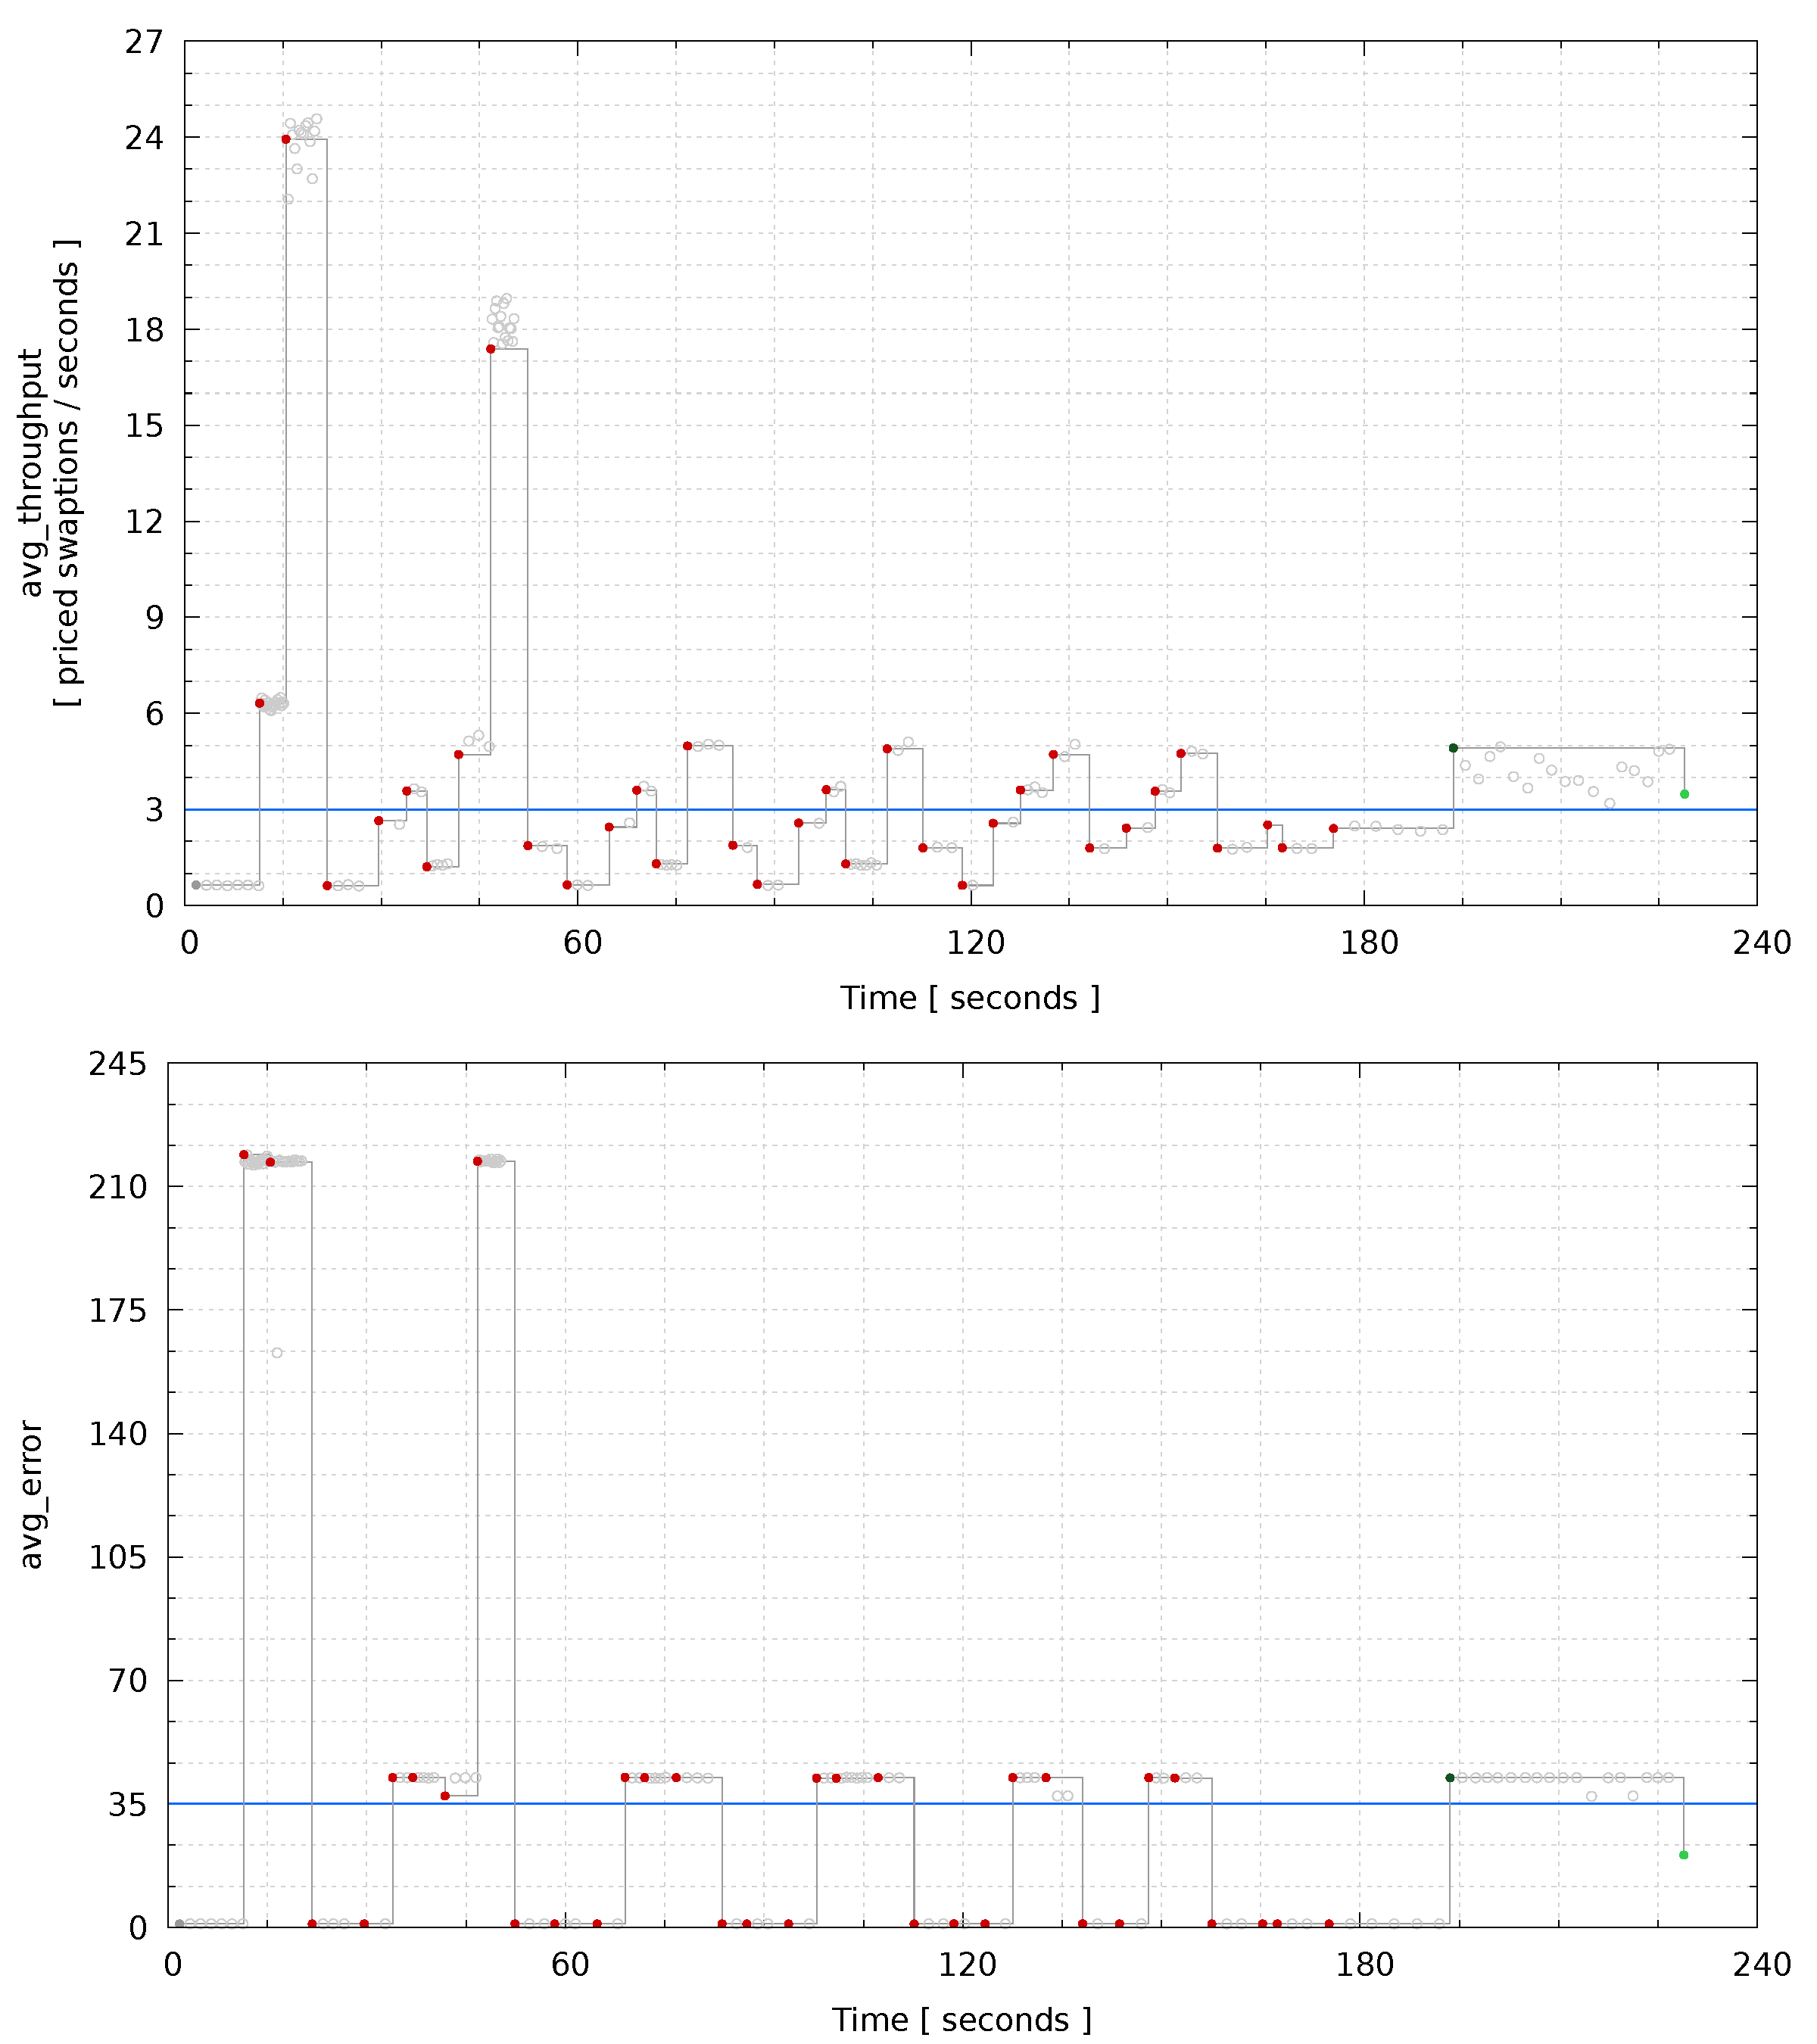
\includegraphics[width = \textwidth]{swaptionsBehavior}
    
    \caption{Swaptions metric values by varying time}
    
    \label{fig::sw::beh}
    
\end{figure}

Figure \ref{fig::sw::beh} shows application behavior during execution. We set, as objective functions, $avg\_\-throughput > 3$ and $avg\_\-error < 35$ (blue lines highlight boundaries of objective functions). During Design Space Exploration phase, application is executed with Design of Experiments configurations in order to collect training data (red couples of points). Around 195 seconds, DSE phase finishes and application receives partial model (see Chapter \ref{DoEModelSend}). mARGOt sets up Swaptions with best possible parameter values with respect to goals and requirements (dark green couple of points): during model prediction phase, $avg\_throughput$ is about 5 (so, great\-er than the minimum required value 3) and $avg\_error$ approximately 42 (higher than 35, so the corresponding objective function is not followed). Agora sends complete model with predicted metric values for each application configuration; mARGOt changes current Operating Point (light green couple of points), obtaining an $avg\_throughput > 3$ and an $avg\_error < 35$, so both objective functions are achieved. 

\chapter{Conclusions and Future Works}\label{end}

\lettrine{W}{}\textit{e} have presented \textit{Agora}, a supporting framework designed to provide predicted complete model of tunable applications, including the whole list of parameter settings and related metric of interest performance. \textit{Agora} faces High Performance Computing application issues related to the problem of exploring design space in an exhaustive way, due to its significant dimension. Main goal is to collect information about a small subset of possible application configurations and, through this data and Machine Learning techniques, to predict general program behavior in all possible paratemer value combinations.

Unique \textit{Agora} feature is the ability to remotely drive Design Space Exploration phase among same executing applications at runtime, distributing all configurations to be explored in an efficient way, therefore every running program contributes to data collection and the entire workflow is considerably sped up. We remark that analysis is not done locally in every node of a possible parallel architecture, but it is accomplished outside, not consuming, in this way, node computational capacity, except for communications among \textit{Agora} modules, fulfilled by the lightweight MQTT messaging protocol.

In this thesis we show \textit{Agora} benefits, in terms of model prediction quality, execution times and ability to drive application executions in the reported experimental result, through multiple versions of a synthetic program with analytical metrics and a real scenario, using \textit{Swaptions} application from the PARSEC benchmark suite (\cite{bienia2008parsec}). We demonstrate that in several scenarios, even introducing strong noises, we are able to achieve very high model prediction quality and, having the possibility to use multiple executing nodes to explore application Design Space, we demonstrate how overall time strongly decreases with respect to an individual analysis with a single application: at the best of our knowledge, this is the first attempt to share Design Space Exploration as supervised by \textit{Agora}.

There are, certainly, several elements of our work that can be envisioned as future steps:

\begin{enumerate}

	\item in addition to implemented Machine Learning strategies (two versions of Generalized Linear Regression, see Chapter \ref{regrTransforms}), there can be added other techniques, in order to expand and to improve \textit{Agora} versatility. Moreover, instead of entrusting to user the selection of Machine Learning strategy, the system could be able to analyze current problem and to choose itself best technique among the available ones in a proper way;

	\item after application model prediction, \textit{Agora} could continue to collect feedback information about program execution, in order to eventually update model and send again revised complete list of application configurations with related predicted performance in terms of metric of interest values;

	\item there could be added the possibility to specify a limit duration of Design Space Exploration phase: when time is up, \textit{AgoraRemoteAppHandler} module predicts application complete model with all information collected up to that moment;

	\item instead of specifying a priori application lapse for request (see Chapter \ref{clientReq}), \textit{AgoraLocalAppHandler} module could dynamically a\-dapt request frequency, according to previous execution times.

\end{enumerate}

We hope \textit{Agora} can contribute to the research on Design Space Exploration and Dynamic Autotuning of High Performance Computing applications in parallel architectures.


\cleardoublepage
\newpage

%%%%%%%%%%%%%%%%%%%%%%%%%%%%%%%%%%%%%%
% Acknowledgement
%%%%%%%%%%%%%%%%%%%%%%%%%%%%%%%%%%%%%%
\chapter*{Ringraziamenti}

\begin{otherlanguage}{italian}





Sono giunto a conclusione di un lungo e faticoso percorso di studi. Il mio pensiero non può non andare a tutte quelle persone che, chi da sempre e chi da molto, fanno parte della mia vita e che, in quest'ultima prova, mi sono state vicine. Voglio ringraziare:


\par\bigskip


la relatrice Prof.ssa Cristina Silvano e i correlatori Davide Gadioli e il Prof. Gianluca Palermo, che mi hanno guidato e assistito durante gli ultimi nove mesi: senza di loro questa tesi non sarebbe stata possibile;


\par\bigskip


i miei amici, di vecchia e più recente data, di Sulmona (e dintorni) e di "cittadinanza onoraria" milanese, presenti nella maggior parte dei miei felici ricordi, senza i quali la vita sarebbe terribilmente più noiosa;


\par\bigskip


mia sorella Giulia, punto fermo e certezza, senza la quale sarei indubbiamente più solo;


\par\bigskip


mia madre Luciana e mio padre Romano, senza i quali io non sarei nulla;


\par\bigskip


Claudia, senza la quale nulla sarebbe.


\par\bigskip


\begin{flushright}

	Grazie di cuore a tutti voi,\\\textit{Cristiano}

\end{flushright}





\end{otherlanguage}


\cleardoublepage
\newpage

%\cleardoublepage
%\listoffigures
%\listoftables

\cleardoublepage
\phantomsection
\addcontentsline{toc}{chapter}{\bibname}
\small
\bibliographystyle{plain}
\bibliography{thesis}

\end{document}
